\documentclass{article}

% Formatting
\DeclareUnicodeCharacter{2060}{\nolinebreak} % Prevent unicode (U+2060) error on local complile
\frenchspacing % No double spacing between sentences
\hbadness=1000000 % Turn off \hbox badness warnings
\linespread{1.2} % Set linespace


% Packages
\usepackage[a4paper, left=1.5cm, right=1.5cm, top=1.5cm, bottom=1.5cm]{geometry}
\usepackage{authblk} % For author formatting
\usepackage{caption} % For figure and table captions
\usepackage{cclicenses} % For creative commons license
\usepackage{float} % To force figure location after text
\usepackage{graphicx} % Adds more functionality to graphics for inclusion of figures
\usepackage{lscape} % For landscape pages
\usepackage{lineno} % Allows use of \linenumbers to add line numbers 
\usepackage{lmodern} % A scalable font - avoids erros due to non-sclabale fonts
\usepackage{longtable,booktabs}  % For tables
\usepackage{markdown} % Allow use of markdown syntax
\usepackage{microtype} % 'Improved' typesetting
\usepackage[nottoc,numbib]{tocbibind} % Add references to table of contents
\usepackage{parskip} % Adds white space between paragraphs
\usepackage{pdflscape} % To create landscape pages that show as landscape in PDF viewer
\usepackage{placeins} % to use \FloatBarrier where want a hard break between content (to force and order of text and figures
\usepackage{ragged2e} % Better right ragged edges (allows hyphenation)
\usepackage{subcaption} % Allows use of subfigures
\usepackage[super]{natbib} % Citations using superscript
\usepackage{titlesec} % For title spacing
\usepackage[toc,page]{appendix}
\usepackage{url} % Tidy web links
\usepackage[utf8]{inputenc}
\usepackage{verbatim}
\usepackage{xcolor} % For coloured text
\usepackage{xurl} % For url but with more flexible linebreaking


% Choose your own colour
\usepackage{color}
\newcommand{\mjanote}[2][\textcolor{red}{\dagger}]{\textcolor{red}{$#1$}\marginpar{\color{red}\raggedright\tiny$#1$ #2}}
\newcommand{\mjaFIXME}[1]{\textcolor{red}{[\textbf{FIXME} \textsl{#1}]}}
\newcommand{\kpnote}[2][\textcolor{magenta}{\dagger}]{\textcolor{magenta}{$#1$}\marginpar{\color{magenta}\raggedright\tiny$#1$ #2}}
\newcommand{\kpFIXME}[1]{\textcolor{magenta}{[\textbf{FIXME} \textsl{#1}]}}


% Info on wordcounts:
% https://www.overleaf.com/learn/how-to/Is_there_a_way_to_run_a_word_count_that_doesn%27t_include_LaTeX_commands%3F

% To include refs in word count:
%TC:incbib

\newcommand{\detailtexcount}[1]{%
  \immediate\write18{texcount -merge -sum -q #1.tex output.bbl > #1.wcdetail }%
  \verbatiminput{#1.wcdetail}%
}

% Count tables in wordcount

%TC:group table 0 1
%TC:group tabular 1 1

\begin{document}

% Ignore title and abstract in word count
%TC:ignore
\title{Stroke Audit Machine Learning (SAMueL-2)}
\date{August 2024}


\renewcommand{\thefootnote}{\fnsymbol{footnote}}

\author[*1,2]{Michael Allen}
\author[1,2]{Kerry Pearn}
\author[1]{Rachel Jarvie}
\author[1]{Anna Laws}
\author[1]{Julia Frost}
\author[1]{Leon Farmer}
\author[3]{Peter McMeekin}
\author[4]{Catherine Pope}
\author[1]{Iain Lang}
\author[1]{Keira Pratt-Boyden}
\author[1]{Richard Everson}
\author[1,5]{Martin James}

% Check affiliations - update RDE Name
\affil[1]{\footnotesize University of Exeter Medical School}
\affil[2]{\footnotesize NIHR South West Peninsula Applied Research Collaboration (ARC)}
\affil[3]{\footnotesize Northumbria University}
\affil[4]{\footnotesize University of Oxford}
\affil[5]{\footnotesize Royal Devon University Healthcare NHS Foundation Trust}
\affil[*]{\footnotesize Corresponding author: m.allen@exeter.ac.uk}

\maketitle
%TC:endignore

\tableofcontents

\newpage
%TC:ignore
\section*{Abstract} %* makes it not numbered
\addcontentsline{toc}{section}{Abstract} %Add non-numbered section to table of contents

\textbf{Background}

Use of thrombolysis to treat emergency stroke patients varies considerably between hospitals. Previous work has shown that the majority of this variation comes from between-hospital decision-making on which patients should receive thrombolysis.

\textbf{Key objectives}

\begin{itemize}

    \item Understand how patient characteristics affect decisions to use, or not use, thrombolysis at each hospital.

    \item Predict expected outcomes for patients, with and without thrombolysis, and investigate whether hospitals with higher use of thrombolysis are likely to be generating more patient benefit. 
    
    \item Predict how thrombolysis affects Quality of Life Years (QALYs).

    \item Model patient flow (including ambulance response times) and predict how process changes would affect thrombolysis use and benefit.

    \item Generation of a web-based dashboard to allow clinicians to interrogate modelling.

    \item Co-production of project outputs with clinicians to promote acceptance and use for local quality improvement, and investigate how well organisation factors predict thrombolysis use, to identify whether aspects of the organisation impacts the decision to treat.

\end{itemize}

\textbf{Methods}

\begin{itemize}

    \item Co-production and qualitative research used observation, semi-structured interviews, and review of NHS documents.

    \item Patient flow through the emergency stroke pathway was modelled with Monte-Carlo simulation, and a mathematical model of outcome based on  clinical trial results.

    \item  Thrombolysis decisions and outcomes (with and without thrombolysis) were predicted using XGBoost machine learning, with Shapley values  generated to show the contribution of individual features to the prediction.
    
\end{itemize}

\textbf{Results}

\begin{itemize}

    \item Qualitative research showed that participants were hopeful the SAMueL-technology could address variance in thrombolysis practice. It was seen as particularly suitable for less experienced clinicians and offered value for training, reviewing clinical cases, and quality improvement. It is important to reassure intended adopters about the integrity of modelling based on this data. Evidence indicated that emergency department physicians may have less confidence in the evidence base for thrombolysis.
    
    \item Machine learning demonstrated that thrombolysis was having at least the expected clinical benefit as predicted by the clinical trials. On average, it was predicted that thrombolysis adds 0.26 QALY for each person treated. Stroke teams with higher thrombolysis use are predicted to be generating better patient outcomes.
    
    \item Factors that most affect thrombolysis use in ischaemic stroke are arrival-to-scan time, stroke severity, prior disability, and hospital attended. After adjusting for other patients features, the odds of receiving thrombolysis varied 13-fold between hospitals.
    
    \item Factors  that most affect outcome after stroke are pre-stroke disability, stroke severity, age and use/time of thrombolysis.
    
    \item By combining changes to processes and decision-making there is potential to increase thrombolysis use from 13\% to 20\% in patients arriving by ambulance. Improving pathway speed has a greater effect on outcomes than on thrombolysis use. A web tool allows interrogation at the level of stroke team.
\end{itemize}


\textbf{Conclusions}

Thrombolysis was, using observational data, was found to have at least as much benefit as predicted by the clinical trial meta-analysis. Variation in decision-making concerning thrombolysis is leading to significant between-hospital variation in thrombolysis use, and is leading to variation in outcomes. Stroke teams with higher thrombolysis use are predicted to be generating better patient outcomes. 

\section*{Plain Language Summary}
\addcontentsline{toc}{section}{Plain Language Summary}

\textbf{What is the problem?} Use of clot-busting treatment in stroke varies a great deal between hospitals.

\textbf{What did we know?} We knew that the largest cause of this variation was differences between hospitals in which patients they choose to give  clot-busting treatment to. Some doctors are worried that the risk from this treatment can often outweigh the benefits, and worry that use of this treatment in the real world won’t have the same benefit that the clinical trials predicted it would have.

\textbf{What did we not know?} We did not know how the variation in use of clot-busting treatment was affecting outcomes. We didn’t know what it was about the patients that doctors considered when making decisions, and we didn’t know what most affected patient outcome. We didn’t know what doctors would think of using ‘Artificial Intelligence’ to help understand answers to these questions.

\textbf{What did we do?} We used ‘Artificial Intelligence’ to learn which patients different hospitals would give lot-busting treatment to, and to learn which patients would likely have a better outcome if this treatment was used.

\textbf{What did we find out?} We found out that clot-busting treatment was at least as effective in real use as the clinical trials predicted, and hospitals choosing to use it more are very likely saving more lives and reducing disability from stroke. We now understand what doctors look at when deciding to use it or not, and what affects patient outcomes. We  found out speeding up giving this treatment would improve the number of people who could receive it, and would mean everyone receiving it would benefit more from it. We found that doctors were interested in our work, but they need to be convinced our ‘Artificial Intelligence’ is right, but we are hopeful that our results will give doctors more confidence to use this treatment more often, and to always give it as fast as possible.
%TC:endignore
\section{Introduction}

% Include
% 1) What is the problem?
% 2) What do we know about low and varying use of thrombolysis
% 3) What do we not know
% 4) How are we addressing what we don't know

% 1) What is the problem?

Stroke remains one of the top three global causes of death and disability \cite{feigin_global_2021}. Despite reductions in age-standardised rates of stroke, ageing populations are driving an increase in the absolute number of strokes \cite{feigin_global_2021}. Across Europe, in 2017, stroke was found to cost healthcare systems \texteuro 27 billion, or 1.7\% of health expenditure \cite{luengo-fernandez_economic_2020}. Thrombolysis with recombinant tissue plasminogen activator, can significantly reduce disability after ischaemic stroke, so long as it is given in the first few hours after stroke onset \cite{emberson_effect_2014}. Despite thrombolysis being of proven benefit in ischaemic stroke, use of thrombolysis varies significantly both between and within European countries \cite{aguiar_de_sousa_access_2019}. In England and Wales the national stroke audit reported that in 2021/22, 20 years on from the original European Medicines Agency licensing of alteplase for acute ischaemic stroke, thrombolysis rates for emergency stroke admissions varied from just 1\% to 28\% between hospitals \cite{sentinel_national_stroke_audit_programme_ssnap_2022}, with a median rate of 10.4\% and an inter-quartile range of 8\%-13\%, against a 2019 NHS England long term plan that 20\% of patients of emergency stroke admissions should be receiving thrombolysis \cite{nhs_long_term_plan_2019}.

The NHS plan for improving stroke care also sets a target that patients should receive thrombolysis within 60 minutes of arrival, but ideally within 20 minutes (12). Whilst this speed of thrombolysis, called door-to-needle time, provides an ambitious target, it has been shown to be achievable as Helsinki University Central Hospital has reported a median door-to-needle time of 20 minutes, with 94\% of patients treated within 60 minutes \cite{meretoja_reducing_2012}.

% 2) What do we know about low and varying use of thrombolysis

Studies have shown that reasons for low and varying thrombolysis rates are multi-factorial. Reasons include late presentation \cite{aguiar_de_sousa_access_2019}, lack of expertise \cite{aguiar_de_sousa_access_2019} or lack of clear protocols or training \cite{carter-jones_stroke_2011}, delayed access to specialists \cite{kamal_delays_2017}, and poor triage by ambulance or emergency department staff \cite{carter-jones_stroke_2011}. For many factors, the establishment of primary stroke centres has been suggested to improve the emergency care of patients with stroke and reduce barriers to thrombolysis \cite{carter-jones_stroke_2011}, with a centralised model of primary stroke centres leading to increased likelihood of thrombolysis \cite{lahr_proportion_2012, morris_impact_2014, hunter_impact_2013}. 

In addition to organisational factors, clinicians can have varying attitudes to which patients are suitable candidates for thrombolysis. In a discrete choice experiment \cite{de_brun_factors_2018}, 138 clinicians considered hypothetical patient vignettes, and responded as to whether they would give the patients thrombolysis. The authors concluded that there was considerable heterogeneity among respondents in their thrombolysis decision-making. Areas of difference were around whether to give thrombolysis to mild strokes, to older patients beyond 3 hours from stroke onset, and when there was pre-existing disability.

Based on national audit data from three years of emergency stroke admissions, we have previously built models of the emergency stroke pathway using clinical pathway simulation to examine the potential scale of the effect of changing two aspects of the stroke pathway performance (1. the in-hospital process speeds, and 2. the proportion of patients with a determined stroke onset time), and using machine learning to examine the effect of replicating clinical decision-making around thrombolysis from higher thrombolysing hospitals to lower thrombolysing hospitals \cite{allen_using_2022, allen_use_2022}. The machine learning model learned whether any particular patient would receive thrombolysis in any particular emergency stroke centre. Using these models we found that it would be credible to target an increase in average thrombolysis in England and Wales, from 11\% to 18\%, but that each hospital should have its own target, reflecting differences in local populations. We found that the largest increase in thrombolysis use would come from replicating thrombolysis decision-making practice from higher to lower thrombolysing hospitals. Two other important factors influencing thrombolysis rates were determination of stroke onset time in some hospitals, and improving the speed of the in-hospital thrombolysis pathway.

% 3) What do we not know

In our previous work we established that we could predict the use of thrombolysis in patients arriving within 4 hours of known stroke onset with 84.3\% accuracy \cite{allen_use_2022}. We could then ask the question "What if this patient attended another hospital - would they likely be given thrombolysis?" As this was a \emph{`black-box'} decision-forest model we could not effectively explain the relationship between patient level data (`features') and their chance of receiving thrombolysis, or identify and explain the features which different hospitals would differ on. In that work we were also only predicting thrombolysis choice; we were not examining outcomes after stroke with and without thrombolysis, which left open the question of whether stroke teams with higher thrombolysis use were likely to be achieving better outcomes. Incorporating explainability of predictions, and predicting outcomes were therefore key objectives for the current study.

The specific objectives for the current study were:

\begin{enumerate}

    \item \textbf{Prediction of outcomes} (including benefit and risk of thrombolysis) at an individual patient level.

    \item \textbf{Inclusion of a health economics model}, to convert outcomes to quality-adjusted life years (QALYs).

    \item \textbf{Improve model transparency and explainability} by 1) model simplification through feature selection, and to 2) the addition of Shapley values to show the contribution of individual features to the prediction \cite{aas_explaining_2020}.

    \item \textbf{Perform patient clustering or sub-setting of patients} to illustrate similarity/differences in thrombolysis decision-making between hospitals.

    \item \textbf{Investigate how well organisation factors (from the SSNAP organisational audit) predict thrombolysis use}, to identify whether aspects of the organisation impacts the decision to treat.

    \item Include ambulance response times in patient flow modelling, and test how improvement of ambulance response time would affect thrombolysis use and benefit.

    \item \textbf{Generation of a web-based dashboard} to allow clinicians to interrogate modelling.

    \item \textbf{Generation of synthetic data and artificial patient vignettes (\textit{virtual patients}, or \textit{prototype patients})} for enhanced sharing of the modelling (sharing working code with data).

    \item \textbf{Co-production of project outputs with clinicians} to promote acceptance and use for local quality improvement.
    
\end{enumerate}
\section{Emergency stroke pathway under study}


\subsection{Data}

\subsection{Data for modelling}

Data was extracted from the Sentinel Stroke National Audit Programme (SSNAP), the national stroke registry for England, Wales and Northern Ireland, for all patients with an out-of-hospital stroke onset for the full calendar years of 2016-2021. The registry contains  patients admitted to all acutely-admitting hospitals, with a case ascertainment of over 90\% when compared to administrative data (Hospital Episode Statistics). The total number of patients was 360,381, of whom 38.5\% arrived within 4 hours of known stroke onset. Of those arriving within 4 hours of known stroke onset 90.4\% arrived by ambulance (71.6\% of those not arriving within 4 hours of known stroke onset arrived by ambulance).

The following data fields from SSNAP were used in the modelling:

\begin{itemize}

    \item \textit{Stroke team}: Stroke team attended (hospital identifier).

    \item \textit{Age}: As midpoint of 5 year age bands.

    \item \textit{Sex}: Sex of patient (male/female).

    \item \textit{Diagnosis of atrial fibrillation}: Did the patient have a diagnosis of atrial fibrillation, either made prior to admission, or during admission?

    \item \textit{Use of anticoagulants}: Use of prior anticoagulant for atrial fibrillation.

    \item \textit{Onset known}: Whether onset was known, and if known whether it was considered to be known precisely or was a best estimate.

    \item \textit{Onset during sleep}: Did stroke occur in sleep? (1 = Yes, 0 = No).

    \item \textit{Onset-to-arrival time}: Time from onset of stroke to arrival at hospital (minutes), when known.

    \item \textit{Prior disability level}: Estimated mRS score prior to stroke.

    \item \textit{Stroke type}: Infarction/haemorrhage.

    \item \textit{Stroke severity}: National Institutes of Health Stroke Scale (NIHSS) score on arrival.

    \item \textit{Arrival-to-scan time}: Time from arrival at hospital to scan (minutes), when known.

    \item \textit{Scan-to-thrombolysis time}: Time from arrival at hospital to scan to treatment with thrombolysis (minutes), when given.

    \item \textit{Disability on discharge}: mRS (0-6) on discharge, includes death (mRS 6) during admission.
    
\end{itemize}

Appendix section {sec:stats} provides descriptive statistics for patients across stroke teams.

See sections \ref{sec:paper_2} to \ref{sec:paper_5} for further details on data used for each component of the modelling work.



\subsubsection{Ethics}

For modelling, as we were using anonymised secondary data, collected for national audit, individual consent is not required. SSNAP has approval under section 251 of the NHS Health and Social Care Act (2006) to collect patient level data on the first six months of patient care (ECC 6- 02(FT3)/2012), without requiring individual patient consent. Access to SSNAP data is managed by the UK Healthcare Quality Improvement Partnership (HQIP), with this project being approved by HQIP (HQIP303). More information on the use of patient data by SSNAP can be found at \url{https://www.strokeaudit.org/ SupportFiles/Documents/Patient-area-documents/Fair-processingstatement-for-patients-v7-0.aspx}

As we are using anonymised secondary data, collected for national audit, used for service evaluation and improvement, no ethical approval is required (confirmed using the NHS Health Research Authority decision aid: https://www.hra-decisiontools.org.uk/ethics/).

\subsection{Data for qualitative research}

Qualitative research used a combination of observations, interviews and documentary analysis. See section \ref{sec:paper_1} for further details.

\subsubsection{Ethics}

NHS Health Research Authority (HRA) \& Health and Care Research Wales (HCRW) approval was provided by the Essex Research Ethics Committee in August 2023 (IRAS 322303; REC reference 23/EE/0124).
\section{Overview of project papers}
\label{sec:papers}

\subsection{Paper 1: Stroke physicians' and staff perspectives on machine learning to optimise thrombolysis decision making in stroke: a qualitative study. \cite{jarvie_stroke_2024}}

\textbf{Study type and population}

Qualitative study: 184 hours of focussed observation in three NHS Trusts in England. Observation of Integrated Stroke Delivery Networks (ISDNs) and other organisations with a strategic overview of stroke services. 20 participants from the three observation sites and five key informants from other sites took part in semi-structured interviews.

\textbf{Key findings}

\begin{itemize}
    \item Participants were hopeful the SAMueL-2 technology could address variance in thrombolysis practice. It was seen as particularly suitable for junior clinicians, non-stroke specialists and at district general hospitals and offered value for training, reviewing clinical cases, and quality improvement.

    \item Given reservations expressed about the underpinning SSNAP data, it is important to reassure intended adopters about the integrity of modelling based on this data.

    \item Evidence indicated that emergency department physicians may have less confidence in the evidence base for thrombolysis.

    \item Perceived lack of funding and stroke workforce shortages may impede quality improvement and adoption of new technologies such as SAMueL-2

\end{itemize}

%%%%%%%%%%%%%%%%%%%%%%%%%%%%%%%%%%%%%%%%%%%%%%%%%%%

\subsection{Paper 2: What would other emergency stroke teams do? Using explainable machine learning to understand variation in thrombolysis practice.\cite{pearn_what_2023}}

\textbf{Study type and population}

Explainable machine learning model to study decision-to-treat with thrombolysis across 132 stroke teams. The model was based on 3 years of all emergency stroke arrivals to hospitals in England and Wales, arriving within 4 hours of stroke onset (88,928 patients).

\textbf{Key findings}

\begin{enumerate}
    \item Thrombolysis use in patients arriving within 4 hours of known or estimated stroke onset ranged 7\% to 49\% between hospitals.

    \item The odds of receiving thrombolysis reduced 9-fold over the first 120 minutes of arrival-to-scan time, varied 30-fold with stroke severity, reduced 3-fold with estimated rather than precise stroke onset time, reduced 6-fold with increasing pre-stroke disability, reduced 4-fold with onset during sleep, reduced 5-fold with use of anticoagulants, reduced 2-fold between 80 and 110 years of age, reduced 3-fold between 120 and 240 min of onset-to-arrival time and varied 13-fold between hospitals.
    
    \item The majority of between-hospital variance was explained by the hospital, rather than by the differences in local patient populations.
\end{enumerate}

%%%%%%%%%%%%%%%%%%%%%%%%%%%%%%%%%%%%%%%%%%%%%%%%%%%

\subsection{Paper 3: Thrombolysis: Are the results from the clinical trial meta-analysis seen in real life outcomes?  A machine learning study of the UK stroke registry.\cite{pearn_are_2024}}

\textbf{Study type and population}

Explainable machine learning model to investigate clinical benefit of thrombolysis (in those patients who received thrombolysis), compared with clinical trials. The model was based on 6 years of emergency ischaemic stroke admissions that arrived at an acute stroke team in England and Wales by ambulance after their stroke onset, which did not go on to receive thrombectomy (168,347 patients). Includes 118 acute stroke hospitals (each with at least 250 stroke admissions and at least 10 thrombolysis procedures in the study period).

\textbf{Key findings}

\begin{itemize}
    \item Thrombolysis was found to be associated with a statistically significant improvement in the odds of having a good outcome using any mRS threshold. Regression analysis predicted a maximum 2.5-fold improvement in odds of achieving mRS 0-1, with a decline to no treatment effect at 5 hours 28 minutes post-onset. The observed beneficial effect is very similar to Emberson’s meta-analysis of a maximum 2.0-fold improvement in odds of achieving mRS 0-1, with a decline to no treatment effect at 6 hours 88 minutes post-onset.
    
\end{itemize}
%%%%%%%%%%%%%%%%%%%%%%%%%%%%%%%%%%%%%%%%%%%%%%%%%%%

\subsection{Paper 4: Are the patients who would benefit from thrombolysis the same ones as those receiving it? A machine learning study of the UK stroke registry.\cite{pearn_are_2024}}

\textbf{Study type and population}

Explainable machine learning model to investigate thrombolysis decision making (at stroke unit level) and clinical benefit of thrombolysis. The model was based on 6 years of emergency ischaemic stroke admissions that arrived at an acute stroke team in England and Wales by ambulance after their stroke onset, had their scan within 255 minutes of stroke onset, and were not receiving anticoagulants for atrial fibrillation (78,396 patients). Includes 111 acute stroke hospitals (each with at least 250 stroke admissions and at least 10 thrombolysis procedures in the study period).&

\textbf{Key findings}

\begin{itemize}
    \item 44\% of the study population received thrombolysis 60\% of the study population were predicted to benefit from thrombolysis (improved probability-weighted mRS and reduced probability of mRS 5-6).
    
    \item 73\% of those treated were predicted to have a better outcome with thrombolysis, and 49\% of those not treated were predicted to have a better outcome with thrombolysis.
    
    \item Patients with mismatched treatment decisions (actual thrombolysis use vs. predicted to benefit) can not be identified from an isolated feature value. 
    \item Individual hospitals vary in balancing maximising benefit from thrombolysis vs. avoiding any possible harm.
\end{itemize}
%%%%%%%%%%%%%%%%%%%%%%%%%%%%%%%%%%%%%%%%%%%%%%%%%%%

\subsection{Paper 5: Identifying levers for improving thrombolysis use and outcomes – combining clinical pathway simulation and machine learning applied to the UK stroke registry.\cite{pearn_identifying_2024}}

\textbf{Study type and population}

Clinical pathway simulation, mathematical outcome modelling, and machine learning to investigate thrombolysis decision making and outcomes after stroke. The model was based on 5 years of all emergency stroke arrivals, by ambulance, to hospitals in England and Wales (302,715 patients).

\textbf{Key findings}

\begin{itemize}
    \item Combining potential changes (improving arrival-to-thrombolysis times to 30 mins, reducing ambulance call-to-hospital-arrival times by 15 minutes, having all teams attain the current upper-quartile performance in determining stroke onset time, and applying decision making similar to high thrombolysing units) would be expected to increase thrombolysis use in patients arriving by ambulance from 13\% to 20\% and double the clinical benefit (additional patients discharged mRS 0-1) from thrombolysis.
    
    \item The largest single factor in improving both thrombolysis use and outcomes is differences in clinical decision-making. Stroke teams vary in clinical decision-making especially in subgroups of patients with features that make them non-ideal candidates for thrombolysis: mild stroke, pre-existing disability, and imprecisely known stroke onset times.
    
    \item High thrombolysing units are predicted to be generating more net benefit (including better avoidance of mortality and severe disability) than low thrombolylsing units.

    \item Improving speed and consistency of the emergency stroke pathway would improve thrombolysis use somewhat, but speed improvements would have a larger effect on patient benefit.
    
    \item A health economics model, using the output from the outcome prediction model, estimated that thrombolysis produces an additional 0.26 QALY for each person treated.

\end{itemize}

%%%%%%%%%%%%%%%%%%%%%%%%%%%%%%%%%%%%%%%%%%%%%%%%%%%
\section{Paper 1 highlights: Stroke physicians' and staff perspectives on machine learning to optimise thrombolysis decision making in stroke: a qualitative study. \cite{jarvie_stroke_2024}}\label{sec:paper_1}

\subsection{Objective}

What should a machine-learning model based on SSNAP data look like, do, and deliver if it is to optimise improvement, and reduce unwarranted variation, in thrombolysis?

\begin{enumerate}
    \item To generate empirically and theoretically informed knowledge about how thrombolysis is currently delivered, centred on physicians’ views, understandings, and practices.
    \item To learn more about how stroke physicians’ and staff think and feel about or use SSNAP, and about the use of machine learning in improving clinical practice.
\end{enumerate}

\subsection{Methods overview}

We used focussed observations, semi-structured interviews and documentary analysis, to examine perceptions of thrombolysis, SSNAP, and machine learning. The NASSS (non-adoption, abandonment, scale-up, spread, sustainability) framework \cite{greenhalgh_beyond_2017} was used as a sensitising device to help us understand socio-technical factors likely to affect adoption and scale-up of SAMueL-2 technology.

Semi-structured interviews were conducted with 20 participants from the three observation sites and five key informants (senior clinicians/managers involved in stroke initiatives) based at other sites. The number of participants by role was:

\begin{itemize}

    \item \textit{Consultant}: 11 stroke, 3 emergency department (ED), 1 care of the elderly

    \item \textit{Associate specialist doctor (ED)}: 1 ED

    \item \textit{Registrar}: 1 stroke, 1 ED 

    \item \textit{Stroke assessor \& nurse}: 2

    \item \textit{Stroke nurse}: 1
    
    \item \textit{Advanced clinical practitioner (stroke)}: 1

    \item \textit{Stroke unit administrator}: 1

    \item \textit{Information technology (IT) co-ordinator (stroke)}: 1

    \item \textit{Integrated Stroke Delivery Network (ISDN) manager}: 1
    
\end{itemize}

Observation of healthcare professionals and work practices involved in the acute stroke pathway in three NHS Trusts (acute hospitals) in England (hereafter referred to as Sites A, B and C) was conducted. We used SSNAP data to purposefully select hospitals with low rates of thrombolysis and ensured they had differing stroke pathways and were geographically dispersed. 184 hours of focussed observation across the three sites comprising a variety of day/evening/night and weekend shifts was conducted, observing stroke care as well as clinical governance and multi-disciplinary team stroke review and SSNAP review meetings. Additionally, observation of online meetings of ISDNs and other organisations with strategic overview of stroke services in the NHS took place, with a focus on thrombolysis. 

A third source of data was documents: we collected Trust-level documents (such as thrombolysis protocols and quality improvement, QI, initiative documentation); policy and strategy documents at ISDN level; computer modellers’ presentations to stakeholders (clinicians, senior managers, policymakers); modelling team summaries of feedback from stakeholders.

\subsection{Key results}

We present findings in relation to six NASSS domains: (1) the condition, (2) the technology, (3) the value proposition, (4) the intended adopters, (5) the healthcare organisation, and (6) the wider system.

\subsubsection{Domain 1: The condition}

Physicians emphasised the heterogeneous and complex nature of the presentation of patients with stroke. They frequently used the concept ‘barn door’ to refer to a situation when a patient was perceived to be presenting with ‘classic’ symptoms of ischaemic stroke and where guidelines for treatment with thrombolysis could easily be followed and decision-making was straight-forward. However, physicians suggested most patients were not ‘barn-door’ presentations (also known as \textit{clinical grey areas}), making decisions regarding thrombolysis more challenging.

Clinicians stressed the complexity of decision-making with respect to thrombolysis, particularly in clinical grey areas, and the perceived level of risk involved in the procedure. They discussed weighing up the risks/benefits in each case and challenges of obtaining informed consent for thrombolysis.

Clinicians characterised themselves and colleagues as pro or anti-thrombolysis, or keen or reluctant thrombolysers, the latter typically because they had experience of negative patient outcomes following thrombolysis and/or were generally more risk averse. Some reservations were also expressed about targets to improve thrombolysis rates.

\subsubsection{Domain 2: The technology}

Participants from one of the sites emphasised the necessity of the SAMueL-2 technology incorporating data on the configuration of acute stroke services for it to be seen as having validity. Most participants expressed having trust and confidence in SSNAP data and some referred to its potential to improve stroke services, but not all understood or engaged with the programme and thus were unsure how machine learning from SSNAP data could improve thrombolysis decision-making. Others were more enthusiastic about the potential for machine learning to extend the utility of SSNAP as a learning system for quality improvement. The addition of machine learning to the SSNAP portal was mooted as improving its sensitivity and potential for quality improvement vis-à-vis thrombolysis.

Some clinicians discussed their current use of AI based systems such as Brainomix or RapidAI and showed interest in SAMueL-2 becoming interoperable with these systems. Others expressed scepticism.

\subsubsection{Domain 3: The value proposition}

Reporting in this NASSS domain focusses on perceived demand-side value (while perceived supply-side value is reported as part of Domain 6 ‘The Wider System’). SAMueL-2 can be characterised as being at the value promise \textit{developmental} stage; our data reflects the perceived or anticipated value of the technology which is relatively speculative.

SAMueL-2 was seen by some as providing the potential to address variation in clinical practice between clinicians and across trusts. Many participants perceived value in the potential for machine learning to help them in clinical grey areas when decision-making was most difficult, but there was uncertainty and ambivalence regarding whether this would/could happen during the acute stroke pathway. They hoped the SAMueL-2 technology would provide more specific and objective assessments of risk/benefit of the procedure and inform consent discussions. Some perceived it to be inevitable that AI/machine learning would eventually be used in real-time at the point of care. Some clinicians saw the value of the web app benchmarking feature to change culture or local thrombolysis guidelines. However, it was emphasised that this benchmarking should include data on patient complications and outcomes for it to be seen as valid and useful.

Participants discussed the perceived utility of the SAMueL-2 technology as a ‘learning tool’ to review clinical cases and provide training or quality assurance, for example at governance meetings. It was perceived as being useful as a decision-aid for trainees, non-stroke specialists and at district general hospitals.

\subsubsection{Domain 4: The intended adopters}

Some ED physicians were less confident about the evidence base for thrombolysis. They expressed a lack of faith in the clinical trials and reluctance to thrombolyse due to perceived risks of the procedure. One said they preferred thrombectomy to thrombolysis because they perceived that thrombectomy had more robust evidence to support it and fewer risks associated with it.

Some interviewees asserted that the web app benchmarking feature was not suitable or useful for experienced consultants like themselves, emphasising trust in their own clinical acumen. Others worried about how benchmarking and comparison might be used and were anxious about how it might affect them. Concern was also expressed that AI might be given primacy over clinical decision-making and that this could adversely affect patient outcome.

\subsubsection{Domain 5: The healthcare organisation}

Participants discussed recent successful quality improvement initiatives regarding stroke, for example, improvement in door-to-needle times. For example, site A had initiated a stroke quality improvement week, and Site B had undertaken a reconfiguration of the acute stroke pathway which involved new stroke nurse assessor roles and stroke healthcare assistants. Each team member had been designated specific tasks facilitating speed of the acute pathway. Most participants at site B felt confident in the acute stroke processes and that there was readiness for organisational change. One participant suggested that there was potential for experienced non-consultant level staff to thrombolyse without a consultant being present to speed up the process.

However, participants also described organisational-level barriers they perceived to be impeding thrombolysis provision, such as:

\begin{itemize}
    \item inexperienced clinical leadership

    \item workforce shortages and lack of specialist and experienced stroke nurses

    \item bureaucracy

    \item limited availability of imaging

    \item a culture that doesn't support use of thrombolysis

    \item funding constraints

    \item lack of access to computers

    \item overcrowding

\end{itemize}

Some people were enthusiastic that SAMueL-2 technology could be instrumental in overcoming these institutional barriers.

\subsubsection{Domain 6: The wider system}

Our analysis indicated that the wider professional and political context was important for adoption and scale-up of SAMueL-2. Stakeholders and participants from ISDNs were, with some expressed reservations about usability of the SSNAP interface, enthusiastic about SAMueL-2 being added to the portal and about facilitating its roll out to and uptake by sites for quality improvement.

The development of machine learning in conjunction with SSNAP was referred to by one national level policymaker as offering “the prospect of contributing significantly to reductions in stroke-related disability” [stakeholder communication] and was seen as having relevance to the NHS Long Term Plan. This appears to constitute a clear supply-side value proposition. The TASC initiative provided a ‘policy push’ for SAMueL-2 technology implementation, albeit initially on a limited scale.

\subsection{Conclusions}

In this study we drew on the NASSS framework to help understand the socio-technical factors likely to affect the adoption and scale-up of SAMueL-2 technology. We identified three learning points which may facilitate further implementation of the technology. First, given reservations expressed by some of our participants and healthcare professionals elsewhere about the underpinning SSNAP data it seems important to ensure that intended adopters are reassured about the integrity of modelling based on this data. Second, evidence from this research and elsewhere indicates that the ED physicians’ may have less confidence in the evidence base for, and safety of thrombolysis. It is therefore likely that more work will need to be done with the ED physician community to build trust in the SAMuel-2 technology: recruiting ED physicians as brokers/clinical champions may help to address this. Third, perceived lack of funding/resource and stroke workforce shortages may impede quality improvement and adoption of new technologies such as SAMueL-2. It will therefore be vital to address these concerns to ensure sustained use and adoption.
\section{Paper 2: What Would Other Emergency Stroke Teams Do? Using Explainable Machine Learning to Understand Variation in Thrombolysis Practice.\cite{pearn_what_2023}}\label{sec:paper_2}

\subsection{Objective}

To understand between-hospital variation in thrombolysis use among emergency stroke admissions in England and Wales.

\subsection{Methods overview}

Machine learning (XGBoost\cite{chen_xgboost_2016}) was used to learn which patients would receive thrombolysis at each stroke team, was applied to 88,928 patients who arrived at 132 different stroke teams within 4 hours of stroke onset, from 2016 to 2018. Shapley (SHAP) values were calculated for each prediction, providing estimates of how patient features, and hospital identity, influence the odds of receiving thrombolysis \cite{lundberg_unified_2017}.

\subsection{Key results}

\subsection{Feature selection}

The best model with 1, 2, 5, 10, 25 \& all 60 original features had ROC AUCs of 0.715, 0.792, 0.891, 0.919, 0.923 \& 0.922. We selected 10 features for all subsequent work, which were:

\begin{itemize}
    \item \emph{Arrival-to-scan time}: Time from arrival at hospital to scan (minutes)
    \item \emph{Infarction}: Stroke type (1 = infarction, 0 = haemorrhage)
    \item \emph{Stroke severity}: National Institutes of Health Stroke Scale (NIHSS) score on arrival
    \item \emph{Precise onset time}: Onset time (1 = precise, 0 = best estimate)
    \item \emph{Prior disability level}: Disability level (modified Rankin Scale; mRS) before stroke
    \item \emph{Stroke team}: Stroke team attended (hospital identifier)
    \item \emph{Use of anticoagulants}: Use of prior anticoagulant (1 = Yes, 0 = No)
    \item \emph{Onset-to-arrival time}: Time from onset of stroke to arrival at hospital (minutes)
    \item \emph{Onset during sleep}: Did stroke occur in sleep? (1 = Yes, 0 = No)
    \item \emph{Age}: Age (as midpoint of 5 year age bands)
\end{itemize}

Correlations between the 10 features were measured using coefficients of determination (r-squared). All r-squared were less than 0.05 except a) age and prior disability level (r-squared 0.146), and b) onset during sleep and precise onset time (r-squared 0.078).

\subsubsection{Model accuracy}

Model accuracy was measured using stratified 5-fold cross validation. Overall accuracy was 85.0\% (83.9\% sensitivity and specificity could be achieved simultaneously). The model predicted hospital thrombolysis use at each hospital with very good accuracy (r-squared = 0.977, with a mean absolute error of 1.1 percentage points).

\subsubsection{Individual patient prediction}

SHAP values are calculated as log-odds as these are additive; the final model prediction, as log odds, is the sum of the individual feature SHAP values and the base SHAP value which is common to all predictions. For illustrative purposes, probabilities may also be used. Figure \ref{fig:waterfall} shows SHAP values for an individual patient prediction. illustrated as a \textit{waterfall} plot, shown as either log odds or probabilities.


\begin{figure}
    \centering
    \begin{subfigure}[b]{0.48\textwidth}
        \centering
        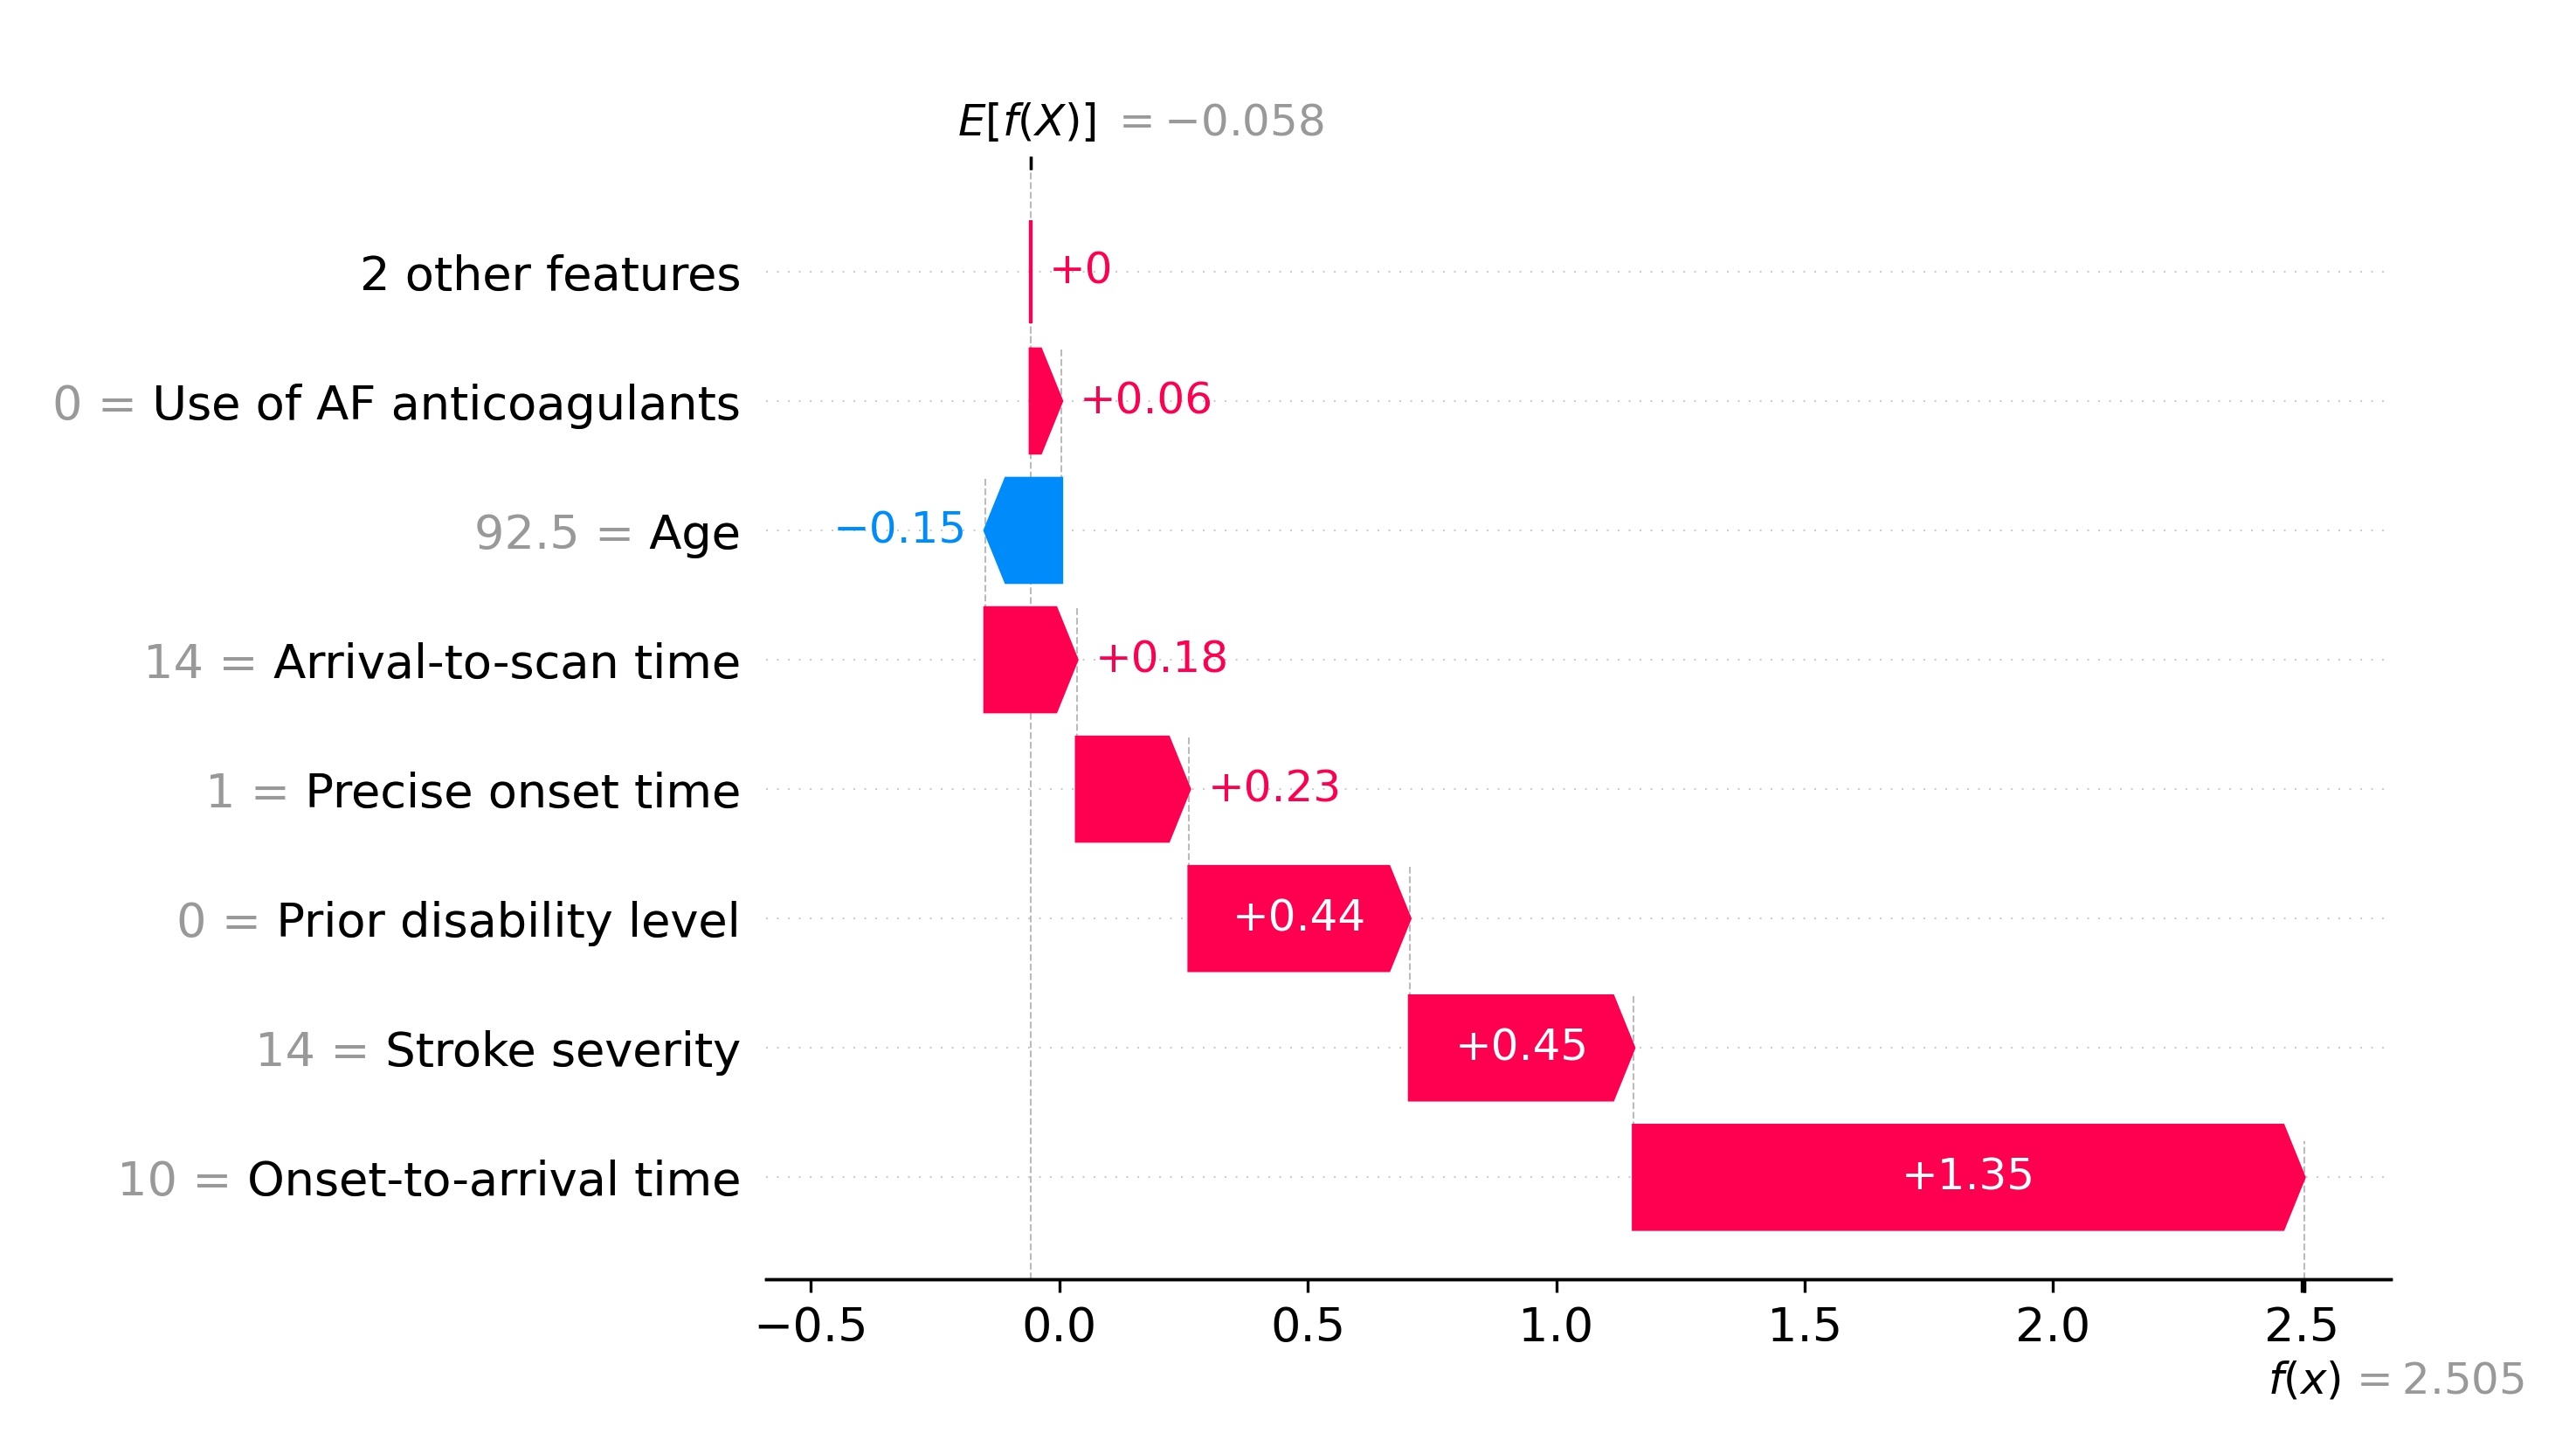
\includegraphics[width=\textwidth]{images/p2_waterfall_odds.jpg}
        \caption{log odds}
        \label{fig:waterfall_subfig1}
    \end{subfigure}
    \hfill
    \begin{subfigure}[b]{0.48\textwidth}
        \centering
        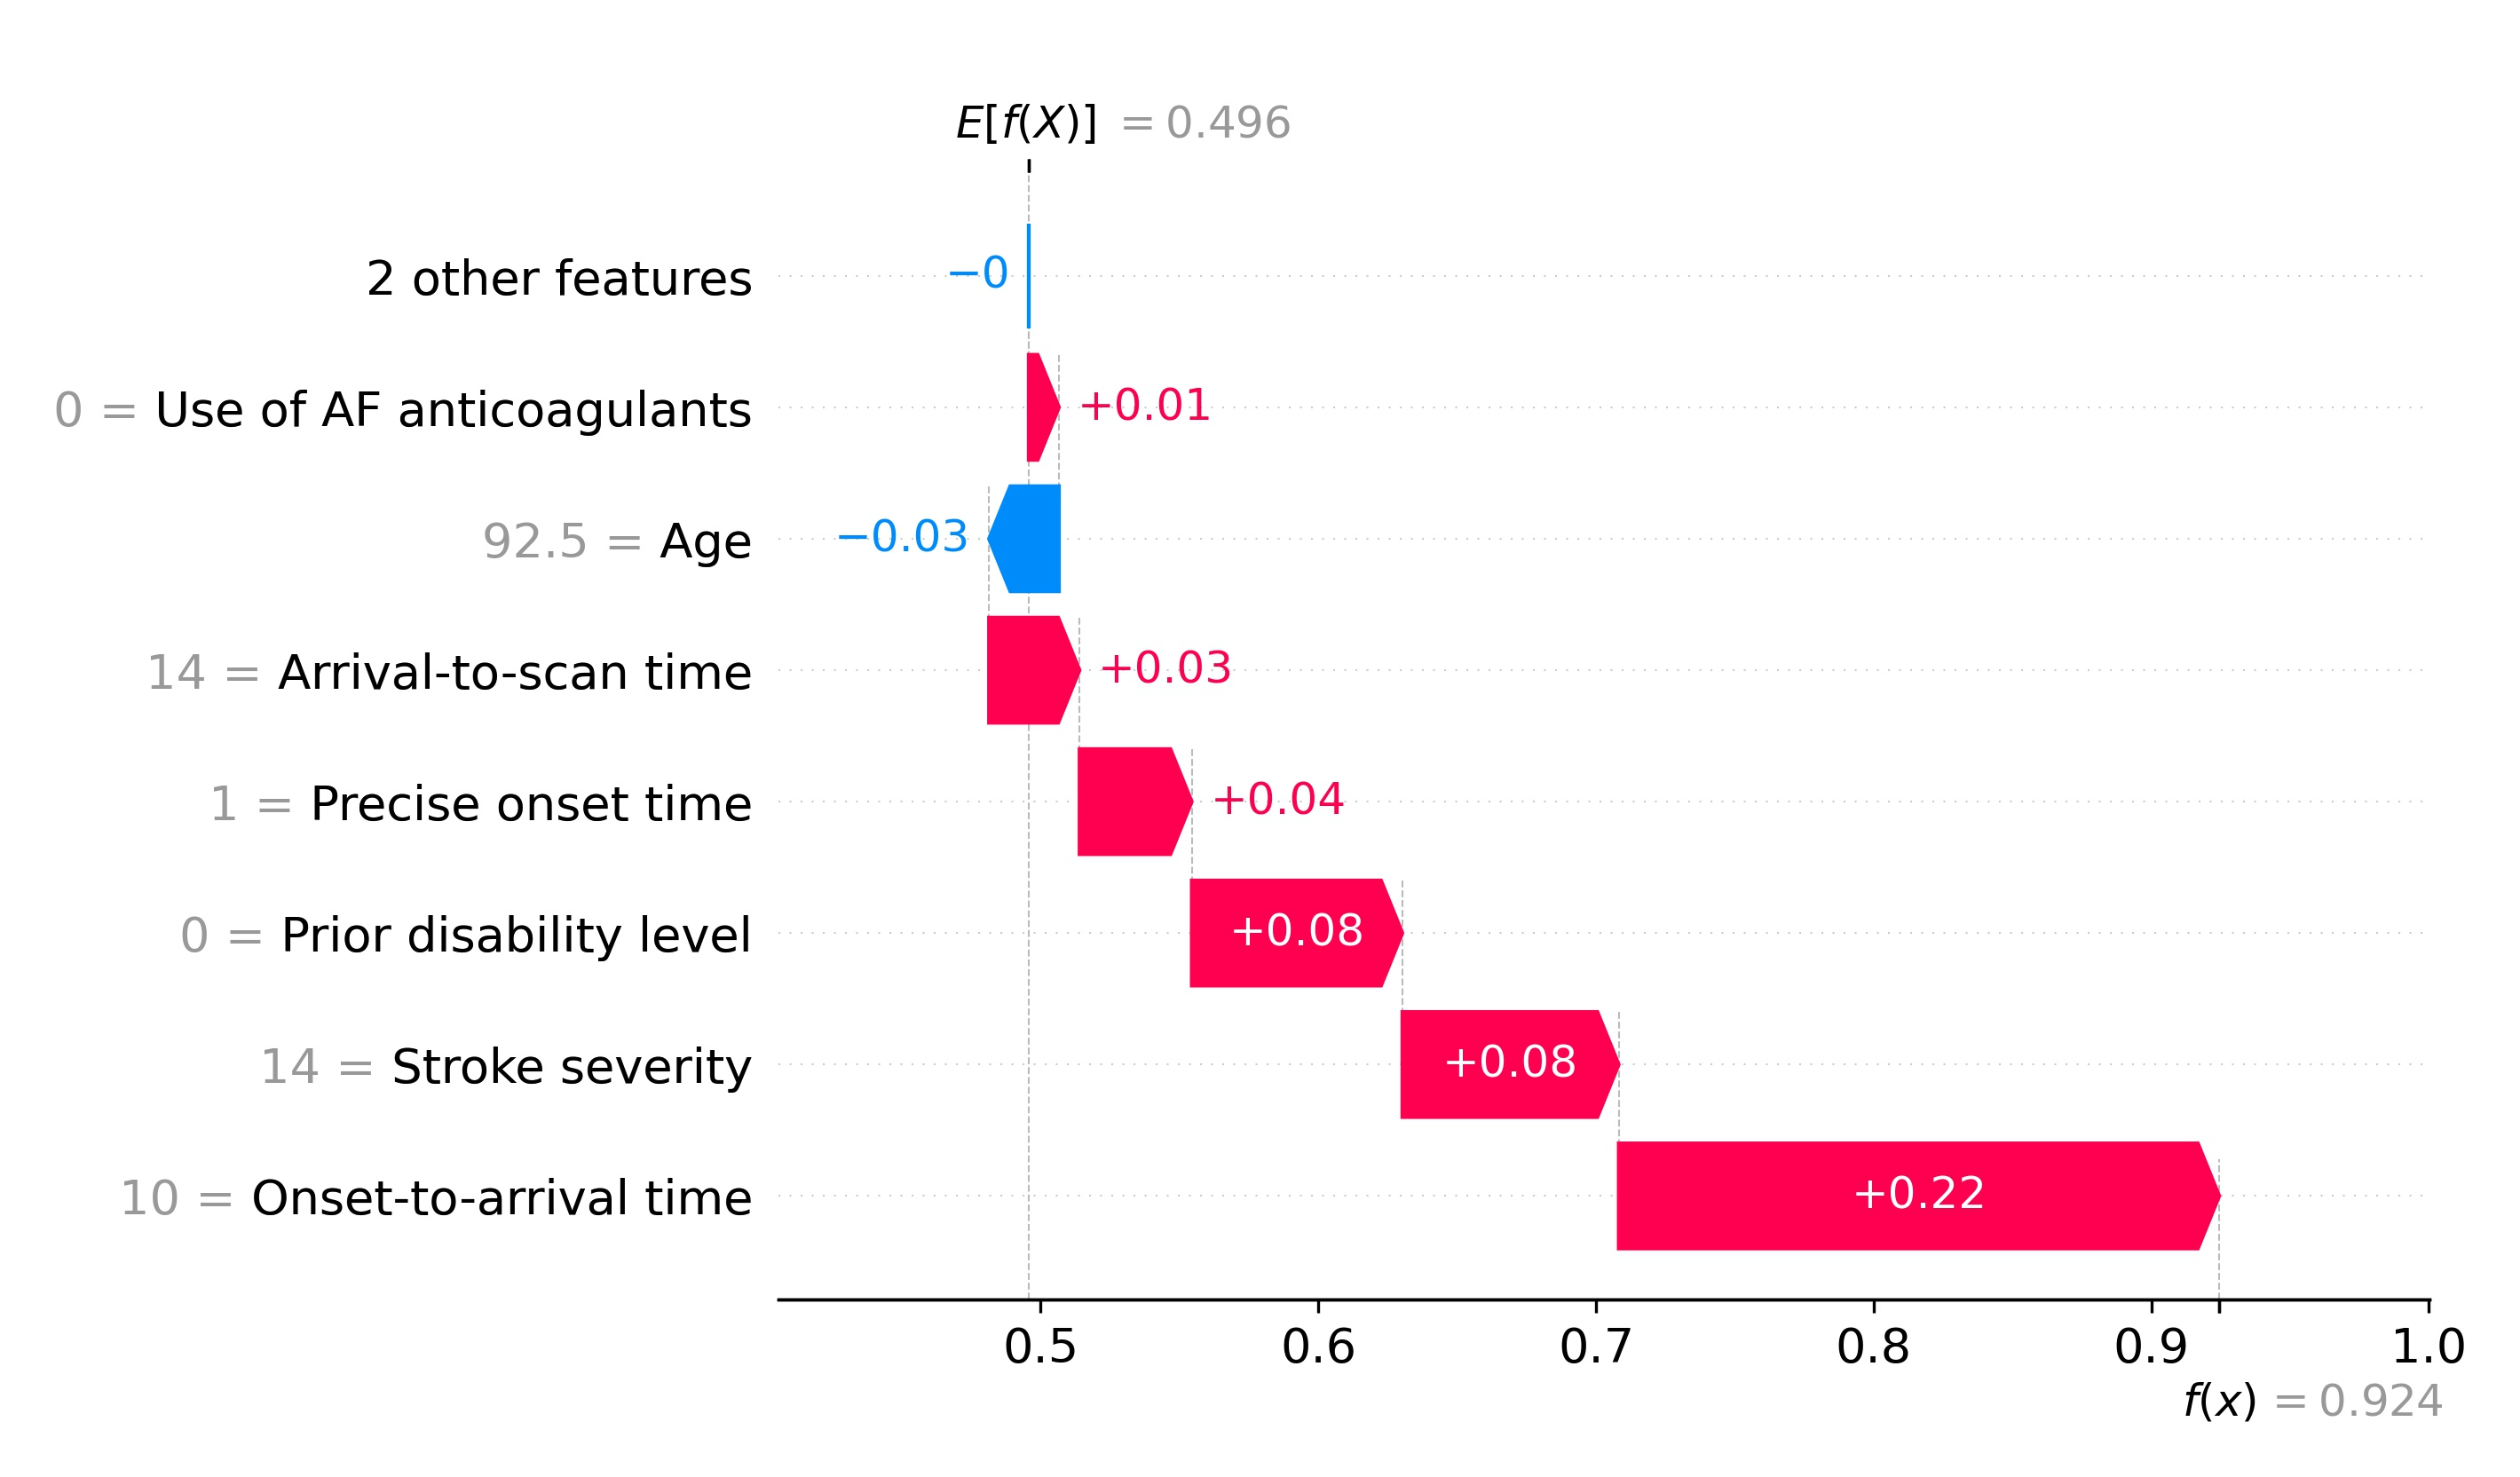
\includegraphics[width=\textwidth]{images/p2_waterfall_probs.jpg}
        \caption{probabilities}
        \label{fig:waterfall_subfig2}
    \end{subfigure}
    \caption{A waterfall plot for an example patient with model prediction and SHAP values expressed either as log odds (left) or probabilities (right). Predictions start with a base value (common to all predictions) of -0.058 log odds or 49.6\% probability of receiving thrombolysis. The individual patient values then contribute to a final prediction of 2.505 log odds or 92.4\% probability of receiving thrombolysis. The most influential features, all increasing the odds of receiving thrombolysis were no prior disability, a severe stroke (NIHSS 14), and 10 minutes onset-to-arrival time.}
    \label{fig:waterfall}
\end{figure}

\subsubsection{Global patterns of patient factors affecting use of thrombolysis}

Global patterns of how feature values affect the odds of receiving thrombolysis are constructed by combining all individual patient prediction SHAP values for each feature.


\begin{figure}
    \centering
    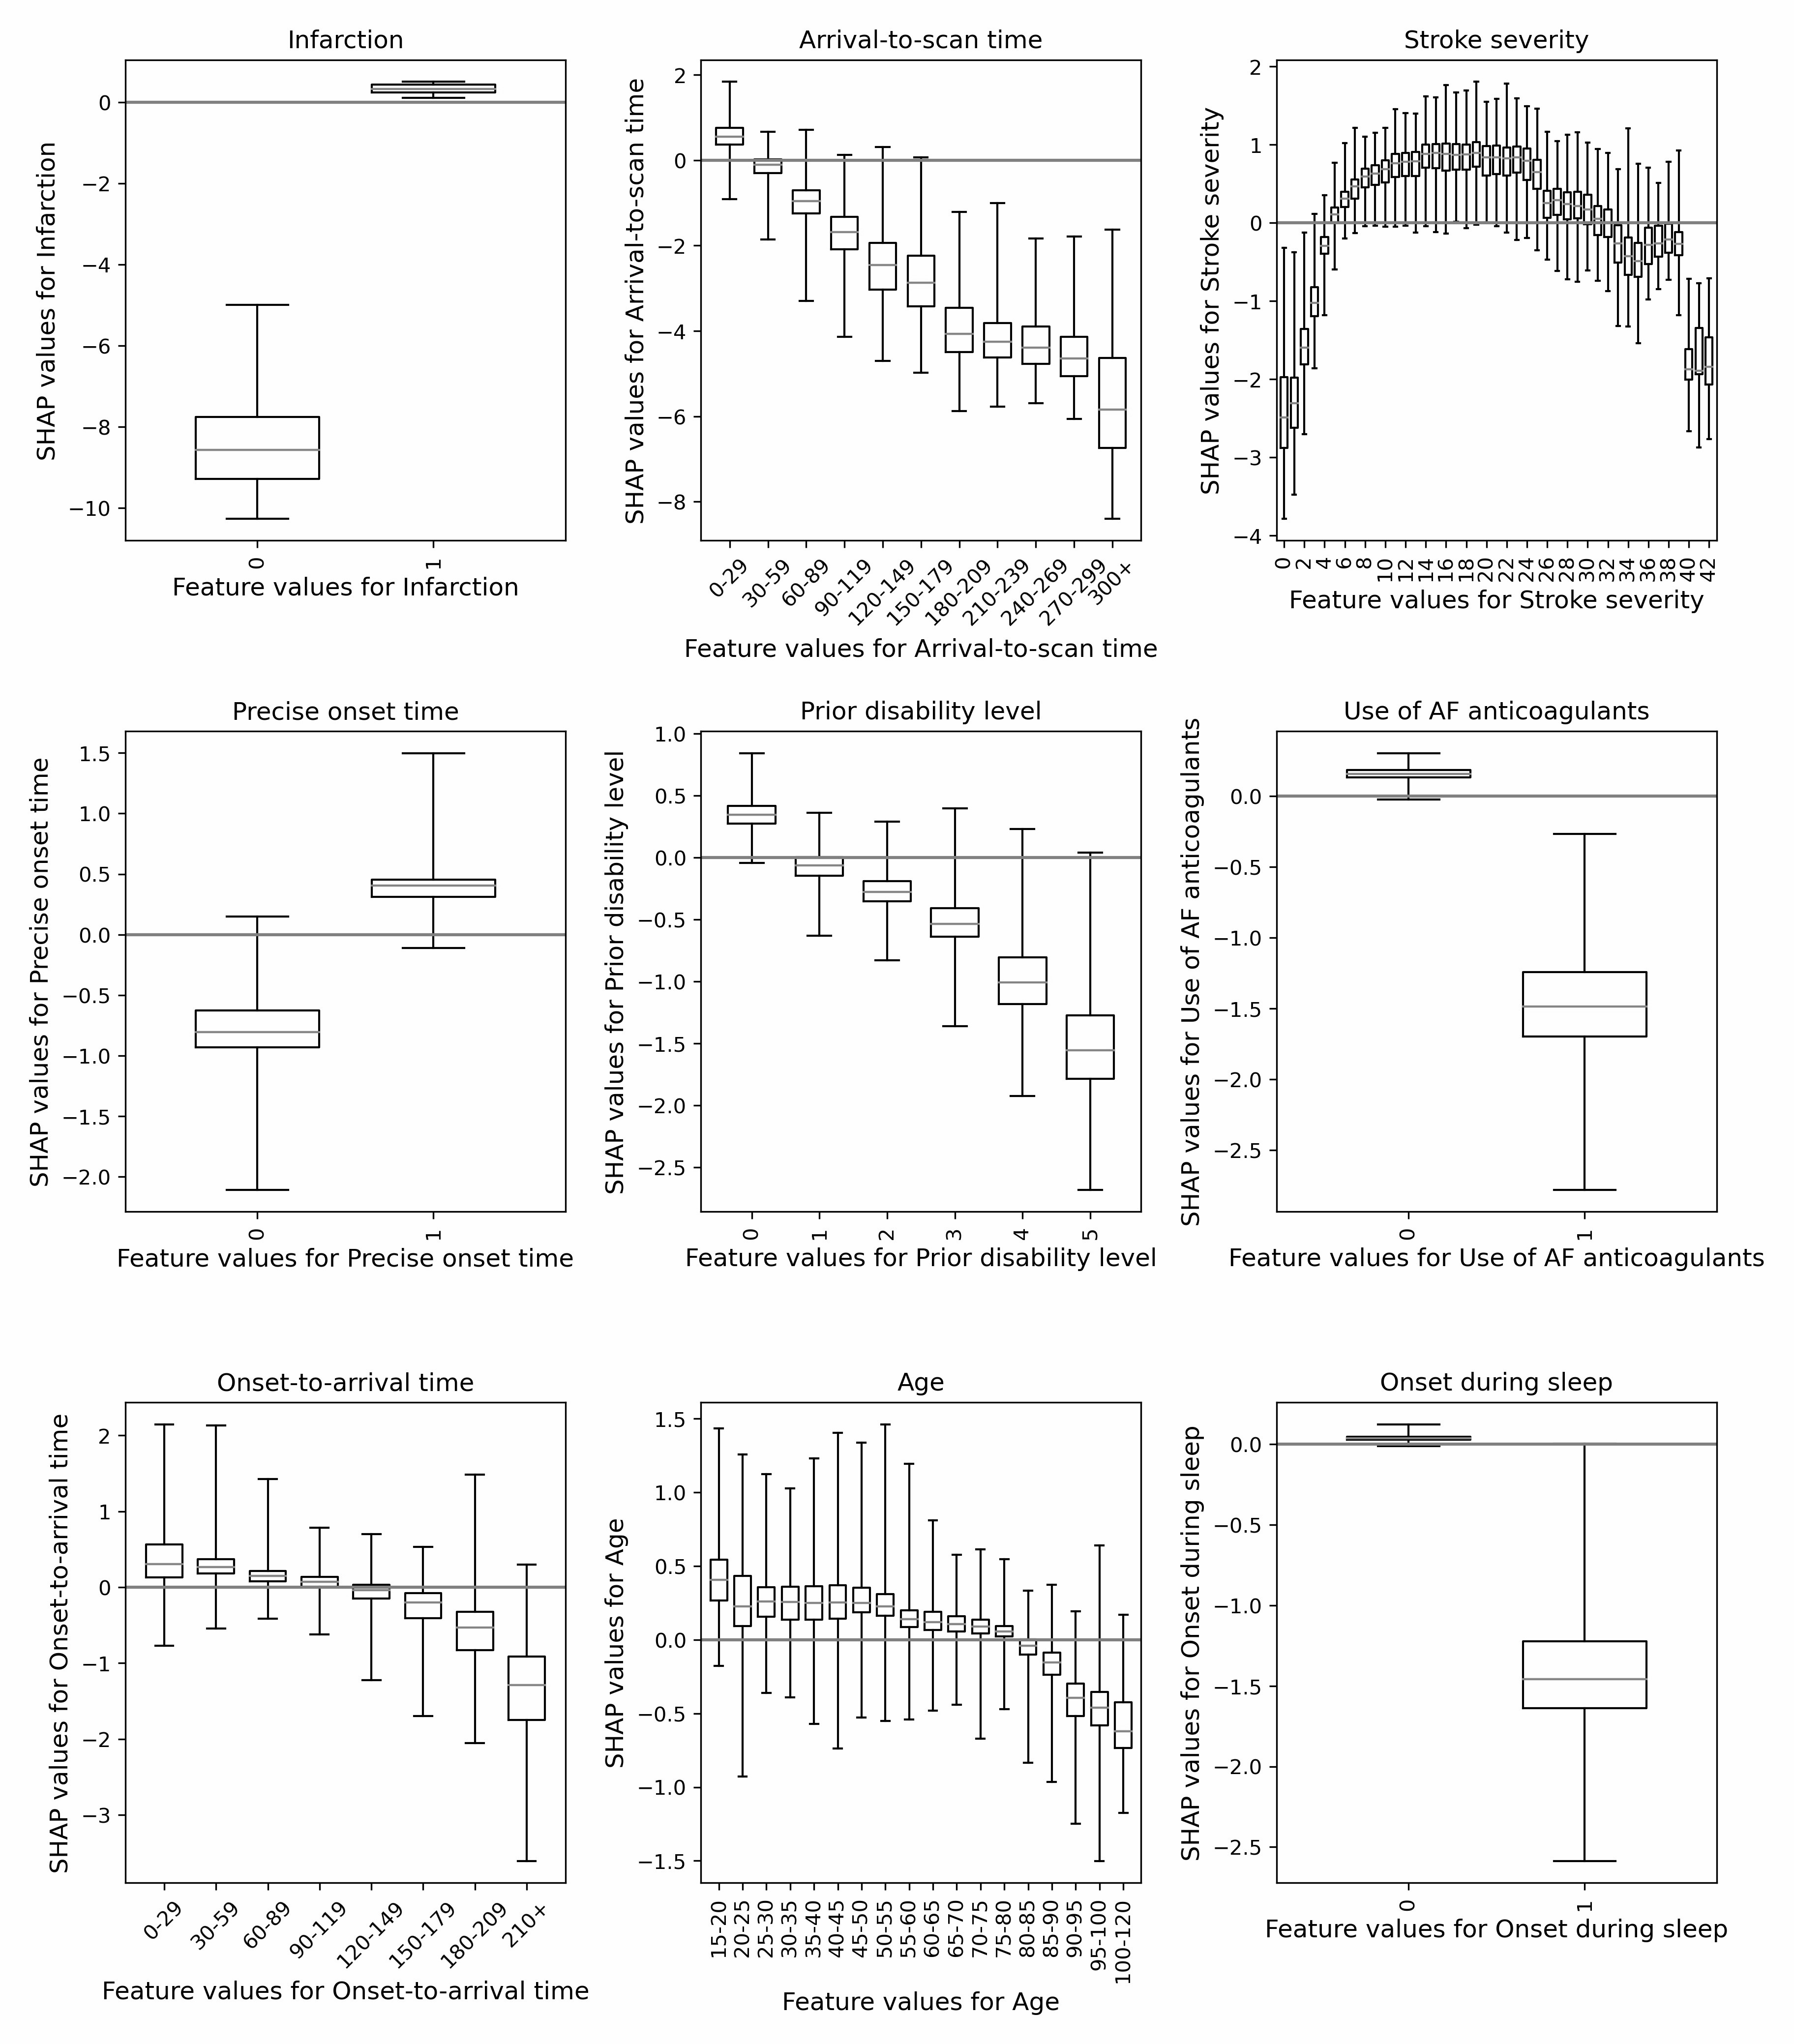
\includegraphics[width=1\linewidth]{images/p2_patient_shap.jpg}
    \caption{Box plots showing the relationship between SHAP values and feature values. Box plots show inter-quartile range (box), median (mid-line in box), and range (whiskers). The plots are ordered in ranked feature importance (using the mean absolute SHAP value across all instances)}
    \label{fig:global_shap}
\end{figure}


Figure \ref{fig:global_shap} shows the relationship between patient characteristics and the log odds of receiving thrombolysis.

Key observations are (with SHAP influence converted from log-odds to odds):

\begin{itemize}
    \item \emph{Stroke type}: The SHAP values for stroke type show that the model effectively eliminated any probability of receiving thrombolysis for non-ischaemic (haemorrhagic) stroke, with the odds of receiving thrombolysis falling by over 6,000 fold.
    \item \emph{Arrival-to-scan time}: The odds of receiving thrombolysis reduced by about 9 fold over the first 120 minutes of arrival-to-scan time.
    \item \emph{Stroke severity (NIHSS)}: The odds of receiving thrombolysis were lowest at NIHSS 0, increased and peaked at NIHSS 15-25, and then fell again with higher stroke severity (NIHSS above 25). The difference between minimum odds (at NIHSS 0) and maximum odds (at 15-25) of receiving thrombolysis was 25-30 fold.
    \item \emph{Stroke onset time type (precise vs. estimated)}: The odds of receiving thrombolysis were about 3 fold greater for precise onset time than estimated onset time.
    \item \emph{Disability level (mRS) before stroke}: The odds of receiving thrombolysis fell about 6 fold between mRS 0 and 5.
    \item \emph{Use of AF anticoagulants}: The odds of receiving thrombolysis were about 5 fold greater for no use.
    \item \emph{Onset-to-arrival time}: The odds of receiving thrombolysis were similar below 120 minutes, then fell about 3 fold between 120 and 240 minutes.
    \item \emph{Age}: The odds of receiving thrombolysis were similar below 80 years old, then fell about 2 fold between 80 and 110 years old.    
    \item \emph{Onset during sleep}: The odds of receiving thrombolysis were about 4 fold lower for onset during sleep.
\end{itemize}

\subsubsection{How hospital attended affects the odds of receiving thrombolysis}

Figure \ref{fig:hospital_shap} shows the distribution of SHAP values for hospital attended. The hospital SHAP value isolates the affect that attending any given hospital has on the odds of receiving thrombolysis. There was a 13 fold difference in odds of receiving thrombolysis between hospitals.

\begin{figure}
    \centering
    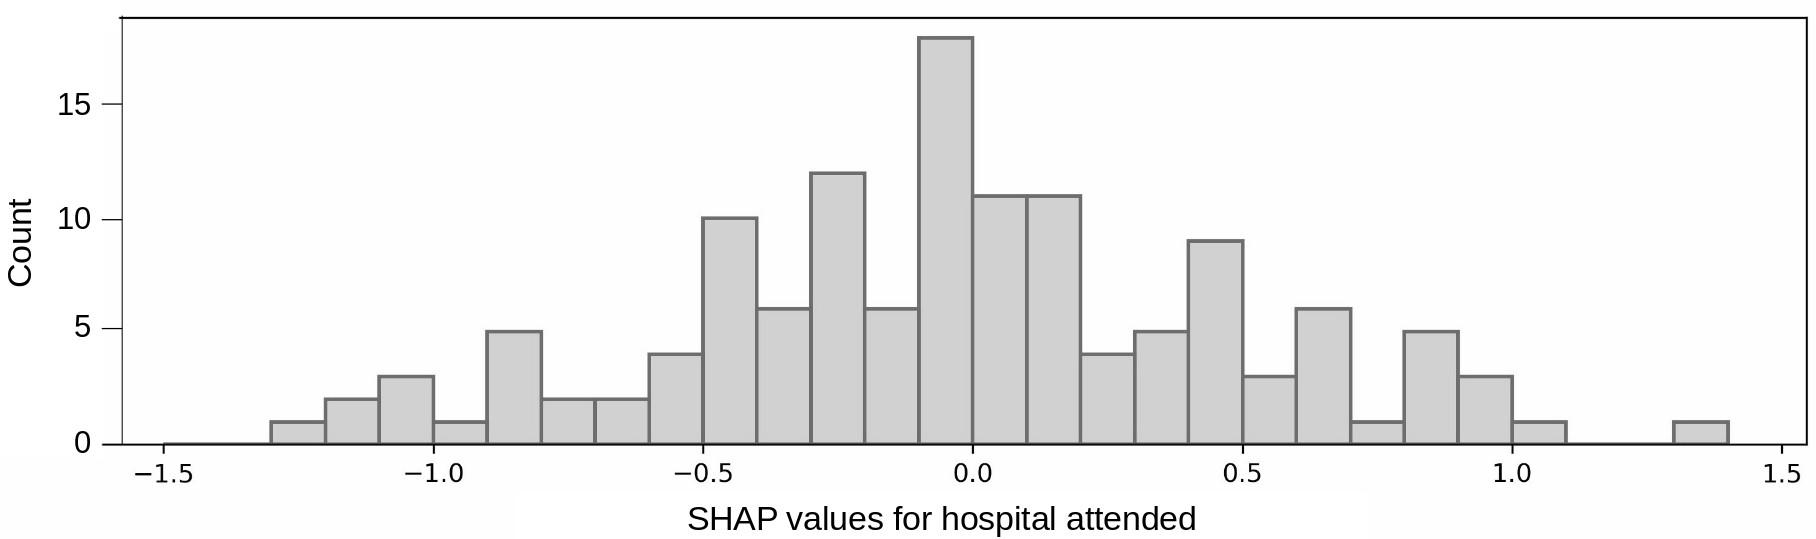
\includegraphics[width=1\linewidth]{images/p2_hosp_shap.jpg}
    \caption{Histogram showing the frequency of SHAP values for the hospital attended.)}
    \label{fig:hospital_shap}
\end{figure}

Overall we found 36\% of the variance in observed between-hospital thrombolysis use can be explained by the patient population characteristics (age, stroke severity, prior disability, onset-to-arrival time, stroke type, type of onset time, anticoagulants, and onset during sleep), 74\% can be explained by hospital identity and processes (arrival-to-scan time, and hospital attended), and that 95\% can be explained by the combined information from both the patient population and hospital identity and processes.

\subsection{Conclusions}

Using explainable machine learning, we have identified how patient features and hospital attended influence decisions to treat with thrombolysis. We showed that the majority of the between-hospital variation in thrombolysis use in England and Wales, for patients arriving with time to thrombolyse, may be explained by differences in in-hospital processes and differences in attitudes to judging suitability for thrombolysis.
% Paper order changed back. The original order first etsablished thrmbolysis works as expected, then goes on to analyse who is receiving it. So paper 3 (clinical trial) supoports paper 4 (rather than vice versa).

\section{Paper 3 highlights: Thrombolysis: Are the results from the clinical trial meta-analysis seen in real life outcomes?  A machine learning study of the UK stroke registry.\cite{pearn_thrombolysis_2024}}\label{sec:paper_3}

\subsection{Objective}

To investigate, using explainable machine learning, the benefit of thrombolysis, and to compare the relationship between time-to-treatment and effectiveness with clinical trial results.

\subsection{Methods overview}

Data for a total of 168,347 ischaemic stroke patients who attended one of 118 emergency stroke hospitals in England and Wales from 2016 to 2021 were extracted from the Sentinel Stroke National Audit Programme (SSNAP). We used explainable machine learning (XGBoost\cite{chen_xgboost_2016} with SHAP\cite{lundberg_unified_2017}) to examine the effect of patient characteristics, hospital attended, and use/time of thrombolysis on the odds of achieving a good outcome (being at or below any given modified Rankin Scale threshold). A linear regression model was fitted to the estimated effect of onset-to-treatment time on thrombolysis to permit comparison with clinical trial meta-analyses.

Code, and full results, for the machine learning work may be found at \url{https://github.com/samuel-book/thrombolysis_clinical_trials_ml_paper}

\subsection{Key results}

\subsubsection{Feature selection}

Using the results from Pearn \textit{el at}. \cite{pearn_are_2024}, we selected seven features as inputs for the model to predict a patient's likelihood of a good outcome at discharge:

\begin{enumerate}
    % No need for saying coding of Yes/No is 1/0
    \item Prior disability level: Estimated mRS score prior to stroke
    \item Stroke severity: National Institutes of Health Stroke Scale (NIHSS) score on arrival
    \item Stroke team: Stroke team attended (hospital identifier)
    \item Age: Age (as midpoint of 5 year age bands)
    \item Onset to thrombolysis time: Time from onset to receiving thrombolysis (minutes). This was set to 9999 if the patient did not receive thrombolysis.
    \item Atrial fibrillation diagnosis: Patient had a diagnosis of atrial fibrillation, either on arrival or diagnosed during admission
    \item Precise onset time known: Onset time recorded was recorded as being precise time, as opposed to a best estimate (\textit{precise} or  \textit{best estimate})
\end{enumerate}

Code and full results for feature selection may be found at \url{https://github.com/samuel-book/feature_selection_thrombolysis_outcome_ml_paper}

\subsubsection{Model accuracy}

With 7 input features, overall accuracy ranged from 77.6\% to 89.7\% across the six models (standard deviation across the 5 k-folds ranged from 0.001 to 0.002). This represented between 95-98\% of the accuracy that is obtained with all the features as inputs. Receiver Operating Characteristic Area Under Curve (ROC-AUC) ranged from 0.852 to 0.893 across the six models (standard deviation across the 5 k-folds ranged from 0.001 to 0.002).

\subsubsection{Global SHAP patterns}

SHAP values explain the contribution (as the change in log-odds) that each feature value has on the model’s prediction of achieving a good outcome at discharge \cite{lundberg_unified_2017}. SHAP values expressed as log-odds are additive (and so are preferred to probabilities, which are not additive, when examining the contribution of individual features to the final prediction). A SHAP model for each of the six machine learning models was created (one for each threshold of mRS to define a good outcome). To illustrate how to interpret the SHAP value in our case, the target feature with a value of 1 represents a good outcome (being at or below any given mRS threshold), and a value 0 represents a worse outcome (being above any given mRS threshold). A positive SHAP value represents that the corresponding feature value increases the likelihood for that patient having a good outcome, and a negative SHAP value represents that the corresponding feature value reduces the likelihood for that patient having a good outcome. SHAP values can be assessed \textit{locally} at patient level, and \textit{globally} at patient cohort level to understand general patterns of how discharge outcomes differ by each of the patient, pathway, and hospital characteristics.

For each patient in the test set we extracted SHAP values for each feature with its corresponding feature value. Figure \ref{fig:global_shap_mrs1} shows the relationship between feature values and the odds of a patient having a good outcome (mRS 0-1) at discharge (a positive SHAP value contributes to an increased likelihood, and a negative SHAP value contributes to a reduced likelihood). We see that low prior disability, lower stroke severity, younger age, receiving thrombolysis (and receiving it sooner after onset), and having no diagnosis of atrial fibrillation contributed to a patient more likely having a good outcome at discharge. Figure \ref{fig:global_shap_ott} focusses on the feature \textit{onset to thrombolysis time}, and its effect at reaching any disability threshold. As time from onset to treatment increased, the beneficial effect of thrombolysis decayed. For thresholds up to, and including, mRS 3, the median effect of thrombolysis remained positive, compared to not receiving thrombolysis, up until the maximum time of 720 minutes. For thresholds of mRS 4 and upwards, the median effect of thrombolysis became negative at longer onset-to-treatment times. This was especially apparent in how thrombolysis changed the overall odds of survival (mRS 0-5) where the median effect of thrombolysis became negative from about 155 minutes. Later thrombolysis may therefore increase the proportion of patients attaining mRS 0-3, but at the cost of some reduction in overall survival. Earlier thrombolysis improved the odds of survival. Figure \ref{fig:global_shap_hosp} shows the contribution from attending a specific hospital to predicting whether the patient had a good outcome at discharge, for each of the mRS threshold levels used to define a good outcome. As the threshold for having a good outcome becomes more inclusive, the range of the effect of the hospital attended had a reduced contribution on the prediction.


\begin{sidewaysfigure}[!h]
    \centering
    \begin{subfigure}[b]{0.8\textwidth}
      \centering
      
\includegraphics[trim={0 0 0 1.2cm}, clip, width=1\textwidth]{./images/p3_clin_shap_sub_1}\\
      \caption{The relationship between feature values and the prediction of whether a patient will have a good outcome (mRS 0-1) at discharge. SHAP base value for this model is -1.529.}
      \label{fig:global_shap_mrs1}
    \end{subfigure}
    \hfill
    \begin{subfigure}[b]{0.8\textwidth}
      \centering    
      
\includegraphics[width=1\textwidth]{./images/p3_clin_shap_sub_2.jpg}\\
%      \includegraphics[trim={0 0 0 1.2cm}, clip, width=1\textwidth]{./images/083_xgb_7_features_5fold_binary_shap_violin_ss_0kfold}\\
      \caption{The relationship between onset to thrombolysis time and the prediction of whether a patient will have a good outcome at discharge, for each of the mRS scores used to define a good outcome.}
      \label{fig:global_shap_ott}
    \end{subfigure}
    \hfill
    \begin{subfigure}[b]{0.8\textwidth}
      \centering
      
\includegraphics[trim={0 0 0 1.2cm}, clip, width=1\textwidth]{./images/p3_clin_shap_sub_3}\\
      \caption{The contribution from attending a specific hospital to predicting whether the patient will have a good outcome at discharge, for each of the mRS scores used to define a good outcome}
      \label{fig:global_shap_hosp}
    \end{subfigure}
    \label{fig:global_shap_trio}
  \caption{The relationship between feature values SHAP values in predicting whether a patient will have a good outcome. Violin plots show the distribution of SHAP values across the patient population for each feature value, with the mid-line showing the median SHAP value.} 
\end{sidewaysfigure}

%\FloatBarrier


\subsubsection{The direct contribution of thrombolysis use to the shift in probability of a good outcome}

We used the first k-fold train/test set split (4:1 train:test data) to investigate likely outcome from thrombolysis. For each patient in the test set that received thrombolysis within 300 minutes from stroke onset (n = 6,796), we performed a counterfactual analysis, predicting outcome probabilities if the patient had not received thrombolysis. We calculated the effect of thrombolysis by taking the difference in SHAP values, between treated and the predicted outcome if untreated, for the contribution of thrombolysis to achieving a good outcome.

We modelled the decay in effect of thrombolysis by fitting a linear regression model to the benefit of thrombolysis (log odds shift in attaining a good outcome) with time from onset to treatment (excluding patients treated after 300 minutes). The model used the definition of mRS 0-1 as a good outcome to match the definition used in the meta-analysis of clinical trials \cite{emberson_effect_2014}. The analysis was applied to three patient cohorts: (1) all treated ischaemic strokes (n = 6,796), (2) treated severe ischaemic strokes, NIHSS 11+ (n = 2,856), (3) treated mild-moderate ischaemic strokes, NIHSS 0-10 (n = 3,940). 

Figure \ref{fig:linear_regression_plots} shows a linear regression fitted to the shift in the contribution from receiving thrombolysis towards having a good outcome at discharge (mRS 0-1) with respect to the onset to thrombolysis time. We found, for all treated patients, that the effect of thrombolysis had declined to zero at 328 minutes, and the effect from thrombolysis was improving log odds of a good outcome by 0.90 if it were, theoretically, given at the time of stroke onset. We observed that the maximum theoretical effect of thrombolysis (if given at time of stroke onset) was greater for the severe stroke group (1.048 log odds) than the mild-moderate stroke group (0.771 log odds). However the effect of thrombolysis declined a little faster in the severe stroke group (reaching no effect at 314 minutes for severe stroke patients, compared to 351 minutes for mild-moderate stroke patients). Linear regression coefficients in all three patient groups were statistically significant (table \ref{fig:stats_table_mrs1}). 

\begin{figure}[h]
    \centering
    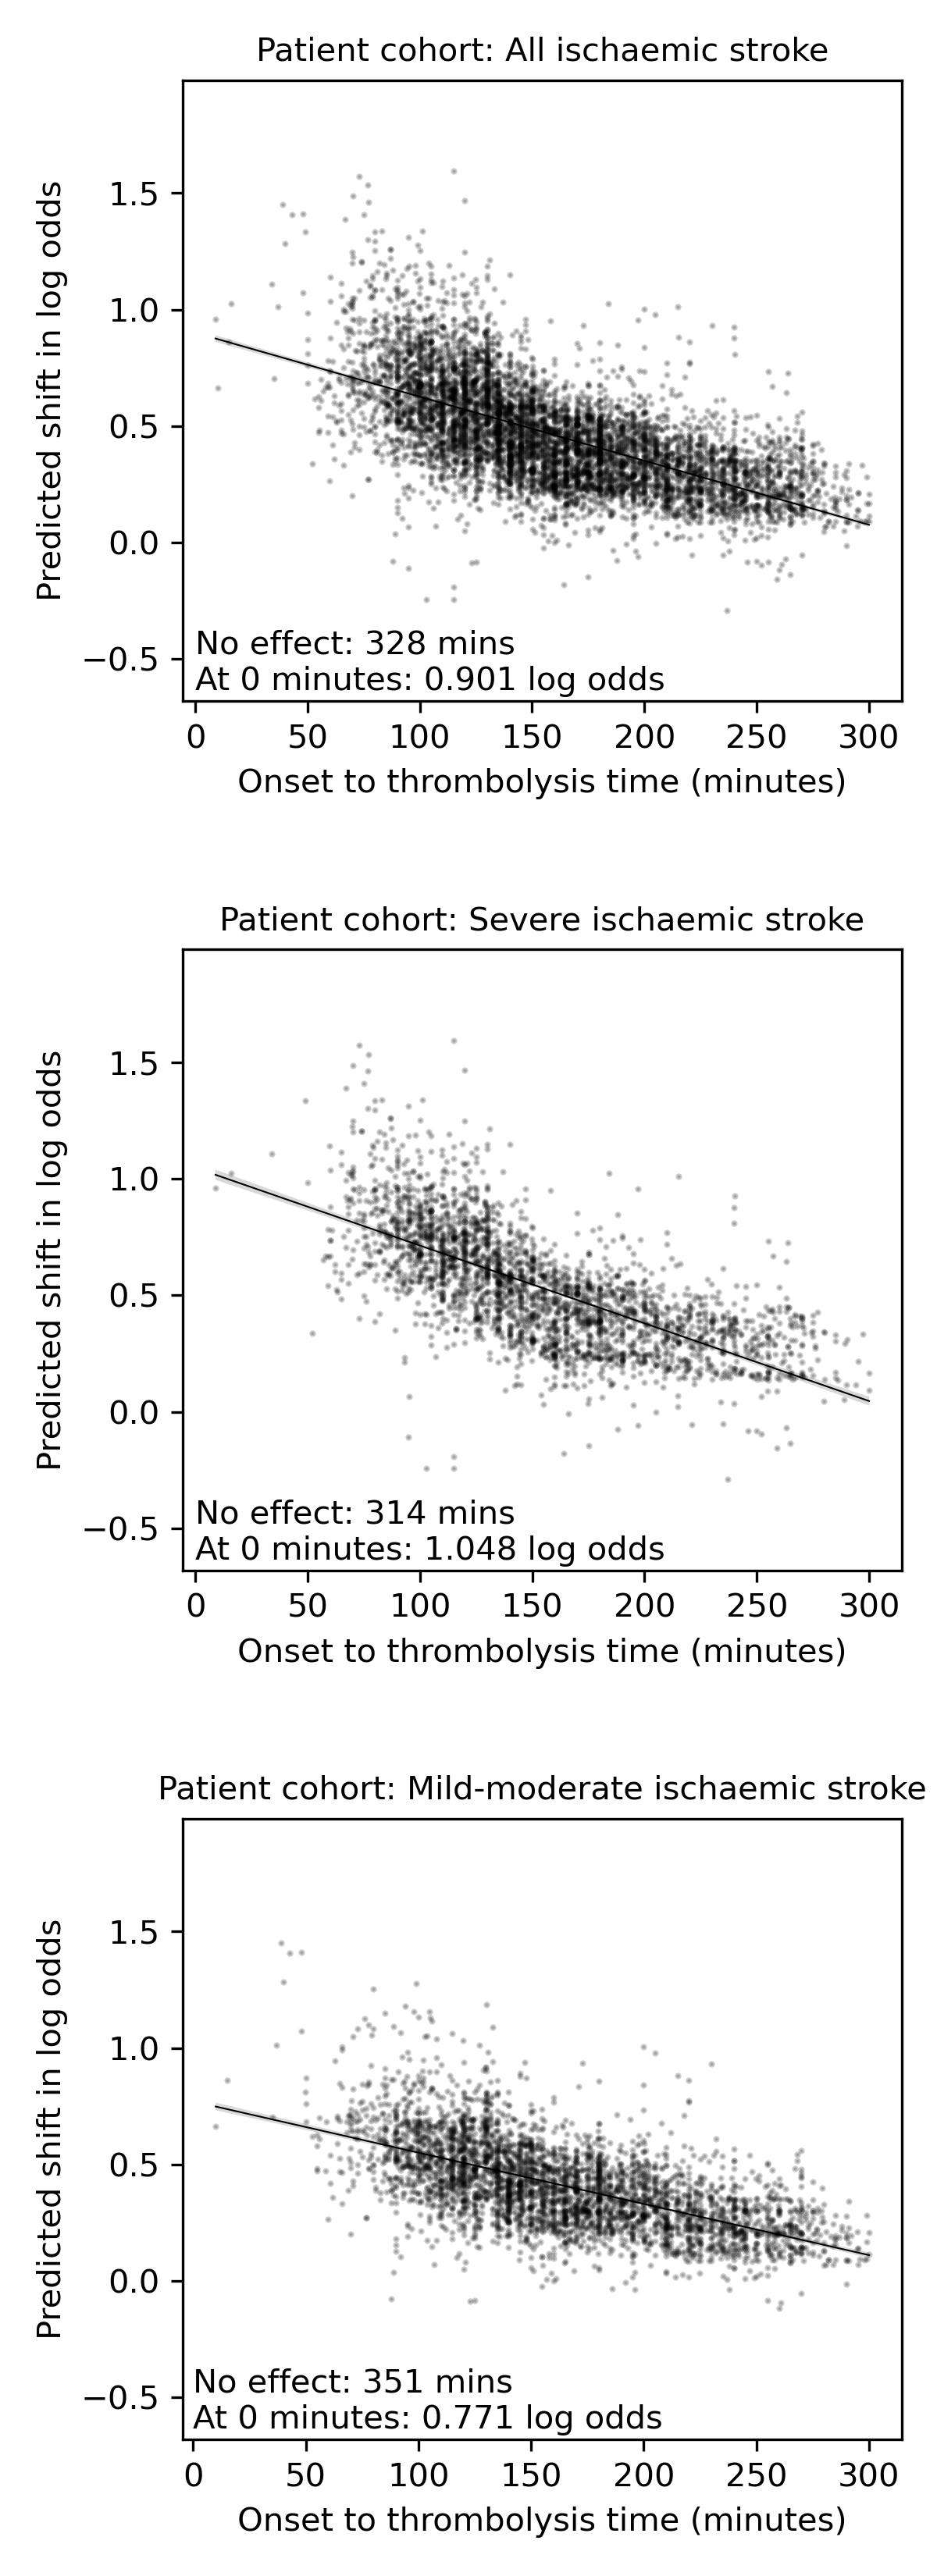
\includegraphics[width=0.40\textwidth]{./images/p3_regression_v1}\\
    \caption{A linear regression fit to the contribution from receiving thrombolysis in having a good outcome (mRS 0-1) at discharge, with respect to the onset to thrombolysis time (for patients treated within 300 minutes). Top: all treated stroke patients (n = 6,796); Middle: treated severe stroke patients, NIHSS 11+ (n = 2,856); Bottom: treated mild-moderate stroke patients, NIHSS 0-10 (n = 3,940).}
    \label{fig:linear_regression_plots}
\end{figure}

\begin{table}
    \caption{Fitting linear regression to the shift in the contribution from receiving thrombolysis towards having a good outcome (mRS 0-1) at discharge with respect to the onset to thrombolysis (OTT) time. Linear regression statistics for different patient cohorts. We used NIHSS 0-10 to define mild-moderate strokes, and NIHSS 11+ to define severe strokes.}
    \centering
        \begin{tabular}{lllllllll}
        \toprule
         Ischaemic stroke type & Variables & coef & std err & t & P$>$$|$t$|$ & [0.025 & 0.975] \\ 
         \midrule
        All & Constant & 0.9012 & 0.007 & 132.519 & 0.000 & 0.888 & 0.915\\
        & OTT time (min) &  -0.0027  & 4.04e-05 & -68.058 & 0.000 & -0.003 & -0.003\\   
        \midrule
        Severe & Constant & 1.0476  &    0.011  & 96.746 & 0.000 & 1.026 & 1.069\\
        & OTT (mins) & -0.0033 &  6.67e-05  & -50.042 & 0.000 & -0.003 & -0.003\\ 
        \midrule
        Mild-moderate & Constant &           0.7708 &     0.008   & 97.613 & 0.000 & 0.755 & 0.786\\
        & OTT time (mins) &  -0.0022 &   4.57e-05 & -48.109 & 0.000 & -0.002 & -0.002\\
        \bottomrule
        \end{tabular}
      \label{fig:stats_table_mrs1}
\end{table}

\subsection{Conclusions}

Using machine learning methods with SHAP in a very large prospective national stroke registry, thrombolysis was found to be associated with a statistically significant improvement in the odds of having a good outcome using any mRS threshold. Regression analysis predicted a maximum 2.5-fold improvement in odds of achieving mRS 0-1, with a decline to no treatment effect at 5 hours 28 minutes post-onset. The findings from this study were remarkably similar to the meta-analysis of clinical trials 8, which extrapolate back to a 0.69 log odds (equivalent to an odds ratio of 2.0) improvement of being mRS 0-1 at stroke onset, with no effect after 6 hours 18 minutes.
% Paper order changed back. The original order first etsablished thrmbolysis works as expected, then goes on to analyse who is receiving it. So paper 3 (clinical trial) supoports paper 4 (rather than vice versa).

\section{Paper 4 highlights: Are the patients who would benefit from thrombolysis the same ones as those receiving it? A machine learning study of the UK stroke registry.\cite{pearn_are_2024}}\label{sec:paper_4}

\subsection{Objective}

To investigate, using explainable machine learning, the overlap and differences between the groups of patients receiving thrombolysis, and the group of patients predicted to benefit from thrombolysis.

\subsection{Methods overview}

\subsubsection{Outcome prediction}

Data for a total of 78,396 ischaemic stroke patients who attended one of 111 emergency stroke hospitals in England and Wales and had brain imaging within 255 minutes of stroke onset, from 2016 to 2021, were extracted from the Sentinel Stroke National Audit Programme (SSNAP). We used explainable machine learning (XGBoost\cite{chen_xgboost_2016} with SHAP\cite{lundberg_unified_2017}) to examine the effect of patient characteristics, hospital attended, and use/time of thrombolysis on the patients’ predicted outcome (modified Rankin Scale, mRS) at discharge. The data excludes patients on anticoagulants for atrial fibillation (representing 12.9\% of the population) as these patients may be at risk of adverse outcome that is not predicted by the machine learning model (as it is likely thrombolysis is only given to patients on anticoagulants when when it has been shown that blood clotting is normal).

The model predicts probability of each mRS category outcome. \textit{Probability-weighted mRS} was used as a measure of the mid-point location of disability; it is the sum of each mRS outcome multiplied by the probability of that outcome occurring

We predicted the expected effect of thrombolysis for all patients, and compared who would benefit from thrombolysis with those who actually received thrombolysis. We used a conservative definition to determine whether a patient would likely have a better outcome with treatment from the two probability distributions, where both of these criteria must be met: 

\begin{enumerate}
    \item a reduction in probability-weighted mRS, \textbf{and}
    \item a reduction in the likelihood of a very bad outcome (mRS 5-6, complete dependency or death).
\end{enumerate}

\subsubsection{Hospital trade-off between maximising benefit from thrombolysis and minimising risk of harm from thrombolysis}

We trained a separate XGBoost \textit{thrombolysis decision} model, to predict the likelihood of a patient receiving thrombolysis, using methods previously described \cite{pearn_what_2023}. We used this to predict likely thrombolysis use for all patients at all stroke teams. This was used to compare likely decision-making and outcomes across if all stroke teams saw the same patients. To compare maximising benefit from thrombolysis and avoiding potential harm from thrombolysis we defined measures for \textit{sensitivity} and \textit{specificity} of treatment. \textit{Sensitivity} was calculated as the proportion of patients who were predicted to benefit from thrombolysis (from the \textit{thrombolysis outcome} model) who were predicted to receive thrombolysis at each team (from the \textit{thrombolysis decision} model). \textit{Specificity} was calculated as the proportion of patients who were predicted not to benefit from thrombolysis (from the \textit{thrombolysis outcome} model) who were not predicted to receive thrombolysis at each team (from the \textit{thrombolysis decision} model). A low \textit{sensitivity} would indicate a higher likelihood of not treating people who would benefit from thrombolysis, and a low \textit{specificity} would indicate a higher likelihood of treating people who would not benefit from thrombolysis.

Code, and full results, for the machine learning work may be found at \url{https://github.com/samuel-book/thrombolysis_outcome_ml_paper}.

\subsection{Key results}

\subsubsection{Feature selection}

We selected seven features as inputs for the model to predict a patient's likelihood of a good outcome at discharge:

\begin{enumerate}
    \item Prior disability level: Estimated mRS score prior to stroke
    \item Stroke severity: National Institutes of Health Stroke Scale (NIHSS) score on arrival
    \item Stroke team: Stroke team attended (hospital identifier)
    \item Age: Age (as midpoint of 5 year age bands)
    \item Onset to thrombolysis time: Time from onset to receiving thrombolysis (minutes). This was set to 9999 if the patient did not receive thrombolysis.
    \item Atrial fibrillation diagnosis: Patient had a diagnosis of atrial fibrillation, either on arrival or diagnosed during admission (1 = Yes, 0 = No)
    \item Precise onset time known: Onset time recorded was recorded as being precise time, as opposed to a best estimate (1 = precise, 0 = best estimate)
\end{enumerate}

Code and full results for feature selection may be found at \url{https://github.com/samuel-book/feature_selection_thrombolysis_outcome_ml_paper}

\subsubsection{Model accuracy}

Receiver Operating Characteristic Area Under Curve (ROC-AUC) was 0.796 (0.001 standard deviation across the 5 k-folds). Classification accuracy across the seven mRS outcomes was 41.1\% (0.002 standard deviation across the 5 k-folds). Accuracy to within one mRS category was 72.4\% (0.002 standard deviation across the 5 k-folds).  

\subsection{Comparing actual use of thrombolysis and predicted benefit from thrombolysis}

We used the first k-fold train/test set split (4:1 train:test data) to investigate likely outcome from thrombolysis. In the test set of 15,680 patients, 44\% received thrombolysis. For each patient we predicted outcomes with and without thrombolysis. Figure \ref{fig:scatter_all} shows the expected shift in probability-weighted mRS at discharge, and the change in probability of being discharged with mRS 5-6, due to thrombolysis, separated by whether the patient actually received thrombolysis or not. Overall, 60\% of patients were predicted to benefit from thrombolysis. Of those who did receive thrombolysis, 73\% were predicted to have both a better average disability likelihood and a reduction in probability of being mRS 5-6. 9\% were predicted to have both a worse average disability likelihood and an increase in probability of being mRS 5-6. 18\% were predicted to have either, but not both, a better average disability likelihood or a reduction in probability of being mRS 5-6. Of those who did not receive thrombolysis, 49\% were predicted to have both a better average disability likelihood and a reduction in probability of being mRS 5-6. 26\% were predicted to have both a worse average disability likelihood and an increase in probability of being mRS 5-6. 25\% were predicted to have either, but not both, a better average disability likelihood or a reduction in probability of being mRS 5-6.

\begin{figure}
\centering
\begin{subfigure}{.7\textwidth}
  \centering
  \captionsetup{width=.9\linewidth}
  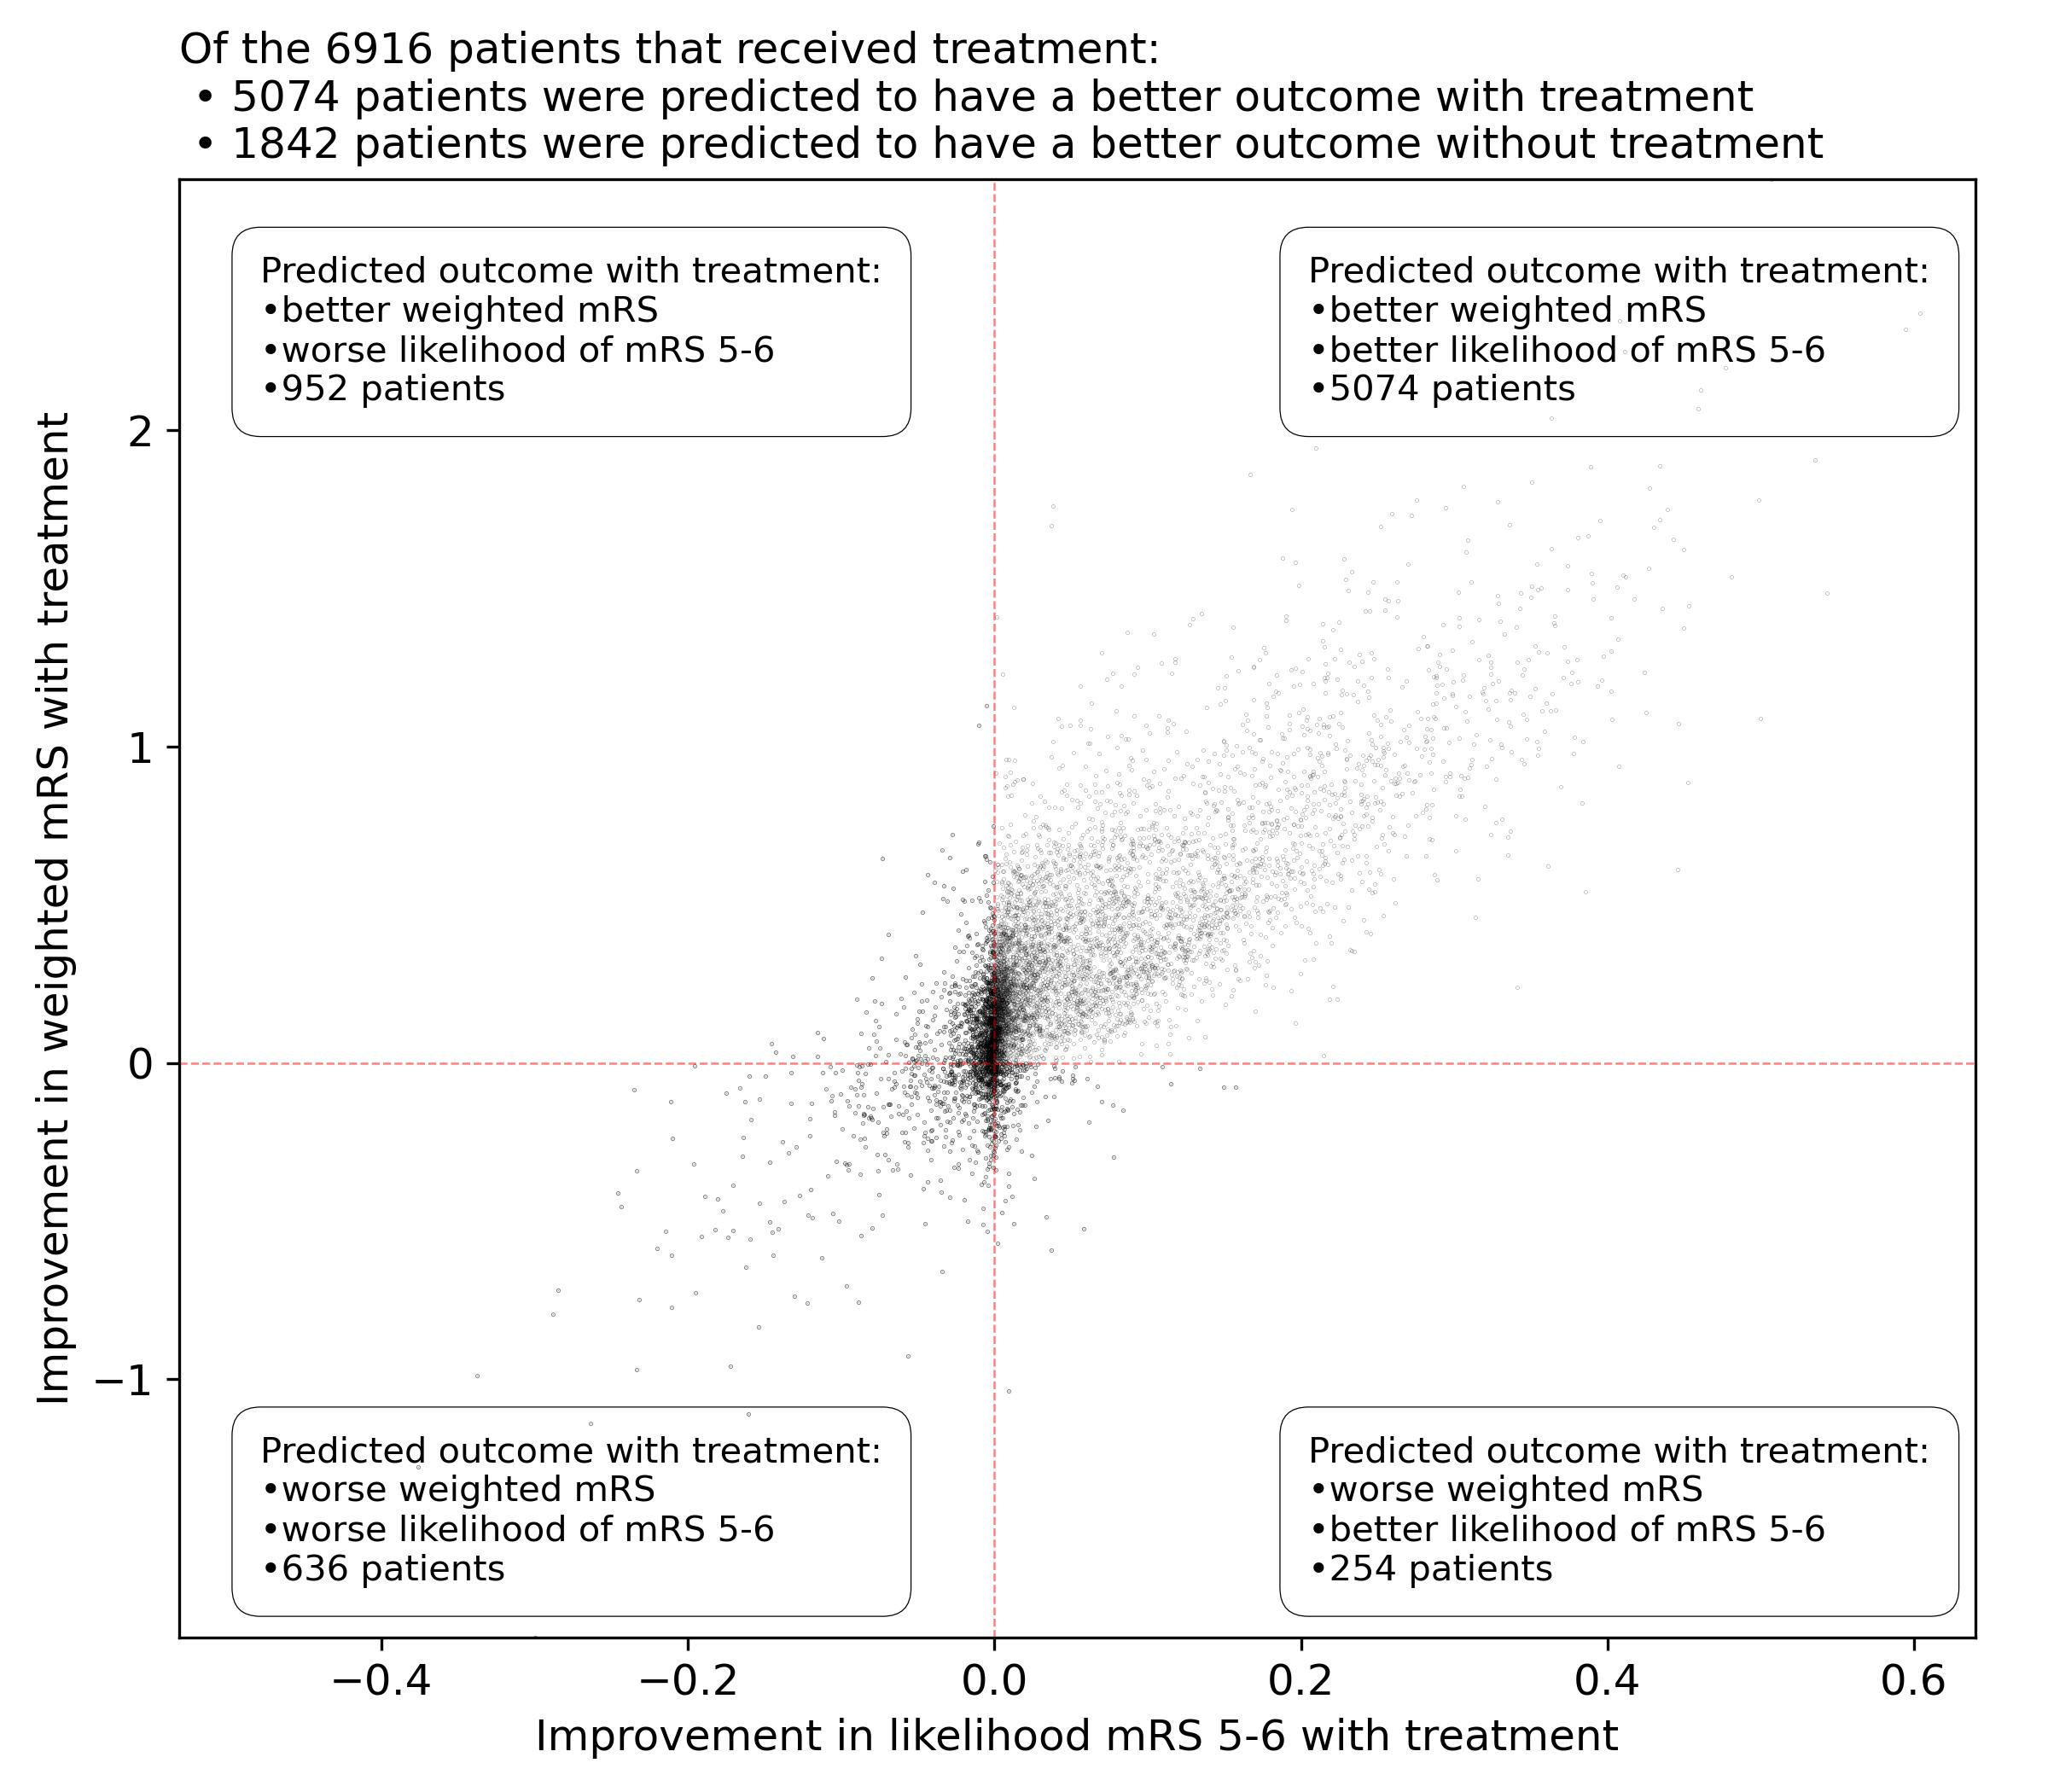
\includegraphics[trim={0 0 0 1.7cm}, clip, width=1\linewidth]{./images/p4_scatter_treated}
  \caption{\footnotesize{Patients who received thrombolysis (n = 6,916)}}
  \label{fig:scatter_receive}
\end{subfigure}

\vspace{5mm}


\begin{subfigure}{.7\textwidth}
  \centering
  \captionsetup{width=.9\linewidth}
  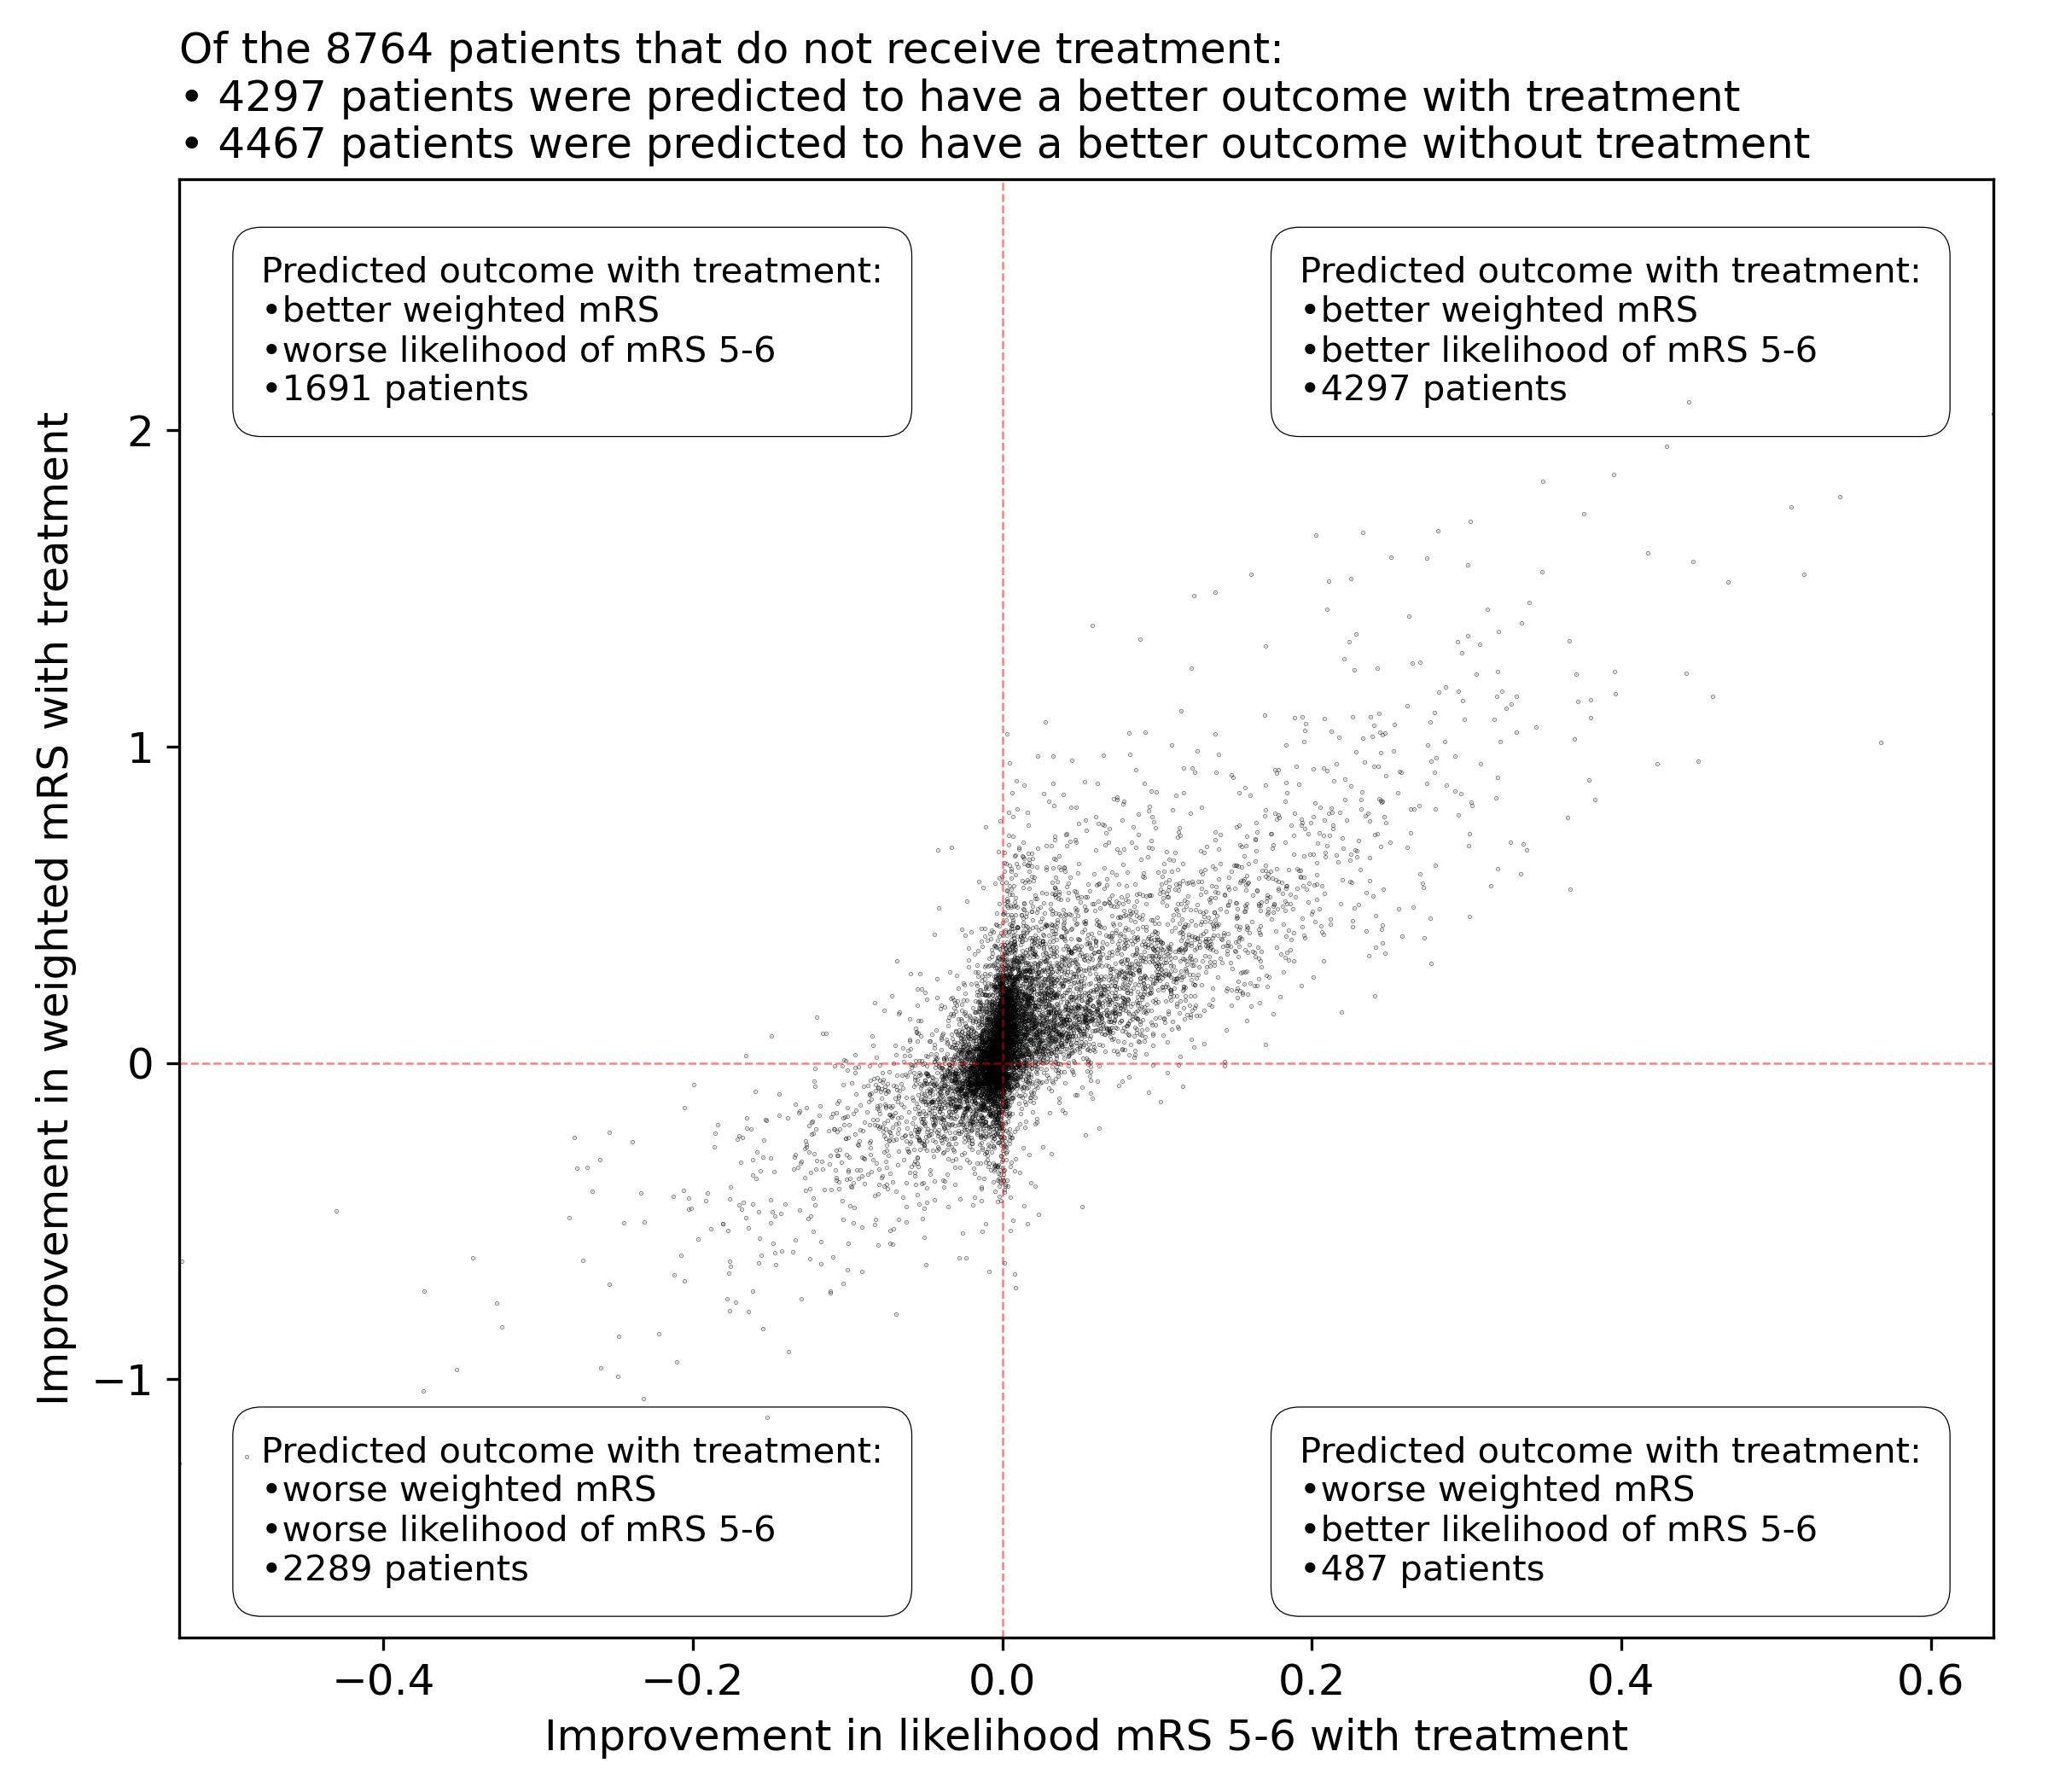
\includegraphics[trim={0 0 0 1.7cm}, clip, width=1\linewidth]{./images/p4_scatter_not_treated}
  \caption{\footnotesize{Patients who did not receive thrombolysis (n = 8,764)}}
  \label{fig:scatter_not_receive}
\end{subfigure}
  \caption{The predicted benefit or disbenefit of thrombolysis for each of the 15,680 patients in the first k-fold test set. Benefit is shown as both the expected improvement in probability-weighted disability (y-axis) and the improvement in likelihood of avoiding discharge with mRS 5-6. Both measures are expressed so that a positive value is better (a reduction in probability-weighted disability or a reduction in probability of discharge with mRS 5-6). (a) Patients who did actually receive thrombolysis (n = 6,916), (b) Patients who did not actually receive thrombolysis (n = 8,764).}
\label{fig:scatter_all}
\end{figure}

\subsection{Patient characteristics that contribute to a mismatch between actual thrombolysis use and predicted best outcome}

We compared the distribution of feature values for two patient cohorts: i) patients that received thrombolysis but were predicted to not have a better outcome with thrombolysis, ii) patients that did not receive thrombolysis but were predicted to have a better outcome with thrombolysis. When examining individual feature values in this way we did not identify any features that could be used in isolation to identify those patients who would benefit from thrombolysis but did not receive thrombolysis (or vice-versa). Patients who received thrombolysis but would likely not benefit from it have a range of feature values for each patient feature, as do those patients who did not receive thrombolysis but would benefit from it.

\subsection{Hospital trade-off between maximising benefit from thrombolysis and minimising risk of harm from thrombolysis}

The XGBoost \textit{thrombolysis decision} model had an accuracy of 78.7\% and ROC-AUC of 0.86. Figure \ref{fig:hosp_shap_scatter} shows the trade-off between the individual hospitals \textit{sensitivity} and \textit{specificity} towards giving treatment. We found that those hospitals attaining a higher predicted \textit{sensitivity} of treatment (not missing patients who would benefit from treatment) also tended to have a lower \textit{specificity} (giving thrombolysis to patients who would likely not benefit from it).

%218_hosp_shap_scatter.png}}\\

\begin{figure}
    \centering
    {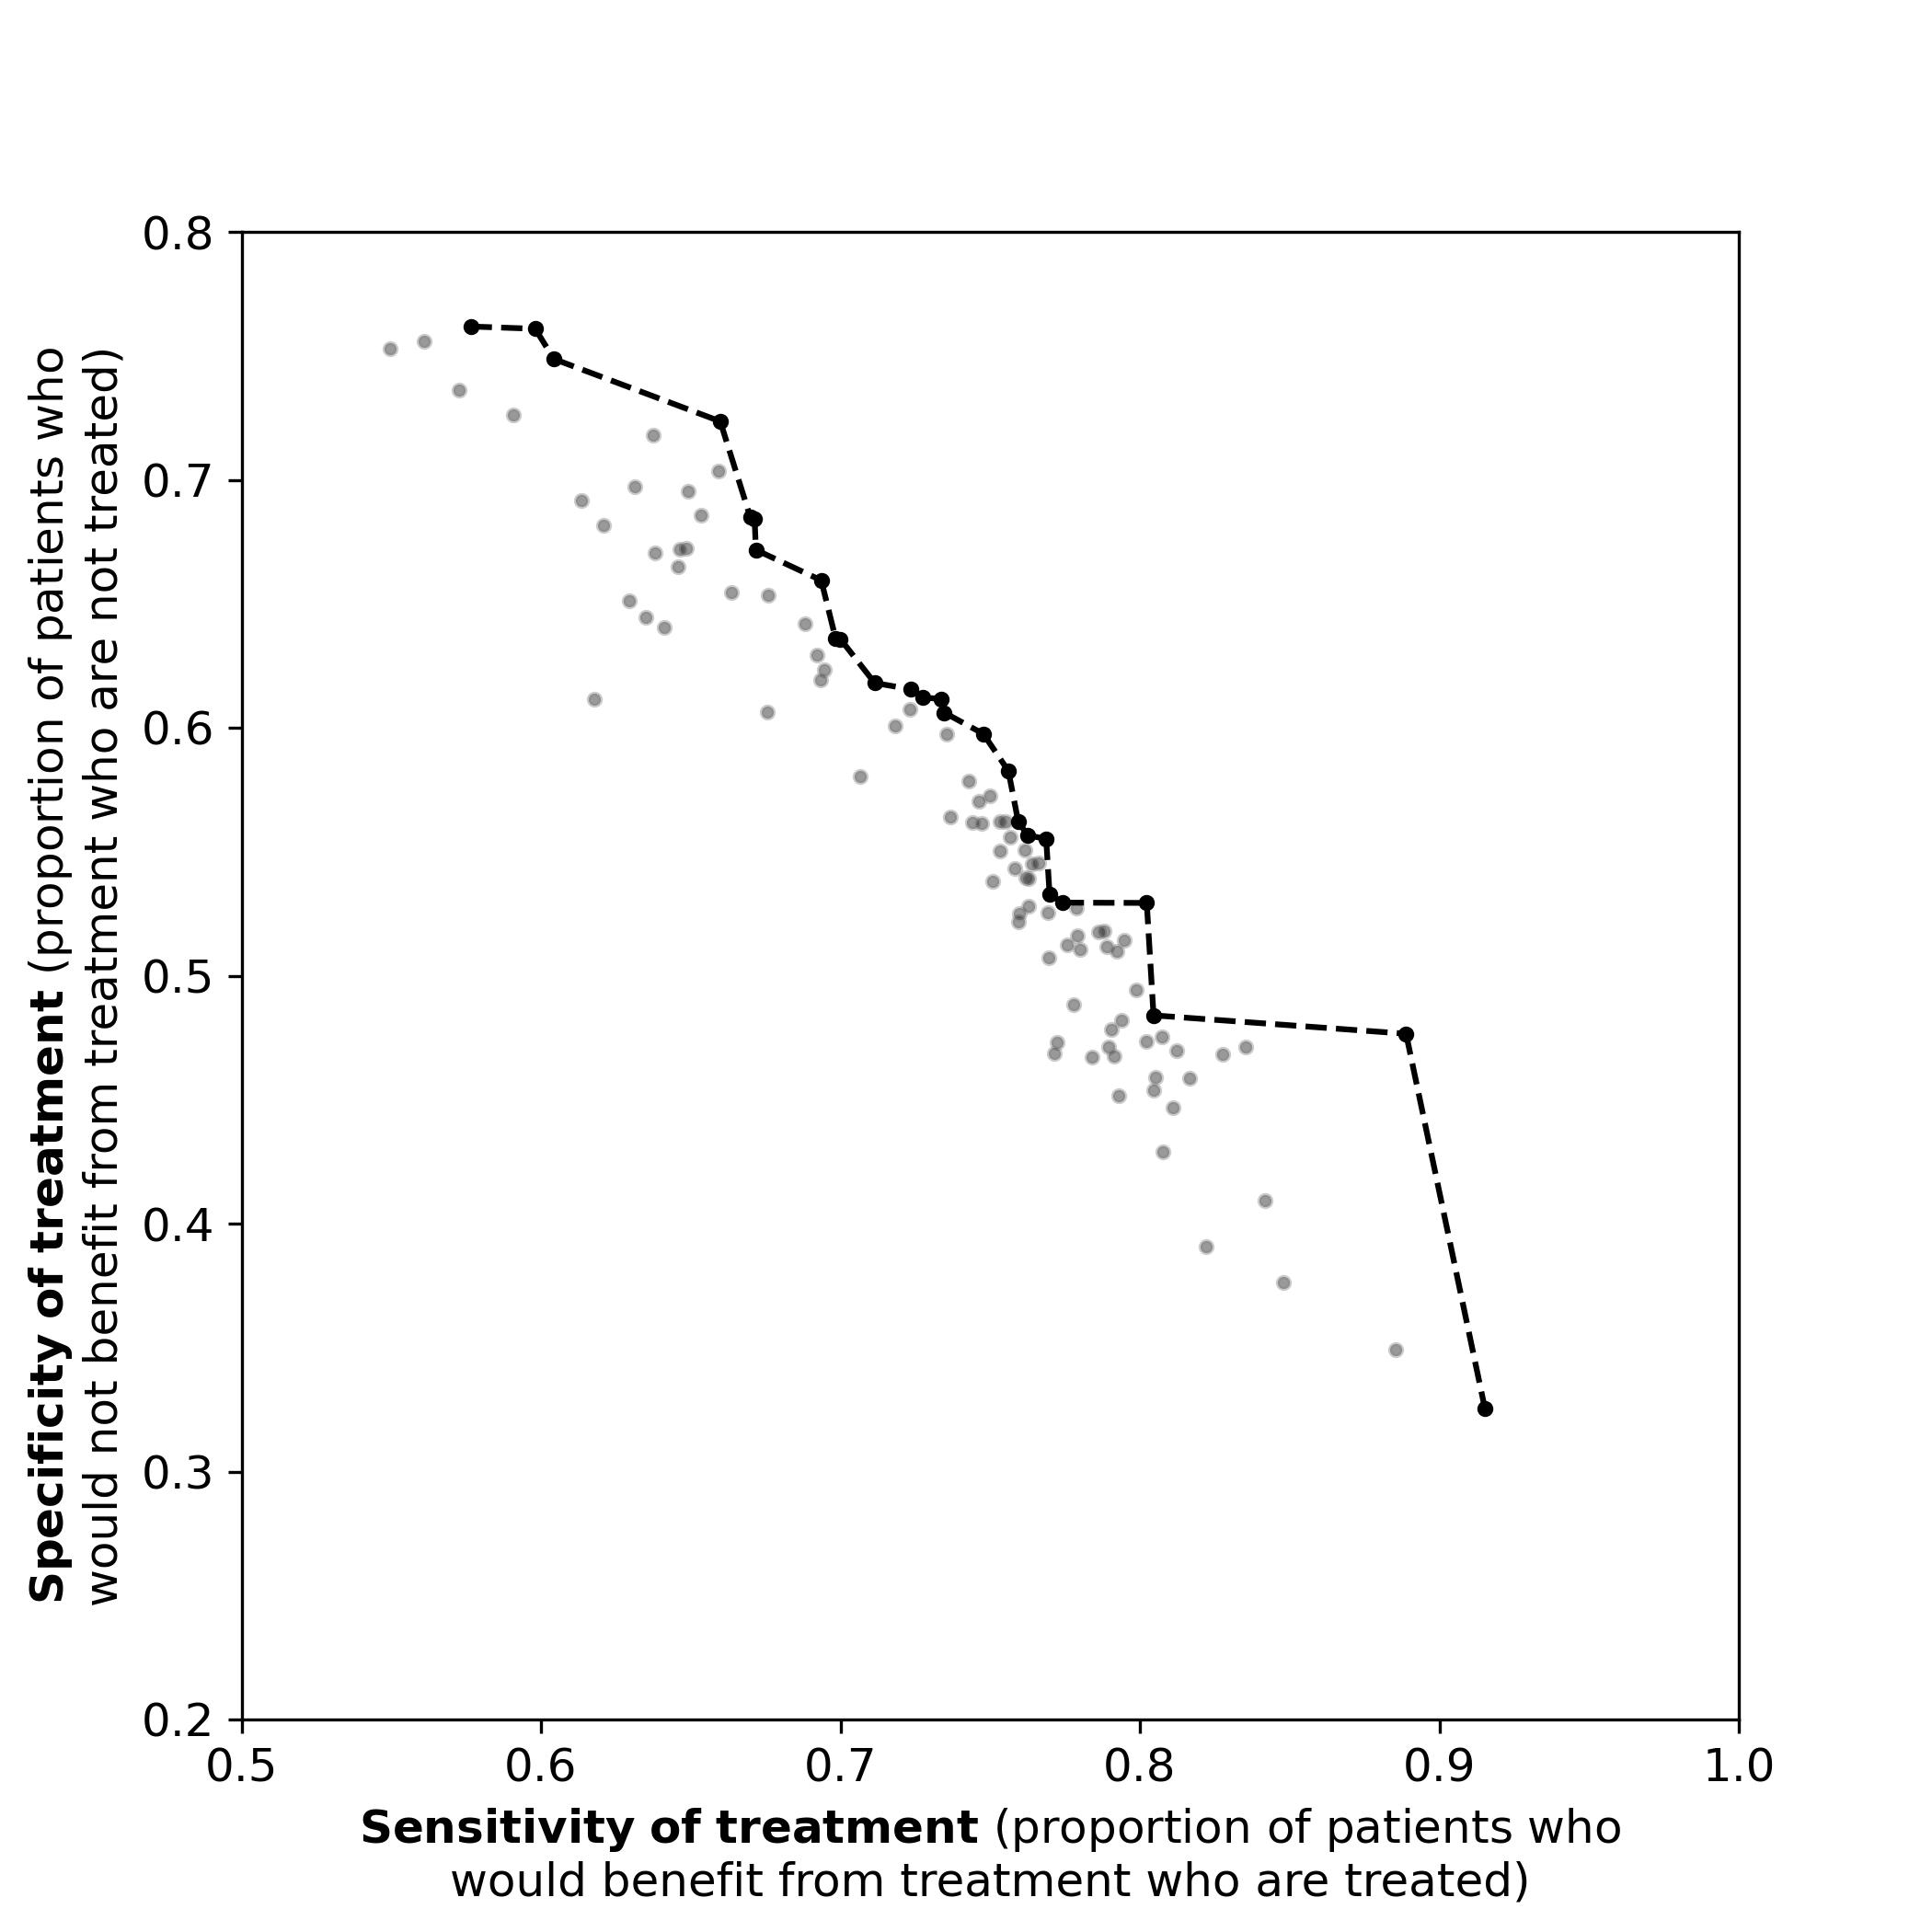
\includegraphics[width=0.65\linewidth]{./images/p4_spec_sens}} 
    \caption{\textit{Sensitivity} (proportion of patients who were predicted to benefit from thrombolysis who were predicted to receive thrombolysis) and \textit{specificity} (proportion of patients who were predicted \textit{not} to benefit from thrombolysis who were predicted \textit{not} to receive thrombolysis) for each stroke team. The dotted line shows the hospitals on the Pareto front where there are no hospitals that have a better \textit{sensitivity} without a worse \textit{specificity}, or vice-versa.}
    \label{fig:hosp_shap_scatter}
\end{figure}


\subsection{Conclusions}

Using machine learning with SHAP in a very large national stroke registry dataset, we found general agreement between actual thrombolysis use and best predicted outcomes, though we found decisions based on the outcome model would support higher use of thrombolysis than is actually the case. Of those who did not receive thrombolysis, the outcome model predicted that nearly half of them would have likely benefited from thrombolysis. Of those that did receive thrombolysis we found about one in four may be being given thrombolysis without there being predicted benefit. There was an apparent trade-off in decision-making between hospitals. Those hospitals who gave thrombolysis to more patients who would benefit from it (higher \textit{sensitivity}) were also more likely to give thrombolysis to more patients who would not benefit from it (lower \textit{specificity}). This represents a trade-off between `\textit{Miss no benefit}' and `\textit{Do no harm}'. Maximising benefit while minimising harm is likely to require more sophisticated guidance on use of thrombolysis, such as that indicated by our model.
\section{Paper 5 highlights: Identifying levers for improving thrombolysis use and outcomes – combining clinical pathway simulation and machine learning applied to the UK stroke registry.\cite{pearn_identifying_2024}} \label{sec:paper_5}

\subsection{Objective}

By combining clinical pathway simulation and machine learning of thrombolysis decision-making and outcomes, we sought to better understand the source of variation in thrombolysis use and the effect on outcomes. We also sought to investigate the cost-effectiveness of thrombolysis in stroke teams with lower or higher thrombolysis use.

\subsection{Methods overview}

\subsubsection{Models}

This work combined four models:

\begin{enumerate}

    \item \textit{Thrombolysis decision model}: An XGBoost machine learning model \cite{chen_xgboost_2016} was used to learn which patients would receive thrombolysis at each stroke team. Stroke team SHAP values were used to identify 25 \textit{benchmark teams} most likely to use thrombolysis. For each patient a \textit{benchmark decision} was predicted, which was the majority vote of the expected decision for that patient at the 25 \textit{benchmark teams}.

    \item \textit{Outcome model}: A XGBoost machine learning model was used to predict outcome (mRS probability distribution) for each patient.

    \item \textit{Patient pathway flow}: Monte-Carlo simulation was used to model the flow of patients through the emergency stroke pathway at each hospital, taking into account both average speeds and variation. When examining the effect of improving patient flow, clinical outcome is predicted as the number of \textit{excellent outcomes} (mRS 0-1) per 1,000 admissions using a previously described mathematical model \cite{allen_estimation_2020}.

    \item \textit{Lifetime economic model}: A model predicting life expectancy, quality-adjusted life years (QALYs), and NHS care costs after stroke, based on age, sex, and disability at discharge\cite{mcmeekin_lifetime_2024}.
    
\end{enumerate}

\subsubsection{Prototype patients}

To help compare decision-making and outcomes across stroke teams we exemplified differences using \textit{prototype patients}. These prototype patients captured a range of features known to affect decisions to treat, and to affect outcomes, and included an \textit{ideal} candidate for thrombolysis. The prototype patients used were:

\begin{enumerate}
    \item \textit{Ideal}: Onset-to-arrival = 90 minutes; arrival-to-scan = 15 minutes; onset-to-thrombolysis = 120 minutes; stroke severity (NIHSS) = 15; pre-stroke disability (mRS) = 0; age = 72.5; precisely known onset; onset not during sleep; stroke type = infarction; patient has no atrial fibrillation and is not receiving anticoagulants for atrial fibrillation.

    \item \textit{Late arrival}: As \textit{ideal} but onset-to-arrival = 225 minutes and onset-to-thrombolysis (when given) = 255 minutes.

    \item \textit{Mild}: As \textit{ideal} but stroke severity = 3.

    \item \textit{Prior disability}: As \textit{ideal} but pre-stroke disability = 3

    \item \textit{Imprecise}: As \textit{ideal} but stroke onset time estimated.

    \item \textit{Age}: As \textit{ideal} but age = 87.5.

    \item Combinations of the above.
\end{enumerate}


\subsubsection{Pathway changes}

The combined model may be used to examine a range of possible changes to improve use of thrombolysis:

\begin{enumerate}

    \item \textit{Base}: Uses the hospitals’ recorded pathway statistics.

    \item \textit{Speed}: Sets 95\% of patients having a scan within 4 hours of arrival, and all patients have 15 minutes arrival-to-scan time and 15 minutes scan-to-needle time.

    \item \textit{Ambo}: Subtracts 15 minutes from the current ambulance-call to arrival-at-hospital times.

    \item  \textit{Onset-known}: Sets the proportion of patients with a known stroke onset time to the national upper quartile if currently less than the national upper quartile.

    \item \textit{Benchmark}: The benchmark thrombolysis rate takes the likelihood to give thrombolysis for patients scanned within 4 hours of onset from the majority vote of the 25 benchmark hospitals (see above).

    \item Combinations of the above.

\end{enumerate}

Code, with demonstration, is available at \url{https://github.com/samuel-book/samuel_2_demo}.


\subsection{Key results}

\subsection{Model accuracy}

Using an 4:1 train:test split, the thrombolysis decision model had an accuracy of 85\%, a balanced accuracy of 82\% (accuracy and balanced accuracy using a 50\% probability cut-off to classify a patient as a binary `likely to receive thrombolysis' or not), and a receiver operating characteristic area under curve of 0.92. The stroke outcome model had a receiver operating characteristic area under curve of 0.80.

\subsection{Benchmark stroke teams and benchmark decisions}

\textit{Benchmark decisions} are those that would likely be taken by the majority 25 \textit{benchmark} stroke teams most likely to use thrombolysis (if all stroke teams saw the same patients). If all decisions-to-treat were made according to benchmark decisions, the average thrombolysis rate across stroke teams would increase from 36\% to 45\% (in the modelled patient population). Thrombolysis use in the 25 stroke teams least likely to use thrombolysis would increase from 29\% to 46\%.

Figure \ref{fig:thrombolysis_rates_teams} compares observed and predicted thrombolysis use (based on historic performance, and applying \textit{benchmark decisions}). Predicted and observed thrombolysis use correlate very closely (r-squared 0.94). Predicted rates were, on average, slightly higher (1.7\%) than observed rates.

\begin{figure}[!h]
    \centering
    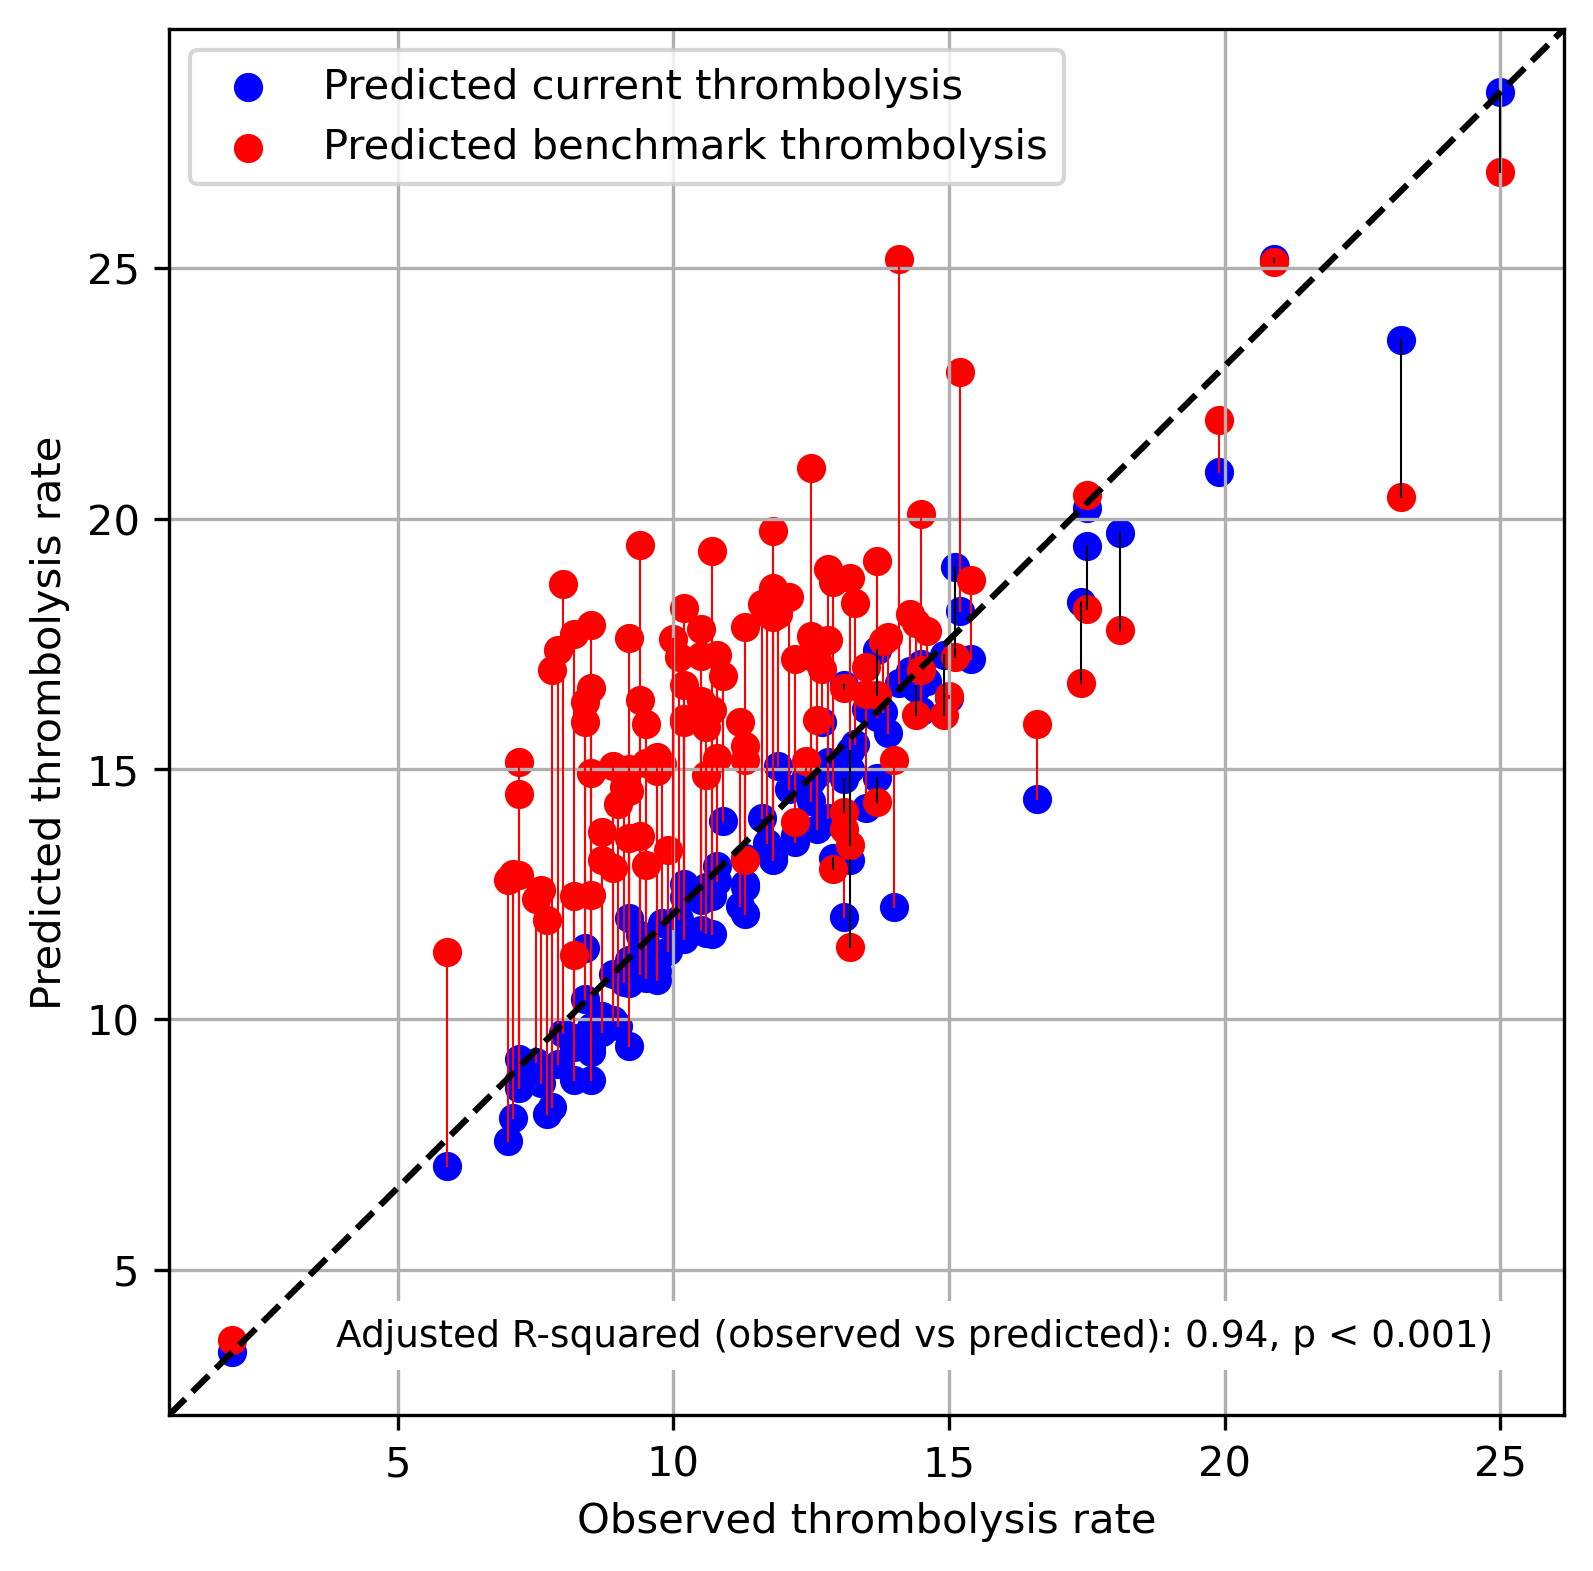
\includegraphics[width=0.5\linewidth]{images/p5_benchmark_rates.png}
    \caption{Comparison of observed and predicted thrombolysis use across stroke teams. Blue circles show predictions based on historic hospital performance. Red circles show the expected thrombolysis use if \textit{benchmark decisions} were made. The black dotted line shows least-squares regression analysis between observed and predicted (using historic performance) thrombolysis use.}
    \label{fig:thrombolysis_rates_teams}
\end{figure}

\subsubsection{Prototype patients}

Prototype patients revealed variation in likely decisions between stroke teams (figure \ref{fig:thrombolysis_rates_prototype_patients}). While almost all stroke teams would give thrombolysis to the \textit{ideal} candidate for thrombolysis, the predicted use of thrombolysis varied more as one characteristic was changed from the \textit{ideal} candidate. In particular there was a very wide range in likelihood of a patient with a mild stroke (NIHSS 3) receiving thrombolysis. Mild stroke (NIHSS 0-4) represents a large proportion of admissions (54\% of all emergency stroke admissions, and 38\% of ischaemic stroke patients arriving by ambulance within 4 hours of known stroke onset). Combinations of \textit{non-ideal} patient characteristics reduced predicted use of thrombolysis further (again with significant variation between stroke teams), especially when the non-ideal characteristic was a mild stroke.

\begin{figure}
    \centering
    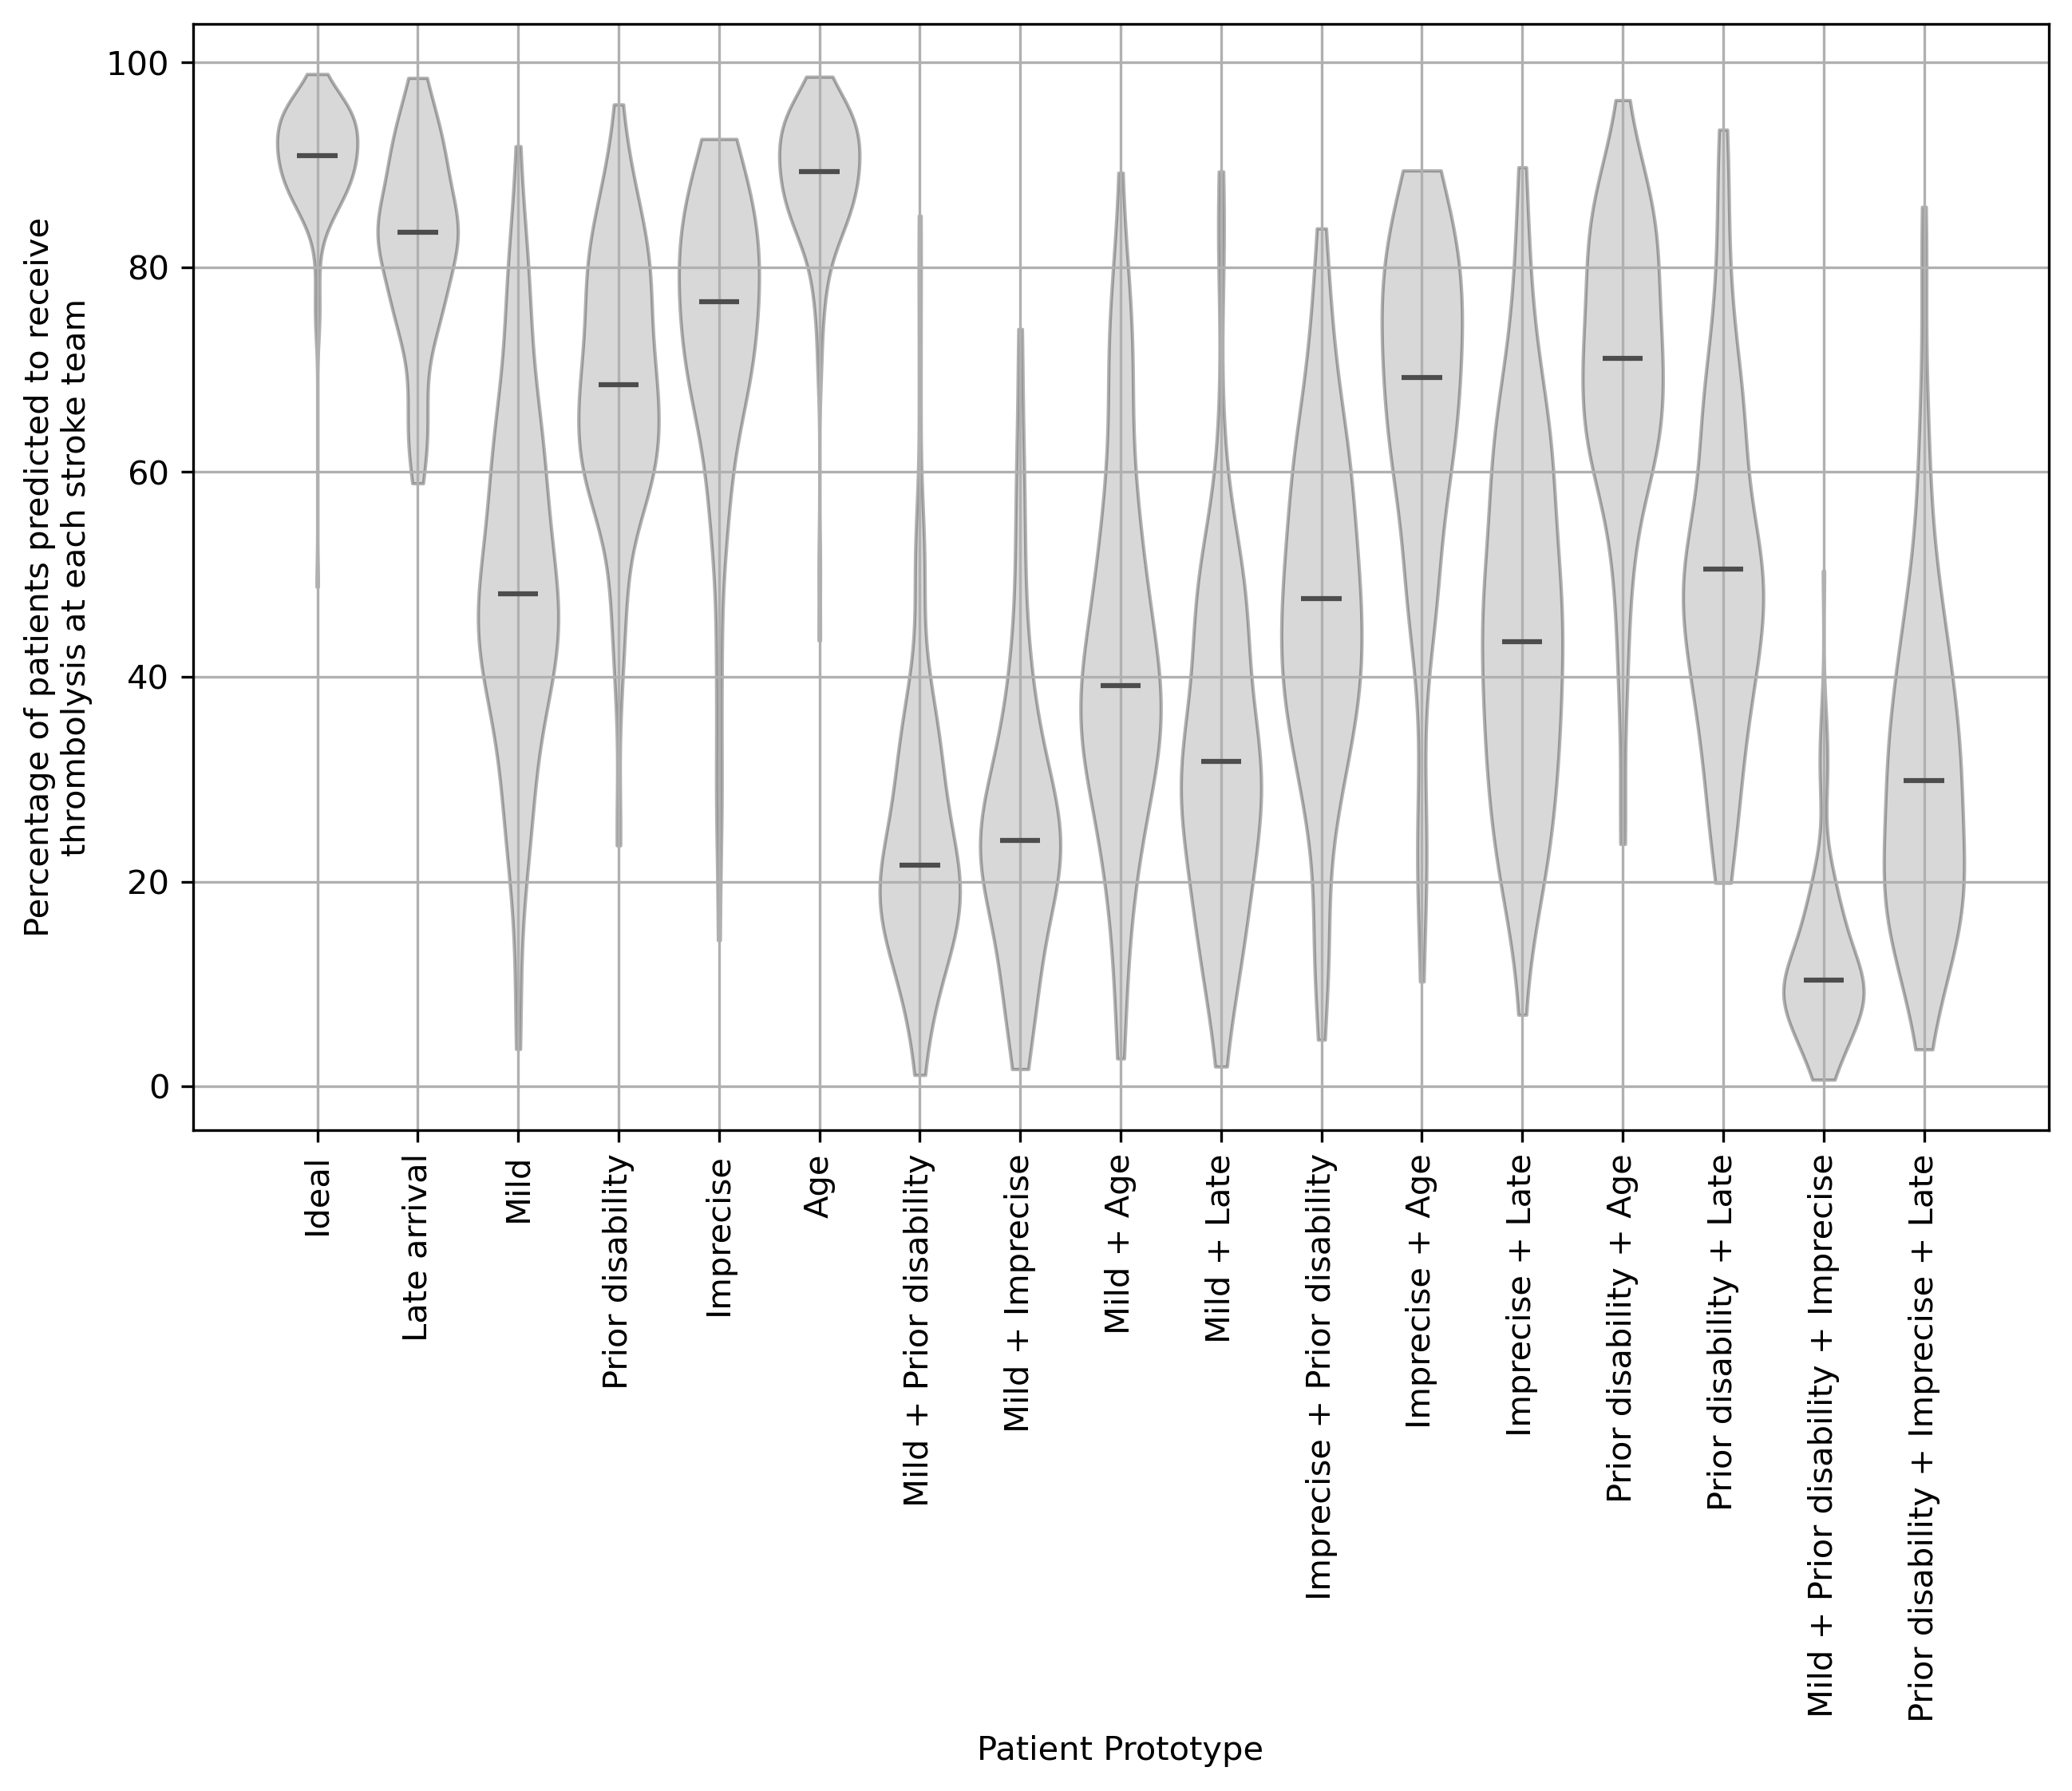
\includegraphics[width=0.75\linewidth]{images/p5_prototype_decision.png}
    \caption{Violin plots showing the variation in predicted thrombolysis rates for 17 patient prototypes across stroke teams. \textit{Ideal}: onset-to-arrival = 90 minutes; arrival-to-scan = 15 minutes; onset-to-thrombolysis = 120 minutes; stroke severity (NIHSS) = 15; pre-stroke disability (mRS) = 0; age = 72.5; precisely known onset; onset not during sleep; stroke type = infarction; patient has no atrial fibrillation and is not receiving anticoagulants for atrial fibrillation; \textit{Late arrival}: as \textit{ideal} but onset-to-arrival = 225 minutes and onset-to-thrombolysis = 255 minutes; \textit{Mild}: As \textit{ideal} but stroke severity = 3; \textit{Prior disability}: as \textit{ideal} but pre-stroke disability = 3; \textit{Imprecise}: as \textit{ideal} but stroke onset time estimated; \textit{Age}: as \textit{ideal} but age = 87.5.}
    \label{fig:thrombolysis_rates_prototype_patients}
\end{figure}

Table \ref{tab:prototype_outcomes} shows predicted outcomes across all prototype patients. All these patients would likely benefit from thrombolysis, but the benefit in mild stroke was smaller.

\begin{minipage}{1\textwidth}
\small
\begin{longtable}{p{5.2cm} | p{1.6cm} p{1.6cm} p{1.5cm} | p{1.6cm} p{1.6cm} p{1.5cm}}
\caption{Predicted outcomes for patient prototypes. \textit{Ideal}: onset-to-arrival = 90 minutes; arrival-to-scan = 15 minutes; onset-to-thrombolysis = 120 minutes; stroke severity (NIHSS) = 15; pre-stroke disability (mRS) = 0; age = 72.5; precisely known onset; onset not during sleep; stroke type = infarction; patient has no atrial fibrillation and is not receiving anticoagulants for atrial fibrillation. \textit{Late arrival}: as \textit{Ideal} but onset-to-arrival = 225 minutes and onset-to-thrombolysis = 255 minutes; \textit{Mild}: as \textit{Ideal} but stroke severity = 3; \textit{Prior disability}: as \textit{Ideal} but pre-stroke disability = 3; \textit{Imprecise}: as \textit{ideal} but stroke onset time estimated. \textit{Age}: as \textit{Ideal} but age = 87.5. Results also includes patients prototypes with combinations of these non-ideal characteristics. Results show probability-weighted disability at discharge, and the proportion of patients predicted to have a very poor outcome (mRS 5-6).}\\
\label{tab:prototype_outcomes}
Patient prototype & Untreated probability-weighted mRS & Treated probability-weighted mRS & Improve-ment & Untreated proportion mRS 5-6 & Treated proportion mRS 5-6 & Improve-ment\\
\endhead
\midrule
Ideal & 3.39 & 2.37 & 1.02 & 0.32 & 0.13 & 0.19\\
Late & 3.39 & 2.73 & 0.66 & 0.32 & 0.18 & 0.14\\
Mild & 1.15 & 0.91 & 0.23 & 0.01 & 0.01 & 0.00\\
Prior disability & 4.22 & 3.61 & 0.61 & 0.41 & 0.23 & 0.19\\
Imprecise & 3.49 & 2.39 & 1.10 & 0.33 & 0.13 & 0.20\\
Age & 4.22 & 3.51 & 0.71 & 0.50 & 0.35 & 0.16\\
Mild + Prior disability & 2.92 & 2.60 & 0.32 & 0.04 & 0.04 & 0.00\\
Mild + Imprecise & 1.28 & 1.01 & 0.26 & 0.02 & 0.01 & 0.00\\
Mild + Age & 1.84 & 1.63 & 0.22 & 0.04 & 0.03 & 0.01\\
Mild + Late & 1.15 & 0.77 & 0.39 & 0.01 & 0.00 & 0.00\\
Imprecise + Prior disability & 4.33 & 3.67 & 0.66 & 0.44 & 0.24 & 0.20\\
Imprecise + Age & 4.31 & 3.57 & 0.74 & 0.53 & 0.36 & 0.17\\
Imprecise + Late & 3.49 & 2.75 & 0.74 & 0.33 & 0.17 & 0.17\\
Prior disability + Age & 4.62 & 4.35 & 0.27 & 0.53 & 0.44 & 0.08\\
Prior disability + Late & 4.22 & 3.70 & 0.52 & 0.41 & 0.27 & 0.14\\
Mild + Prior disability + Imprecise & 3.01 & 2.65 & 0.36 & 0.06 & 0.06 & 0.00\\
\end{longtable}
\normalsize
\end{minipage}

\subsubsection{Pathway improvement}

Across the study population, by combining pathway improvements, thrombolysis use in all those emergency stroke admissions arriving by ambulance shows the potential to be increased from 13\% to 20\% (figure \ref{fig:scenarios_population}). Using a model based on clinical trial data, benefit, as measured by number of number of people discharged with no, or minimal, disability (mRS 0 or 1) could be doubled from 10 to 20 additional excellent outcomes per 1,000 admissions. The single most influential change in improving thrombolysis use was applying \textit{benchmark} decisions (figure \ref{fig:scenarios_population}, left panel). Improving speed would not greatly increase the number of people given thrombolysis, but would lead to more benefit from thrombolysis as all treated patients will gain benefit from earlier treatment (figure \ref{fig:scenarios_population}, left panel).

\begin{figure}
    \centering
    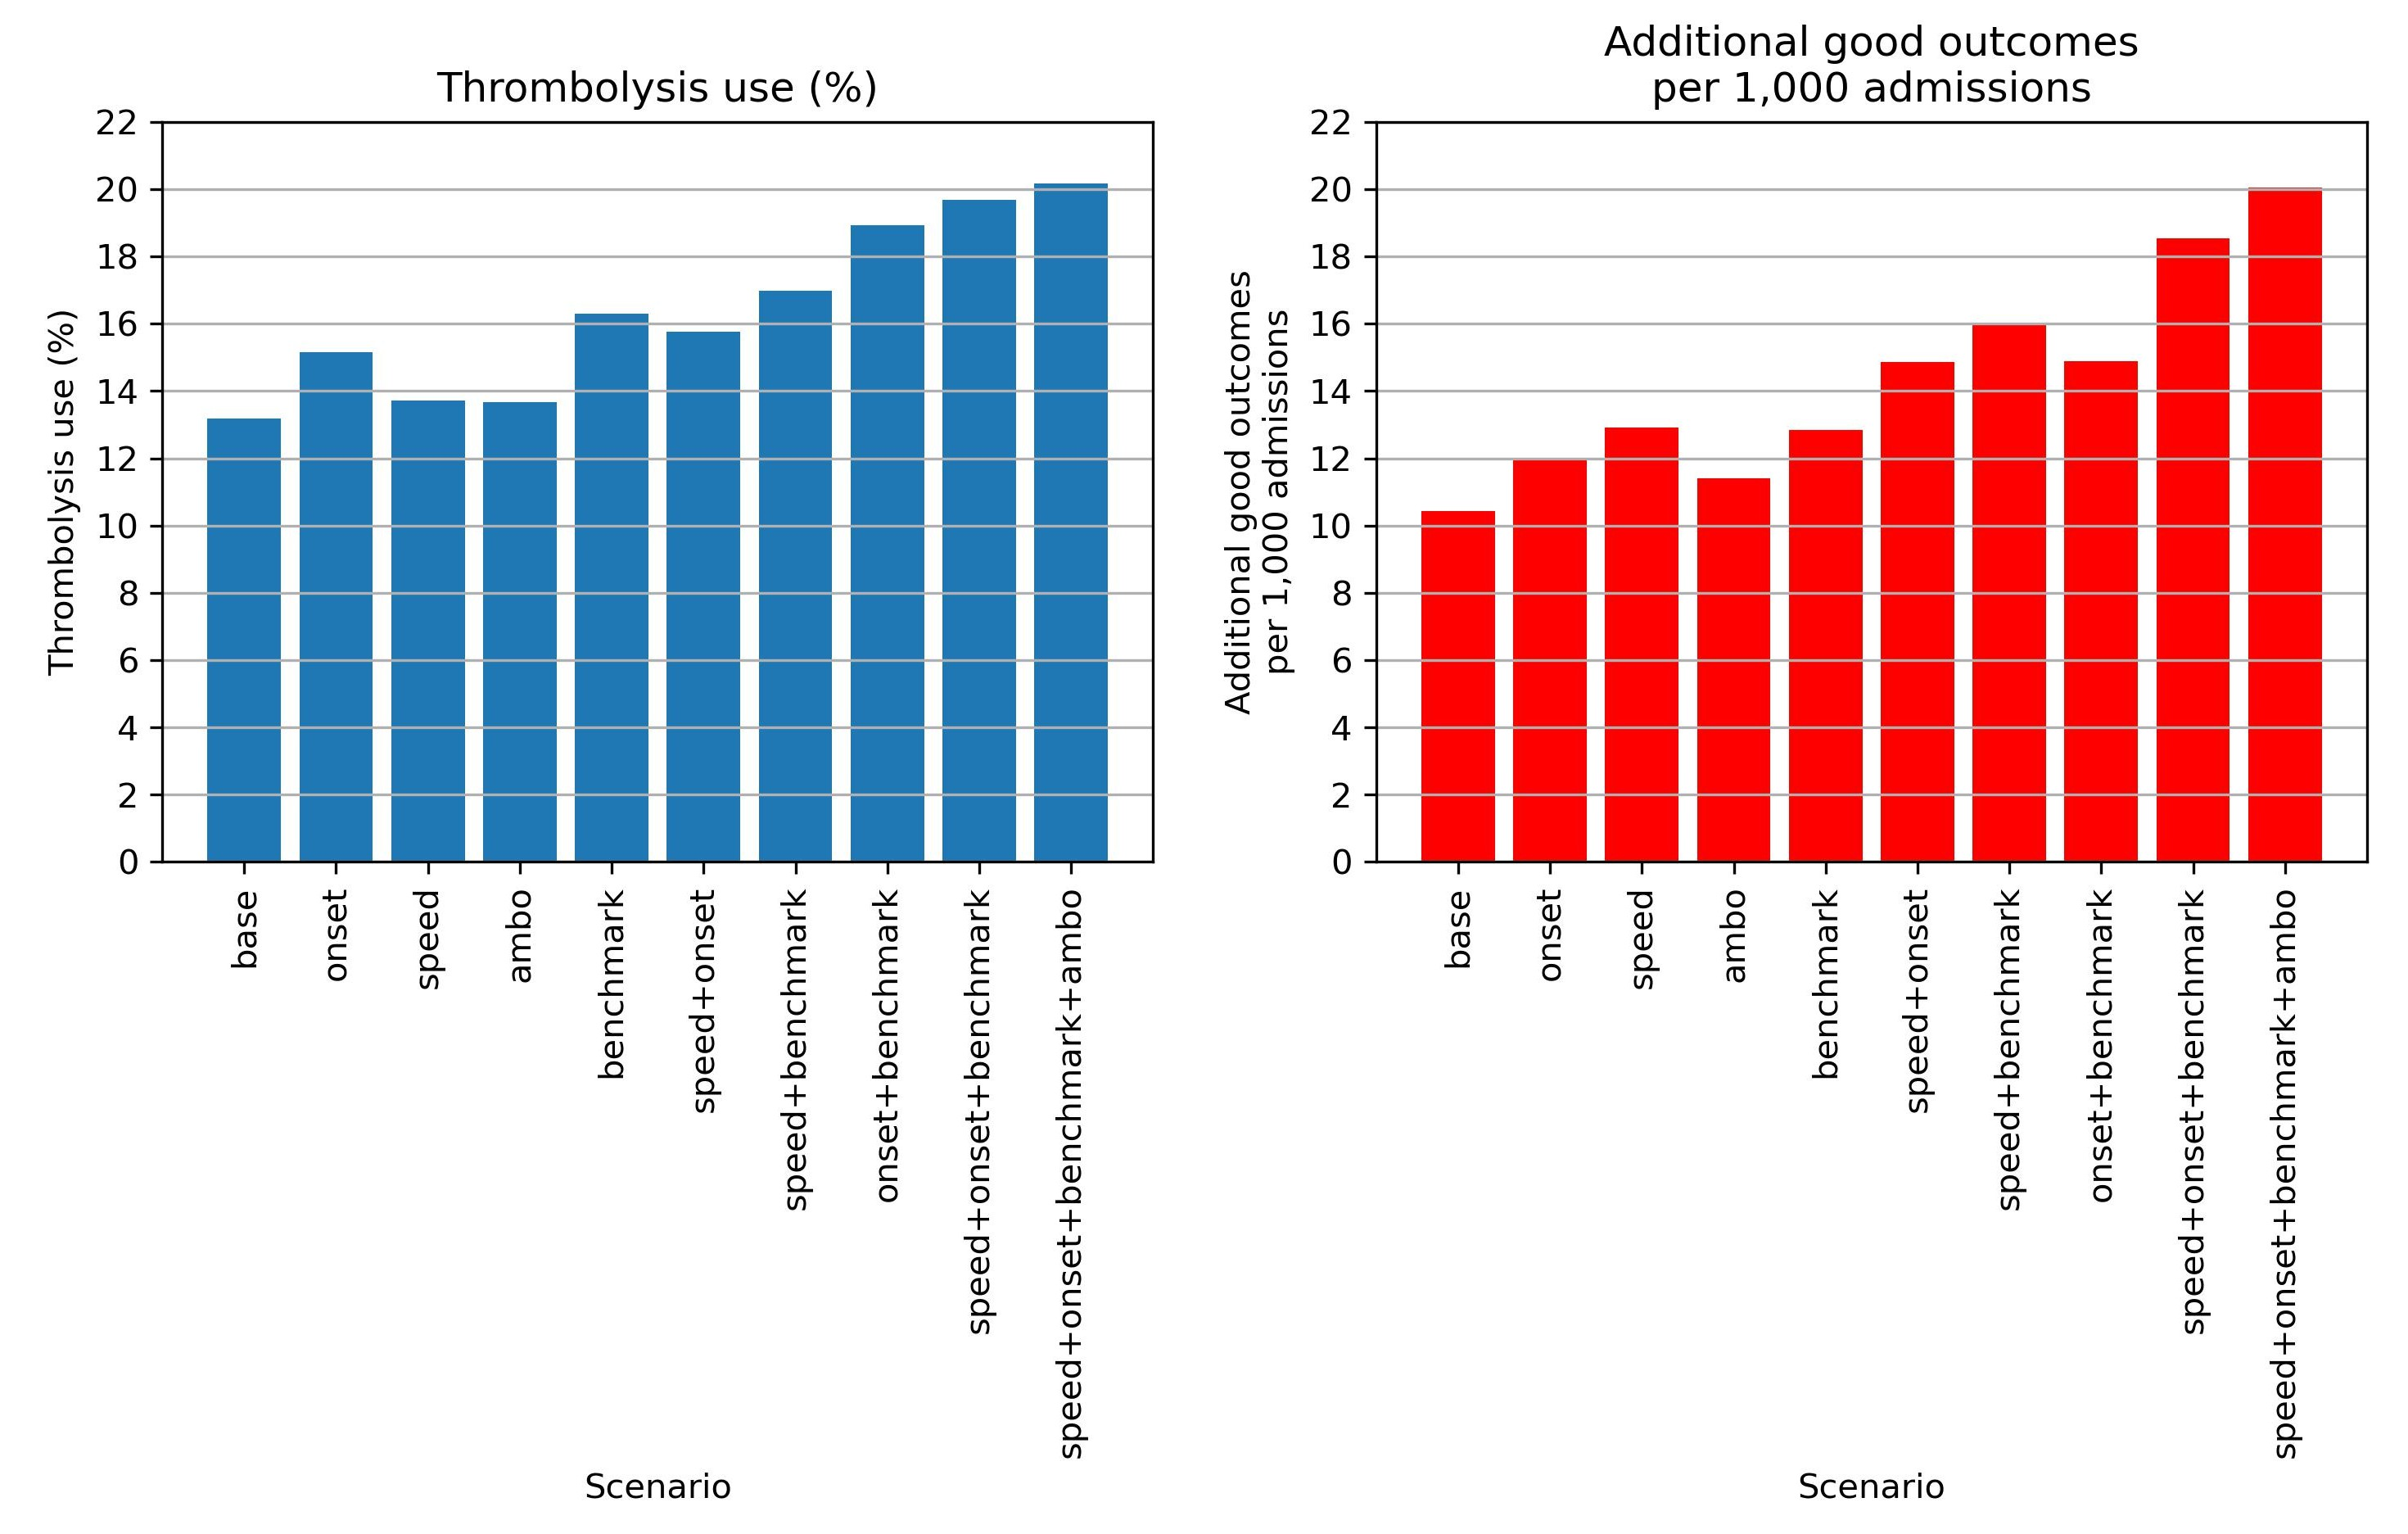
\includegraphics[width=1\linewidth]{images/p5_sim.jpg}
    \caption{Expected effect of alternative process improvement initiatives across the study population. The chart shows the effect on thrombolysis use (left) and on number of additional excellent outcomes (mRS 0-1) per 1,000 admissions due to use of thrombolysis (right). \textit{Base}: Uses the hospitals’ recorded pathway statistics. \textit{Onset}: Sets the proportion of patients with a known stroke onset time to the national upper quartile if currently less than the national upper quartile. \textit{Speed}: Sets 95\% of patients having a scan within 4 hours of arrival, and all patients have 15 minutes arrival-to-scan time and 15 minutes scan-to-needle time. \textit{Ambo}: Subtracts 15 minutes from the current ambulance call to arrival-at-hospital times. \textit{Benchmark}: The benchmark thrombolysis rate takes the likelihood to give thrombolysis for patients scanned within 4 hours of onset from the majority vote of the 25 benchmark hospitals.}
    \label{fig:scenarios_population}
\end{figure}

\FloatBarrier

\subsection{Lifetime economic model}

Table \ref{tab:health_econ} shows the modelled health economics of thrombolysis use, comparing actual use of thrombolysis with \textit{benchmark} thrombolysis use. The effect of thrombolysis was estimated by predicting the outcomes with and without thrombolysis for the two groups (those that actually received thrombolysis, and those predicted to receive thrombolysis using \textit{benchmark} decisions). Benchmark decisions maintain the benefit of using thrombolysis, but extend that benefit to more patients. This extended benefit was not at the cost of any predicted increase in the worst outcomes (mRS 5-6). The extended benefit led to more QALYs added across the population by treatment, and more predicted savings to NHS healthcare costs.

\begin{table}[!h]
\small
\caption{Health economic analysis: Analysis for  populations based on predicted benefit (or dis-benefit) of thrombolysis. The effect of thrombolysis was estimated by predicting the outcomes with and without thrombolysis for the two groups (those that actually received thrombolysis, and those predicted to receive thrombolysis using \textit{benchmark} decisions). The analysis compares the populations currently treated, or the population that would be treated using \textit{benchmark} decisions (the majority vote of the predicted choice of the the 25 stroke teams most likely to use thrombolysis). Results are shown for (a) the treated populations, and (b) adjusted for 1,000 emergency stroke admissions }
\label{tab:main}

\begin{subtable}{1\textwidth}
\centering
\caption{Counterfactual analysis of the effect of thrombolysis in either those patients who actually received thrombolysis, or those patients where the \textit{benchmark decision} would be to use thrombolysis.}
\begin{tabular}{p{2.0cm} p{1.5cm} p{1.2cm} p{1.3cm} p{1.5cm} p{1.3cm} p{1.4cm} p{1.3cm} p{1.3cm}}
\toprule
Population & \raggedright Modelled treatment & Death & Survival (median years) & Care years (median) & QALYs & \raggedright Discounted cost per patient & Proportion mRS 0-2 & Proportion mRS 5-6\tabularnewline
\midrule
Actual use & Untreated & 17.1\% & 7.60 & 0.28 & 5.020 & £20,370 & 47.1\% & 23.9\%\tabularnewline
& Treated & 14.2\% & 7.91 & 0.25 & 5.258 & £19,806 & 53.9\% & 19.3\%\tabularnewline
& Difference & -2.9\% & 0.31 & -0.03 & 0.238 & -£565 & 6.8\% & -4.7\%\tabularnewline
\midrule
Benchmark & Untreated & 17.4\% & 7.63 & 0.28 & 5.036 & £20,388 & 46.5\% & 24.1\%\tabularnewline
& Treated & 14.4\% & 7.93 & 0.25 & 5.269 & £19,784 & 53.4\% & 19.4\%\tabularnewline
& Difference & -3.0\% & 0.30 & -0.03 & 0.234 & -£603 & 6.9\% & -4.8\%\tabularnewline

\end{tabular}
\end{subtable}

\vspace{3mm}

\begin{subtable}{1\textwidth}
\centering
\caption{Analysis for 1,000 emergency stroke admissions (all stroke types)}
\begin{tabular}{p{1.9cm} p{1.9cm} p{1.9cm} p{1.9cm} p{1.9cm} p{1.9cm} p{2.2cm}}
\toprule
Population & Proportion treated & QALYs added & Healthcare costs saved & \raggedright Thrombolysis cost (£450 per patient) & \raggedright Cost per QALY added & \raggedright Net cost of thrombolysis\tabularnewline
\midrule
Actual & 11.0\% & 26.3 & £62,294 & £49,658 & £1,890 & -£12,637\tabularnewline
Benchmark & 13.6\% & 31.7 & £81,914 & £61,117 & £1,927 & -£20,797\tabularnewline
\bottomrule
\end{tabular}
\end{subtable}
\label{tab:health_econ}
\end{table}

\normalsize

\FloatBarrier

\subsection{Conclusions}

There is significant inter-hospital variation in use of thrombolysis that is caused by hospital processes and differences in decision-making. Improving processes and adopting the decision making of higher-thrombolysing units would be expected to increase thrombolysis use and has the potential to double the population benefit from thrombolysis. Higher-thrombolysing sites are delivering greater cost-effectiveness from thrombolysis through reductions in long-term disability in a greater number of patients.  Pathway analysis and machine learning should allow stroke teams to better understand, and improve, their own pathways.
\section{Other project outputs}

\subsection{Predicting willingness to use thrombolysis from SSNAP organisational audit data}

We performed a model to investigate whether organisational audit results reported by SSNAP could be used to predict a teams. The SSNAP Organisational Audit collects biennial data on the structure and organization of acute hospital stroke services, including bed numbers, staffing and seniority levels (including at the ‘front door’), models of delivery of hyperacute services including reperfusion, and other structural data. We devised a model to investigate whether organisational audit data reported by SSNAP could be used to predict a team’s propensity to use thrombolysis, as measured by the SHAP value for the stroke team in the thrombolysis decision model. We were not able to identify any significant predictors of ‘willingness to thrombolyse’ from these data, indicating that there were no features of the organisation of hyperacute staffing or other provision, including unit size and admission numbers, that were predictive of a site’s propensity to use thrombolysis (see \url{https://github.com/samuel-book/thrombolysis_organisational_factors/blob/main/data_prep/2c_statsmodels.ipynb}). This finding runs counter to the often-cited notion that sites with higher rates of thrombolysis tend to be those that are larger and better staffed. Evidence is clear that organisation factors do affect thrombolysis use \cite{carter-jones_stroke_2011}; we simply did not find a strong link between willingness to use thrombolysis and the organisational audit output. This could be due to the SSNAP Organisational Audit recording numbers from a single day snap shot, and more frequent data collection may enable identification of significant predictors of ‘willingness to thrombolyse’.

\subsection{Pilot thrombectomy model}

As part of this study we performed a pilot experiment on the effect of thrombectomy (mechanical removal of the clot) on outcomes in severe stroke (NIHSS 11+). The same model method was used as the outcome modelling with thrombolysis, but time from onset to thrombectomy was also added. Figure \ref{fig:thrombectomy} shows the relationship between time from onset to thrombectomy. \textbf{These results have not been robustly investigated, and should be taken as indicative only}, but we saw a beneficial effect of thrombectomy. The effect of thrombectomy decayed over time. Early thrombectomy was able to significantly improve the odds of being discharged (with this effect being in addition to the effect of thrombolysis). More work is required to confirm and better understand this effect, with the significantly larger number of patients who have received thrombectomy that is now in SSNAP.

\begin{figure}[!h]
    \centering
    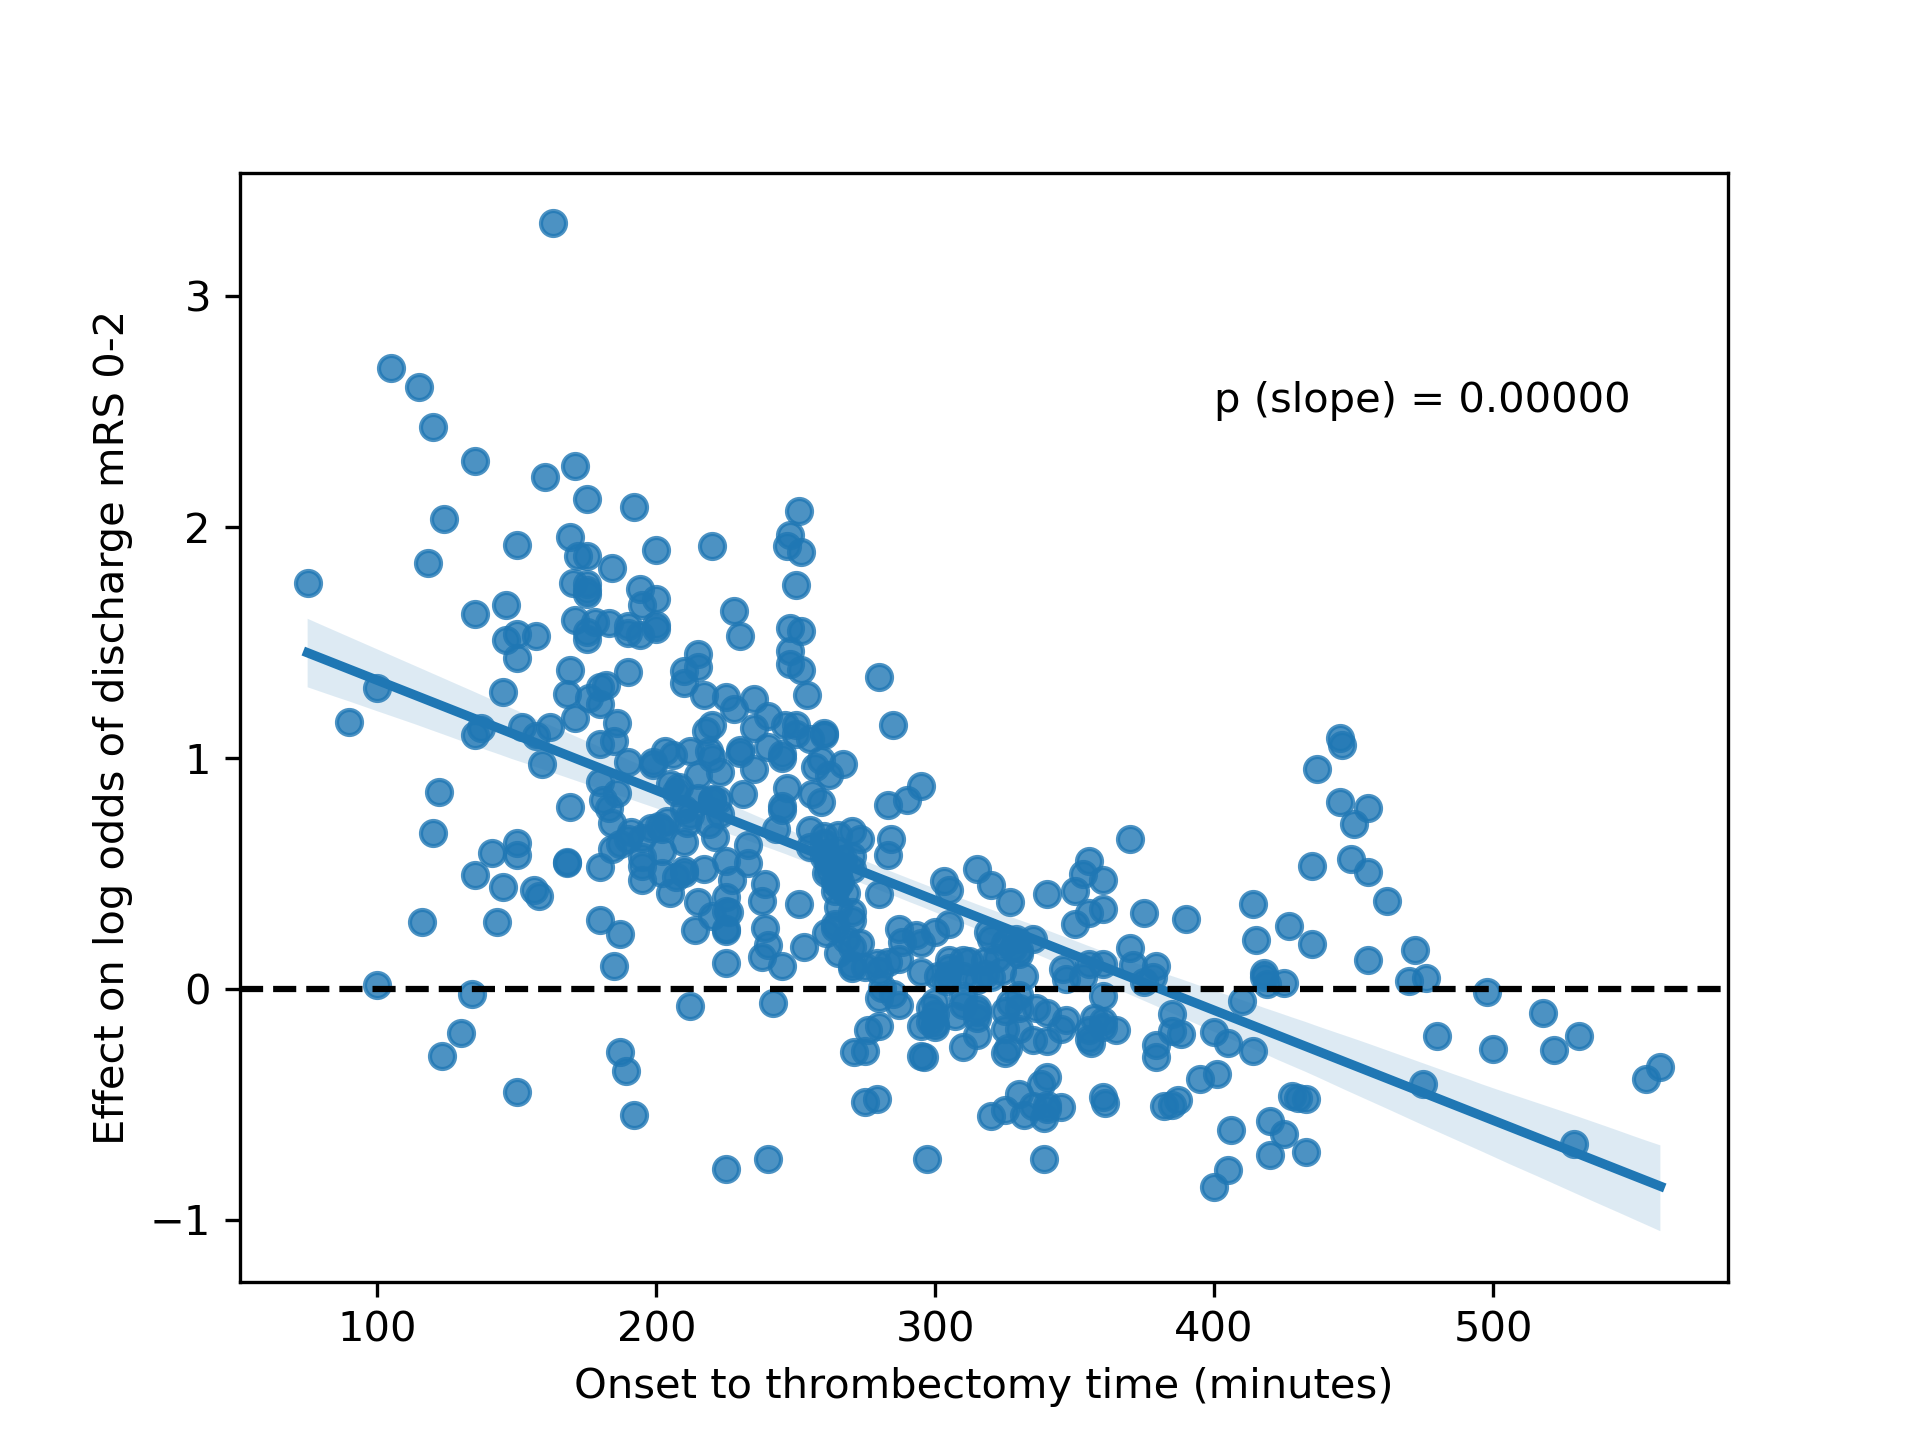
\includegraphics[width=0.75\linewidth]{images/thrombectomy}
    \caption{The effect of time of onset to thrombectomy on the log of odds of being discharged with mRS 0-2 for patients with stroke severity of NIHSS 11+ (using the SHAP value for the effect of thrombectomy). Data shown is for 411 patients that received thrombectomy within 10 hours of stroke onset. This effect is the effect of thrombectomy in addition to any effect of thrombolysis. \textbf{Results show pilot work and should be taken as indicative only}.}
    \label{fig:thrombectomy}
\end{figure}




\section{Discussion}

\subsection{Principle findings}

See section{\label{sec:papers}} for an overview of key findings.

Qualitative research identified that:

\begin{itemize}
    \item It is important to demonstrate integrity of the modelling, given some concerns about the quality of individual SSNAP data.

    \item Evidence from this research and elsewhere indicates that the ED physicians’ may have less confidence in the evidence base for, and safety of thrombolysis.

    \item Perceived lack of funding/resource and stroke workforce shortages may impede quality improvement and adoption of new technologies such as SAMueL-2. It will therefore be vital to address these concerns to ensure sustained use and adoption.

\end{itemize}

Machine learning and modelling identified that:

\begin{itemize}
    \item Thrombolysis use in patients arriving within 4 h of known or estimated stroke onset ranged 7\% -49\% between hospitals. 
    
    \item The odds of receiving thrombolysis reduced 9-fold over the first 120 min of arrival-to-scan time, varied 30- fold with stroke severity, reduced 3-fold with estimated rather than precise stroke onset time, fell 6-fold with increasing pre-stroke disability, fell 4-fold with onset during sleep, fell 5-fold with use of anticoagulants, fell 2-fold between 80 and 110 years of age, reduced 3-fold between 120 and 240 min of onset-to-arrival time and varied 13-fold between hospitals. 
    
    \item The majority of between-hospital variance in thrombolysis use, in patients arriving within 4 h of known or estimated stroke onset, was explained by the hospital, rather than the differences in local patient populations.
    
    \item Thrombolysis was found to be associated with a statistically significant improvement in the odds of having a good outcome using any mRS threshold. Regression analysis predicted a maximum 2.5-fold improvement in odds of achieving mRS 0-1, with a decline to no treatment effect at 5 hours 28 minutes post-onset. The observed beneficial effect is very similar to Emberson’s meta-analysis of a maximum 2.0-fold improvement in odds of achieving mRS 0-1, with a decline to no treatment effect at 6 hours 88 minutes post-onset.
    
    \item Of those patients arriving by ambulance, who had a head scan within 225 minutes of known or estimated stroke onset, and were not takinf anticoagulant medication for atrial fibrillation, 60\% were predicted to have a better outcome with thrombolysis (improved probability-weighted mRS and reduced probability of mRS 5-6). 73\% of those treated were predicted to have a better outcome with thrombolysis, and 49\% of those not treated were predicted to have a better outcome with thrombolysis. Patients with mismatched treatment decisions (actual thrombolysis use vs. predicted to benefit) can not be identified from an isolated feature value. Individual hospitals vary in balancing maximising benefit from thrombolysis vs. avoiding any possible harm.
    
    \item Combining potential changes (improving arrival-to-thrombolysis times to 30 mins, reducing ambulance call-to-hospital-arrival times by 15 minutes, having all teams attain the current upper-quartile performance in determining stroke onset time, and applying decision making similar to high thrombolysing units) would be expected to increase thrombolysis use in patients arriving by ambulance from 13\% to 20\% and double the clinical benefit (additional patients discharged mRS 0-1) from thrombolysis.
    
    \item The largest single factor in improving both thrombolysis use and outcomes is differences in clinical decision-making. Stroke teams vary in clinical decision-making especially in subgroups of patients with features that make them non-ideal candidates for thrombolysis: mild stroke, pre-existing disability, and imprecisely known stroke onset times.
    
    \item High thrombolysing units are predicted to be generating more net benefit (including better avoidance of mortality and severe disability) than low thrombolylsing units.
    
    \item A health economics model, using the output from the outcome prediction model, estimated that thrombolysis produces an additional 0.26 QALY for each person treated.
    \end{itemize}

\subsection{Clinical discussion}

% See https://www.journalslibrary.nihr.ac.uk/information-for-authors/journals-library-publication-approaches/Threaded-Publication/synopsis.htm

\section{Patient and Public Involvement}

% Include involvem,ent and plans (YouTube, articles for stroke groups)

\section{Equality, Diversity and Inclusion (EDI)}

Though EDI was not a focus of this particular project's objectives, to build substantial EDI into future work, we have performed the ground work required to link analysis of stroke treatment and outcomes to population demographics for each stroke team. We have combined data from multiple sources (at Lower Super Output Area) and collated according to stroke unit catchment areas (estimated by assigning each LSOA to the stroke team with the shortest travel time), and other areas such as Integrated Stroke Delivery Networks, and ambulance trust.

Data (source data and combined data) and code for this is available at: \url{https://github.com/samuel-book/stroke_unit_demographics}. Analysis is also made available by a web application at: \url{https://stroke-unit-demographics.streamlit.app/Interactive_demo}.

\section{Impact and Learning}

\section{Implications for decision makers}

\section{Research recommendations}

\section{Conclusions}

\section{Acknowledgements}

We would like to thank our Patient and Carer Involvement team led by Leon Farmer (David Burgess, Simon Douglas, Ian Hancock, Nicola Hancock, John Williams), and our expert advisory group (Ajay Bhalla, Gary Ford, Martin Utley).

\section{Declaration of conflicting interests}

The authors declare no potential conflicts of interest with respect to the research, authorship, and/or publication of this article. 

\section{Funding}

The authors disclose receipt of the following financial support for the research, authorship, and/or publication of this article: This research was funded by the National Institute for Health Research Applied Research Collaboration South West Peninsula and by the National Institute for Health Research Health and Social Care Delivery Research (HSDR) Programme [NIHR134326]. The views expressed in this publication are those of the authors and not necessarily those of the National Institute for Health Research or the Department of Health and Social Care. 



\bibliographystyle{naturemag}
%\bibliographystyle{plainnat}
%\bibliographystyle{unsrt}
%\bibliographystyle{unsrtnat}
\bibliography{references}

% Number for supplementary material
\newcommand{\beginsupplement}{
    \setcounter{section}{0}
    \renewcommand{\thesection}{A\arabic{section}}
    \setcounter{figure}{0}
    \renewcommand{\thefigure}{A\arabic{figure}}
    \setcounter{table}{0}
    \renewcommand{\thetable}{A\arabic{table}}
}
\beginsupplement


%TC:igno
\addcontentsline{toc}{section}{APPENDIX}

\section{Descriptive statistics}
\label{sec:stats}

Tables \ref{tab:hospital_stats_1} to \ref{tab:hospital_stats_3} show descriptive statistics for patients (2016-2021) across all stroke teams for (1) all patients, patients arriving within 4 hours of known stroke onset, and patients arriving by ambulance within 4 hours of known stroke onset. These statistics are for 5 years arrivals (2017-2021).

\begin{minipage}{1\textwidth}
\small
\renewcommand{\arraystretch}{1.3}
\begin{longtable}{p{7cm} p{1cm} p{0.8cm} p{0.8cm} p{0.8cm} p{0.8cm} p{0.8cm} p{0.8cm} p{0.8cm} p{0.8cm}}
\caption{Descriptive statistics for all patients (n = ?) arriving at each stroke team. The table shows summary statistics across all stroke teams capturing each feature.}\\
\toprule
\endhead
Statistic & Stroke teams & mean & Std Dev & min & 25\% & 50\% & 75\% & max\tabularnewline
\midrule
Yearly admissions & 119 & 509 & 208 & 95 & 372 & 489 & 627 & 1183\tabularnewline
Age (mean) & 119 & 74 & 2 & 65 & 73 & 75 & 76 & 78\tabularnewline
Proportion aged 80+ & 119 & 0.40 & 0.06 & 0.20 & 0.36 & 0.40 & 0.44 & 0.51\tabularnewline
Proportion male & 119 & 0.53 & 0.02 & 0.47 & 0.51 & 0.53 & 0.55 & 0.60\tabularnewline
Prior disability (mRS, mean) & 119 & 1.02 & 0.25 & 0.29 & 0.87 & 1.03 & 1.21 & 1.60\tabularnewline
Proportion prior disability (mRS) 0-2 & 119 & 0.81 & 0.05 & 0.67 & 0.78 & 0.81 & 0.84 & 0.97\tabularnewline
Proportion ischaemic stroke & 119 & 0.88 & 0.02 & 0.83 & 0.86 & 0.88 & 0.89 & 0.93\tabularnewline
Stroke severity (NIHSS, mean) & 119 & 7.0 & 1.0 & 4.6 & 6.3 & 7.2 & 7.8 & 9.1\tabularnewline
Proportion with known onset & 119 & 0.68 & 0.14 & 0.43 & 0.58 & 0.67 & 0.76 & 1.00\tabularnewline
Onset-to-arrival time (minutes, median) & 119 & 204 & 76 & 109 & 155 & 180 & 224 & 466\tabularnewline
Proportion arriving within 4 hours known onset & 119 & 0.38 & 0.06 & 0.19 & 0.34 & 0.38 & 0.43 & 0.51\tabularnewline
Proportion with precisely known onset & 119 & 0.33 & 0.11 & 0.01 & 0.28 & 0.34 & 0.39 & 0.63\tabularnewline
Proportion onset during sleep & 119 & 0.14 & 0.06 & 0.00 & 0.09 & 0.14 & 0.17 & 0.34\tabularnewline
Proportion arrive by ambulance & 119 & 0.78 & 0.07 & 0.47 & 0.76 & 0.79 & 0.82 & 0.92\tabularnewline
Call-to-ambulance arrival time (minutes, median) & 113 & 22 & 10 & 13 & 17 & 20 & 24 & 103\tabularnewline
Ambulance on scene time (median) & 113 & 31 & 3 & 20 & 28 & 31 & 33 & 41\tabularnewline
Ambulance conveyance time (minutes, median) & 113 & 18 & 5 & 10 & 15 & 17 & 21 & 37\tabularnewline
Arrival-to-scan time (minutes, median) & 119 & 53 & 21 & 13 & 39 & 51 & 63 & 129\tabularnewline
Proportion receiving thrombolysis & 119 & 0.115 & 0.034 & 0.021 & 0.092 & 0.110 & 0.136 & 0.245\tabularnewline
Scan-to-thrombolysis time (minutes, median) & 119 & 34 & 10 & 14 & 28 & 34 & 41 & 72\tabularnewline
Discharge disability (mRS, mean) & 119 & 2.641 & 0.352 & 1.361 & 2.413 & 2.699 & 2.900 & 3.320\tabularnewline
Proportion discharged mRS 0-2 & 119 & 0.524 & 0.095 & 0.293 & 0.454 & 0.522 & 0.594 & 0.799\tabularnewline
Proportion discharged mRS 5-6 & 119 & 0.195 & 0.037 & 0.095 & 0.170 & 0.198 & 0.218 & 0.287\tabularnewline
\bottomrule
\label{tab:hospital_stats_1}
\end{longtable}
\normalsize
\end{minipage}


\begin{minipage}{1\textwidth}
\small
\begin{longtable}{p{7cm} p{1cm} p{0.8cm} p{0.8cm} p{0.8cm} p{0.8cm} p{0.8cm} p{0.8cm} p{0.8cm} p{0.8cm}}
\caption{Descriptive statistics for patients (n = ?) arriving within 4 hours of known stroke onset at each stroke team. The table shows summary statistics across all stroke teams capturing each feature.}\\
\toprule
\endhead
Statistic & Stroke teams & mean & Std Dev & min & 25\% & 50\% & 75\% & max\tabularnewline
\midrule
Yearly admissions & 119 & 193 & 78 & 28 & 139 & 183 & 241 & 428\tabularnewline
Age (mean) & 119 & 75 & 2 & 66 & 73 & 75 & 76 & 79\tabularnewline
Proportion aged 80+ & 119 & 0.41 & 0.06 & 0.23 & 0.37 & 0.41 & 0.45 & 0.57\tabularnewline
Proportion male & 119 & 0.53 & 0.03 & 0.45 & 0.51 & 0.53 & 0.55 & 0.64\tabularnewline
Prior disability (mRS, mean) & 119 & 1.04 & 0.25 & 0.37 & 0.88 & 1.04 & 1.22 & 1.60\tabularnewline
Proportion prior disability (mRS) 0-2 & 119 & 0.80 & 0.06 & 0.66 & 0.77 & 0.81 & 0.83 & 0.95\tabularnewline
Proportion ischaemic stroke & 119 & 0.85 & 0.03 & 0.75 & 0.84 & 0.85 & 0.87 & 0.94\tabularnewline
Stroke severity (NIHSS, mean) & 119 & 8.9 & 1.1 & 6.4 & 8.2 & 9.0 & 9.7 & 11.4\tabularnewline
Proportion with known onset & 119 & 1.00 & 0.00 & 1.00 & 1.00 & 1.00 & 1.00 & 1.00\tabularnewline
Onset-to-arrival time (minutes, median) & 119 & 105 & 9 & 85 & 100 & 105 & 111 & 132\tabularnewline
Proportion arriving within 4 hours known onset & 119 & 1.00 & 0.00 & 1.00 & 1.00 & 1.00 & 1.00 & 1.00\tabularnewline
Proportion with precisely known onset & 119 & 0.62 & 0.17 & 0.02 & 0.54 & 0.66 & 0.75 & 0.91\tabularnewline
Proportion onset during sleep & 119 & 0.05 & 0.05 & 0.00 & 0.01 & 0.03 & 0.06 & 0.30\tabularnewline
Proportion arrive by ambulance & 119 & 0.89 & 0.07 & 0.54 & 0.87 & 0.91 & 0.93 & 0.98\tabularnewline
Call-to-ambulance arrival time (minutes, median) & 110 & 19 & 5 & 8 & 16 & 18 & 21 & 51\tabularnewline
Ambulance on scene time (median) & 110 & 28 & 4 & 20 & 26 & 28 & 31 & 46\tabularnewline
Ambulance conveyance time (minutes, median) & 110 & 17 & 4 & 9 & 14 & 16 & 20 & 28\tabularnewline
Arrival-to-scan time (minutes, median) & 119 & 27 & 11 & 4 & 21 & 28 & 34 & 100\tabularnewline
Proportion receiving thrombolysis & 119 & 0.293 & 0.070 & 0.111 & 0.250 & 0.282 & 0.333 & 0.534\tabularnewline
Scan-to-thrombolysis time (minutes, median) & 119 & 34 & 10 & 14 & 28 & 34 & 40 & 71\tabularnewline
Discharge disability (mRS, mean) & 119 & 2.803 & 0.353 & 1.507 & 2.609 & 2.837 & 3.039 & 3.663\tabularnewline
Proportion discharged mRS 0-2 & 119 & 0.494 & 0.094 & 0.209 & 0.424 & 0.495 & 0.554 & 0.771\tabularnewline
Proportion discharged mRS 5-6 & 119 & 0.236 & 0.045 & 0.138 & 0.208 & 0.231 & 0.256 & 0.420\tabularnewline
\bottomrule
\label{tab:hospital_stats_2}
\end{longtable}
\normalsize
\end{minipage}

\begin{minipage}{1\textwidth}
\small
\begin{longtable}{p{7cm} p{1cm} p{0.8cm} p{0.8cm} p{0.8cm} p{0.8cm} p{0.8cm} p{0.8cm} p{0.8cm} p{0.8cm}}
\caption{Descriptive statistics for patients (n = ?) arriving by ambulance within 4 hours of known stroke onset at each stroke team. The table shows summary statistics across all stroke teams capturing each feature.}\\
\toprule
\endhead
Statistic & Stroke teams & mean & Std Dev & min & 25\% & 50\% & 75\% & max\tabularnewline
\midrule
Yearly admissions & 119 & 173 & 74 & 15 & 125 & 163 & 227 & 400\tabularnewline
Age (mean) & 119 & 75 & 2 & 66 & 74 & 76 & 77 & 81\tabularnewline
Proportion aged 80+ & 119 & 0.43 & 0.06 & 0.24 & 0.39 & 0.43 & 0.47 & 0.62\tabularnewline
Proportion male & 119 & 0.52 & 0.03 & 0.45 & 0.51 & 0.52 & 0.54 & 0.60\tabularnewline
Prior disability (mRS, mean) & 119 & 1.10 & 0.25 & 0.46 & 0.94 & 1.09 & 1.26 & 1.66\tabularnewline
Proportion prior disability (mRS) 0-2 & 119 & 0.79 & 0.06 & 0.65 & 0.75 & 0.79 & 0.83 & 0.93\tabularnewline
Proportion ischaemic stroke & 119 & 0.85 & 0.03 & 0.75 & 0.83 & 0.85 & 0.87 & 0.94\tabularnewline
Stroke severity (NIHSS, mean) & 119 & 9.4 & 1.2 & 6.7 & 8.6 & 9.5 & 10.2 & 12.2\tabularnewline
Proportion with known onset & 119 & 1.00 & 0.00 & 1.00 & 1.00 & 1.00 & 1.00 & 1.00\tabularnewline
Onset-to-arrival time (minutes, median) & 119 & 106 & 10 & 84 & 99 & 105 & 112 & 151\tabularnewline
Proportion arriving within 4 hours known onset & 119 & 1.00 & 0.00 & 1.00 & 1.00 & 1.00 & 1.00 & 1.00\tabularnewline
Proportion with precisely known onset & 119 & 0.62 & 0.17 & 0.02 & 0.54 & 0.65 & 0.75 & 0.92\tabularnewline
Proportion onset during sleep & 119 & 0.05 & 0.05 & 0.00 & 0.01 & 0.03 & 0.06 & 0.33\tabularnewline
Proportion arrive by ambulance & 119 & 1.00 & 0.00 & 1.00 & 1.00 & 1.00 & 1.00 & 1.00\tabularnewline
Call-to-ambulance arrival time (minutes, median) & 110 & 19 & 5 & 8 & 16 & 18 & 21 & 51\tabularnewline
Ambulance on scene time (median) & 110 & 28 & 4 & 20 & 26 & 28 & 31 & 46\tabularnewline
Ambulance conveyance time (minutes, median) & 110 & 17 & 4 & 9 & 14 & 16 & 20 & 28\tabularnewline
Arrival-to-scan time (minutes, median) & 119 & 26 & 11 & 4 & 20 & 25 & 33 & 95\tabularnewline
Proportion receiving thrombolysis & 119 & 0.300 & 0.072 & 0.130 & 0.252 & 0.289 & 0.345 & 0.537\tabularnewline
Scan-to-thrombolysis time (minutes, median) & 119 & 34 & 10 & 13 & 27 & 33 & 40 & 73\tabularnewline
Discharge disability (mRS, mean) & 119 & 2.926 & 0.352 & 1.867 & 2.717 & 2.928 & 3.150 & 3.819\tabularnewline
Proportion discharged mRS 0-2 & 119 & 0.465 & 0.096 & 0.184 & 0.398 & 0.462 & 0.524 & 0.696\tabularnewline
Proportion discharged mRS 5-6 & 119 & 0.254 & 0.051 & 0.147 & 0.221 & 0.253 & 0.280 & 0.486\tabularnewline
\bottomrule
\label{tab:hospital_stats_3}
\end{longtable}
\normalsize
\end{minipage}

%TC:endignore

% Word counts - Don't count these!
%TC:ignore
%\section{Word counts}
%\detailtexcount{main}
%TC:endignore


\end{document}